\documentclass[11pt]{sigplanconf}

% Math
\usepackage{amsmath}
\usepackage{amssymb}
\usepackage{stmaryrd}
\usepackage{dsfont}
\usepackage{mathtools}
\DeclarePairedDelimiter{\ceil}{\lceil}{\rceil}
% Colors
\usepackage{xcolor}
\usepackage{color, colortbl}
% Graphics
\usepackage{graphics}
\graphicspath{{../experiment/output/}} % Location of the graphics files
\usepackage{subfig}
\usepackage{caption}
\usepackage{siunitx} % Required for alignment
% Links
\usepackage{hyperref}
\definecolor{linkcolour}{rgb}{0,0.2,0.6}
\hypersetup{colorlinks,breaklinks,urlcolor=linkcolour,linkcolor=linkcolour}
\newcommand{\site}[1]{\footnote{\url{#1}}}
% Titling
\usepackage{titlesec}
\titleclass{\part}{top} % make part like a chapter
\titleformat{\part}[display]
    {\normalfont\LARGE\bfseries}
    {\titlerule[5pt]\vspace{3pt}\titlerule[2pt]\vspace{3pt}\textsc{\partname} \thepart \hfill \large{Orestis Melkonian, 6176208}}
    {0pt}
    {\centering\titlerule[2pt]\vspace{1pc}\Large\textsc}
\titlespacing*{\part}{0pt}{0pt}{20pt}
\pagenumbering{gobble} % disable page numbering
% Macros
\newcommand\todo[1]{\textcolor{red}{#1}}
\renewcommand\it{\textit}
\renewcommand\bf{\textbf}
\renewcommand\sc{\textsc}
\newcommand\I{\mathcal{I}}
\renewcommand\S{\mathcal{S}}
\renewcommand\H{\mathcal{H}}
\newcommand\D{\mathcal{D}}
\newcommand\X{\mathcal{X}}
\newcommand\Y{\mathcal{Y}}
\renewcommand\P{\mathds{P}}
\newcommand\N{\mathds{N}}
\newcommand\R{\mathds{R}}
\newcommand\one{\mathds{1}}

\begin{document}
%%%%%%%%%%%%%%%%%%%%%%%%%%%%%%%%%%%%%%%%%%%%%%%%%%%%%%%%%%%%%%%%%%%%%%%%%%%%%%%%%%%%%%%%%%%%%%%%%%%%%%%%%%%%%%%%%%
%%%                                             PART I                                                         %%%
%%%%%%%%%%%%%%%%%%%%%%%%%%%%%%%%%%%%%%%%%%%%%%%%%%%%%%%%%%%%%%%%%%%%%%%%%%%%%%%%%%%%%%%%%%%%%%%%%%%%%%%%%%%%%%%%%%

\part{Course Overview}\label{part1}

\section{Introduction}
This part gives an overview of the material covered in the \textit{Big Data} course. Due to space constraints, we only give a shallow explanation of the theory involved, and welcome the reader to enrol next year to study the topic more in depth.

We first introduce the general problem of volume in the Big Data context. We then focus on a concrete problem, namely that of \it{Frequent Itemset Mining}. After a precise definition of the problem, we describe and conceptually compare two sampling-based solutions:
\begin{enumerate}
\item \it{Sampling Large Databases for Association Rules} \\
by Toivonen H. (VLDB 1996)
\item \it{Efficient Discovery of Association Rules and Frequent Itemsets through Sampling with Tight Performance Guarantees} \\
by Riondato M. \& Upfal E. (ECML PKDD 2012)
\end{enumerate}

\section{The Problem of Size}
% - What's the problem?
The problem we are dealing with, when working with vast amounts of data, is that of volume. As a representative example, think of Facebook and its 1.5 billion users.
% - Why is it a problem?
More specifically, big sizes induce several problems of different aspects:
\begin{itemize}
\item \bf{Computation Complexity} (focus of this course)\\
Algorithms of higher-than-linear complexity are immediately doomed to fail. In practice, you would need linear, or even sub-linear, algorithms. Hence, the need to study efficient use of sampling to make our programs much more efficient.
\item \bf{Curse of Dimensionality}\\
In practice, the data we are working on are high-dimensional, making metrics such as similarity become very difficult to assemble. This is due to the fact that as you move to higher dimensions data becomes sparser and sparser, rendering resemblance measures unattainable.

Fortunately, we can exploit structure of our data to reduce the dimension. Moreover, although outside of the scope of this course, there several techniques used successfully in practice (e.g. feature selection).
\item \bf{Significance}\\
In the realm of \it{statistical testing}, metrics are primarily concerned with the distance from the statistical mean. Since we are dealing with very large samples, almost all data will be close to the mean. This leads to small p-values, which given a new value $v$, is the probability:
\[ \mathds{P}(X \geq v) \]

In other words, even the tiniest differences will be \it{statistically} significant, which is something we do not want in practice.
\end{itemize}

\section{Frequent Itemset Mining}

% - What are FIs?
\subsection{Definition}
Let us now introduce the problem of Frequent Itemset Mining (FIM). Given a finite set of items $\I$ and a database of transactions $D$ (where each transaction is a subset of the items $\I$), we are concerned with groups of items that appear more frequently. We call groups of items \it{itemsets} and calculate their frequency by the number of times they occur in $D$. We calculate the \it{support} of an itemset $I$, as such:
\[ supp_D(I) = \{ t \in D \ | \ I \subseteq t \} \]
Then, given a user-defined threshold $\theta$, an itemset $I$ is \it{frequent} when $supp_D(I) \geq \theta$. The problem is thus defined as finding all all such frequent itemsets in the database.

The naive solution would be to check each element of the power-set $P(\I)$, but that would lead to an exponential time complexity, since $|P(\I)| = 2^{|\I|}$.

To improve on this, one must realise the \it{a-priori} property, namely that a set if frequent only if all of its subsets are frequent. With this in mind, we can now perform a level-wise search, which begins on singletons set and picks candidate sets of the next level only when they do not violate the a-priori property. Assuming a sparse database where frequent itemsets have a maximal size $m$, we get a much better time complexity of $O(|\I|^m)$.

% - Why should we care about them?
\subsection{Motivation}
The motivation for studying this particular problem, is that it is connected to the problem of mining \it{association rules}. Given a pair of disjoint sets $X, Y$, a support threshold $\theta_1$ and a confidence threshold $\theta_2$, the association rule of $X$ and $Y$ is denoted $X \rightarrow Y$ and should satisfy the following conditions:
\begin{align*}
&\P(XY) \geq \theta_1 \\
&\P(Y|X) \geq \theta_2
\end{align*}
In order to discover association rules, the most difficult part consists of finding all frequent itemsets with support higher than $\theta_1$, hence the interest to this problem. Association rules can be quite useful, for instance when a service wants to recommend items for users to purchase.

Furthermore, the a-priori algorithm can be used in a more general setting, namely that of \it{frequent pattern mining}. The main idea is that you perform this level-wise search procedure on any anti-monotone \it{Galois connection}, which we have effectively utilize to compute frequent patterns of a query language defined uniformly across different types of data (e.g. graphs, text).

The motivated student is highly encouraged to attend the course next year, where there will be an enlightening digression through \textit{Galois theory}, so as to gain a more deep understanding of this generalization.

\section{Solution I: Toivonen}
% - What is Toivonen's idea?
In the context of Big Data, we cannot fit the corresponding huge databases in main memory, therefore we have to perform costly I/O (i.e. disk scans) for the checks mentioned on the previous section. Therefore, mining only a sample of the database would be orders of magnitude faster. This is the key point that underlies Toivonen's approach.

Since we are using a sample, we will have \it{false positives} (i.e. find itemsets that are not frequent on the whole dataset) and \it{false negatives} (i.e. do not find itemsets that are frequent on the whole dataset). Therefore, we can expect that the probability of such events will depend on the size of the sample. Using results from probability theory, we can determine the sample size, in such a way so as to bound the probability of these false answers. Formally, with $p$ denoting the true support, $\hat{p}$ the sample-based estimate of the support, $\epsilon$ the approximation error and $\delta$ the probabilistic error, we require the following to hold:
\[ \P(|p - \hat{p}| > \epsilon) \leq \delta
\]
But, by Hoeffding's inequlity, we know that (given a sample of size $n$):
\[ \P(|p - \hat{p}| > \epsilon) \leq 2e^{-2\epsilon^2n}
\]
Hence, we have to choose $n$, such that:
\[ \delta \geq 2e^{-2\epsilon^2n} \iff n \geq \frac{1}{2\epsilon^2}ln\frac{2}{\delta}
\]
For instance, for $\epsilon = 0.01$ and $\delta = 0.001$, we need a sample of size at least 38000.

While false positives can be easily be fixed posthumously (i.e. by making a scan over the database asserting that the found itemsets are indeed frequent), false negatives need a more elaborate treatment. In order to miss frequent itemsets with a probability of $\mu$, we have to lower the minimum support threshold $\theta$ by $\sqrt{\frac{1}{2n}ln\frac{1}{\mu}}$. As a last step, we repair false negatives by iteratively checking the border  of our current set of frequent itemsets, where the border of a set $S$ consists of the minimal itemsets not in $S$.

The algorithm can then be defined in four steps:
\begin{enumerate}
\item Draw a sample of sufficient size 
\item Compute the frequent itemsets of the sample
\item Repair false positives
\item Repair false negatives
\end{enumerate}

% - Why do we want more?
While the parameter $\mu$ gives us some indirect control over the probability that we miss frequent itemsets, we would like to have direct control over sampling effects. Moreover, we would like to minimize database accesses, since they incur costly I/O operations.

In the following sections, we will provide another way to view the FIM problem through the lens of classification theory, which will set the ground for the second solution by Riondato.

\section{Link to Classification}
% - What is the link to classification?
So, how do we actually view our problem as a classification problem? The key point to realise is 
that each itemset $Z$ induces a corresponding \it{classifier} $\one_Z$ over the transactions, where 
\[ \one_Z(t) = \begin{cases}
1 & if Z \subseteq t \\
0 & otherwise
\end{cases}
\]

% - Why is it a good idea to follow this route?
This allows us to go from unsupervised  to supervised learning, where we can draw important theoretical results to provide more elaborate bounds for the sample sizes. More specifically, we can turn to the theory of \it{Probably Approximately Correct} (PAC) learning, which provides bounds for sample sizes in the classification setting.

\section{Classification: Background}
In order to give a formal definition of PAC learning, we should first look at some basic definitions.

Given a distribution $\D \sim \X \times \Y$ (where $\X$ represent known facts and $\Y$ facts we wish to predict) and a sample drawn from it (i.e. $D = X \times Y \sim \D$), the problem of classification is to provide an optimal estimate $h$ of a computable function $f : \X \to \Y$ that minimizes the following \it{loss function}:
\[ L_{\D,\ f}(h) = \P_{x \sim \D}[h(x) \neq f(x)]
\]
Since we are unable to access $f$, we instead perform \it{Empirical Risk Minimization} (ERM):
\[ L_D(h) = \frac{|\{ (x_i,\ y_i) \in D \ | \ h(x_i) \neq y_i \}|}{|D|}
\]
Now, given a set of hypotheses (or, equivalently, family of classifiers) $\H$, ERM$_{\H}$ will pick the hypothesis with the minimal loss:
\[ h_D \in \underset{h \in \H}{argmax} \ L_D(h)
\]
Additionally, we can make the so called \it{Realizability Assumption}, namely that the true hypothesis is contained in $\H$, i.e. $\exists h \in \H : L_{\D,\ f}(h) = 0$.

Depending on the sample $D$ we draw each time, the true loss $L_{\D,\ f}(h_D)$ will vary. Given an error threshold $\epsilon$, we can classify samples as
\[
\begin{cases}
\it{good} & if L_{\D,\ f}(h_D) < \epsilon \\
\it{bad}  & otherwise
\end{cases}
\]
We also define a sample $D$ to be \it{$\epsilon$-representative} if it satisfies:
\[ \forall h \in \H : \ |L_D(h) - L_{\D}(h)| \leq \epsilon
\]

\section{PAC Learning}

\subsection{Definition}
% - What is PAC Learning?
We can now define the probability, given a confidence threshold $\delta$, of a sample of size $m$ to be good:
\[ \P_{D \sim \D,\ |D|\geq m}\ (L_{\D,\ f}(h_D) \leq \epsilon) \geq 1 - \delta
\]

What the probabilistic statement above tells us, intuitively, is that by drawing from a sample of sufficient size, we can \bf{P}robably ($\delta$) get an \bf{A}pproximately \bf{C}orrect ($\epsilon$) estimation.

Formally, we say that a set of hypotheses $\H$ is \it{PAC-learnable}, assuming the realizability assumption holds,  if there exists a learning algorithm $A$ and sample-complexity function $m_{\H}:(0,1)^2 \to \N$ such that:
\begin{align*}
&\forall (\epsilon,\ \delta)\in(0,1)^2,\ \D \sim \X,\ f:\X\to{0,1}: \\
&\quad h \ \text{:= run A on sample of size} \geq m(\epsilon,\ \delta): \\
&\quad \quad \P(L_{\D,\ f}(h) \leq \epsilon) \geq 1 - \delta
\end{align*} 

\subsection{Relaxations}
There are several relaxations we can make to the previous definition of PAC learning. First, we can drop the realisability assumption which, as you might expect, will lead to requiring bigger samples.
In fact, we can prove that the PAC theorem about finite classes still holds in the general case.

Moreover, we can relax the requirement of a governing labelling function f, as well as allow arbitrary loss functions of the form $I:Z\times\H\to[a, b]$, where the loss of a hypothesis $h \in \H$ is defined as the expected value of the arbitrary loss function, formally:
\[ L_{\D}(h)=E_{z \sim \D}(z,\ h)
\] 

Making the two latter relaxations, we arrive at the more general definition of \it{agnostic} PAC learning - a set of hypotheses $\H$ is \it{agnostic PAC-learnable}, wrt a set $Z$ and a loss function $I:Z\times\H\to[a, b]$, if there exists a learning algorithm $A$ and sample-complexity function $m_{\H}:(0,1)^2 \to \N$ such that:
\begin{align*}
&\forall (\epsilon,\ \delta)\in(0,1)^2,\ \D \sim \X,\ f:\X\to{0,1}: \\
&\quad h \ \text{:= run A on sample of size} \geq m(\epsilon,\ \delta): \\
&\quad \quad \P(L_{\D,\ f}(h) \leq \todo{\underset{h'\in\H}{min}\ L_{\D}(h')} + \epsilon) \geq 1 - \delta
\end{align*}
The added factor in the error (coloured in red) is now necessary, since we do not have the assumption that there is a hypothesis available with $L_{\D}(h) = 0$.

% - Important concepts/results
\subsection{The Finite Case}
We now have direct control of the quality of our estimate, solely by adjusting the sample size. By Hoeffding's inequality, we can prove that every finite class of hypotheses $\H$ is PAC-learnable with sample-complexity:
\[ m_{\H}(\epsilon,\ \delta) \geq \ceil[\Bigg]{\frac{log\frac{|\H|}{\delta}}{\epsilon}}
\]
This is a great result since it ensures us that with a logarithmically-sized sample we can get a reasonable estimation.

In fact, we can even prove that finite classes are also agnostic PAC-learnable in the general setting with sample complexity:
\[ m_{\H}(\epsilon,\ \delta) \geq \ceil[\Bigg]{\frac{2(b - a)^2\ log\frac{2|\H|}{\delta}}{\epsilon^2}}
\]
As you can immediately notice, lifting our bounds to the fully general setting is not for free. Specifically, we now need to increase the size of the minimal sample by a factor of $1/\epsilon$.

\subsection{The Infinite Case}
There are infinite classes we are not PAC-learnable, such as the the set of all functions $f: \X \to {0, 1}$, where $\X$ is an infinite domain.

As it turns out though, there is a certain category of infinite classes that can be PAC-learned. Such hypothesis classes have restricted expressiveness and are referred to as classes of \it{small effective size}.

The metric we use to measure the expressiveness of an infinite hypothesis class is the \it{VC dimension}, which is intuitively the size of the largest set for which the hypothesis class can describe all of its power-set (i.e. set of all possible subsets).

In order to formally define the VC dimension of a hypothesis class, we need to view them as \it{range spaces} $S=(X,\ R)$ where $X$ is a (possibly infinite) set of \it{points} and $R$ is a family of subsets of $X$ called \it{ranges}.

Given $A \subset X$, we define the \it{projection} of $R$ on $A$ as
$P_R(A) = \{ r \cap A : r \in \R \}$ and say that $A$ is \it{shattered} by $R$ if the projection equals the number of all possible subsets of $A$ (i.e. $P_R(A) = 2^A$).

Finally, we can formally define the VC dimension of a range space $S=(X,\ R)$ as the maximum cardinality of a shattered subset of X. More intuitively, the VC dimension tells us to what extent the given hypothesis class can fully describe ever larger sets.

\subsection{The Fundamental Theorem}
We are finally ready to give the final overarching result of PAC learning:\\
\[ \H \text{ is PAC-learnable if and only if VC} (\H) < \infty
\]

Moreover, we can get upper bounds on the sample sizes, depending on the finite VC dimension $d$ of our hypothesis class $\H$, ranging over functions $h : \X \to {0,1}$ with $0/1$ loss:
\begin{enumerate}
\item $\H$ is agnostic PAC-learnable with:
\[ m_\H = O(\frac{d + log\frac{1}{\delta}}{\epsilon^2})
\]
\item $\H$ is PAC-learnable with:
\[ m_\H = O(\frac{dlog\frac{1}{\epsilon} + log\frac{1}{\delta}}{\epsilon})
\]
\end{enumerate}
We can again notice the $1/\epsilon$ factor, lurking around when we move to the general agnostic case.

\subsection{Motivation}
% - Why is it a good approach?
There are several reasons why the study of PAC learning for getting bounds on sample sizes is worth pursuing.

First of all, as you probably have noticed by now, there is no reference of the type of the underlying distribution $\D$ we are trying to learn. Hence, PAC learning is considered a \textit{distribution-free} learning technique.

Secondly, by observing that richer model classes have a higher VC dimension, we can perform an alternative technique to ERM, called \it{Structural Risk Minimization}. The main idea is that you start with a very simple and tractable model class and incrementally try out richer classes, as you see fit.

One could argue that our definition of PAC learning is rather restrictive and we could loosen up some constraints, hoping to increase the number of PAC-learnable hypothesis classes.

More interesting relaxations include:
\begin{enumerate}
\item \bf{Non-uniform learning} varying the sample size for each individual hypothesis $h \in \H$
\item \bf{Weak learning} relaxing the requirement for arbitrary error approximation, settling for any result strictly better than coin tossing:
\[ \epsilon = 1/2 - \gamma \text{ where } \gamma > 0
\]
\end{enumerate}
 
As it turns out, the aforementioned relaxations define classes that still remain within the reach of the origin PAC-learnability. Thus, it appears we have hit a "sweet spot" in the design space of distribution-unaware learning.

% - How do they relate to our problem?
\section{Solution II: Riondato}
Let us now connect the results from PAC learning to the FIM problem.

Given a database of transactions $\D$, a set of items $\I$ and denoting $F(\D,\ \theta)$ as the set of itemsets which are frequent (wrt to $\theta$) paired with their actual support, we want to find a sample $S$ that will result in an $(\epsilon,\ \delta)$-approximation of $F(\D,\ \theta)$. This sample-based set of frequent itemsets $C$ should, with probability $1 - \delta$, satisfy the following:
\begin{enumerate}
\item there should be no false negatives
\[ (I,\ supp_{\D}(I)) \in F(\D,\ \theta) \longrightarrow (I,\ s(I))\in C
\]
\item the false positives are close to the threshold
\[ (I,\ s(I))\in C \longrightarrow supp_{\D}(I) \geq \theta - \epsilon
\]
\item the approximation of the support is accurate
\[ (I,\ s(I))\in C \longrightarrow |supp_{\D}(I) - s(I)| \geq \theta - \epsilon
\]
\end{enumerate}

It is algebraically simple to see that, if we find a sample $S$ such that:
\[ \P(\exists I \in \I : |supp_{\D}(I) - supp_S(I)| > \epsilon/2) < \delta
\]
the computed sample-based answer $F(\D,\ \theta)$ is an $(\epsilon,\ \delta)$-approximation of $F(\D,\ \theta)$.

To complete the formalization of our problem in the context of PAC learning, we define a range space $S=(X,\ R)$ associated with our transaction database $\D$ and set of items $\I$, such that:
\begin{enumerate}
\item $X = \D$
\item $R = \{ T_{\D}(W) \ | \ W \subseteq \I \}$ is a family of sets of transactions where
$T_{\D}(W) = \{ \tau \in \D \ | \ W \subseteq \tau \}$.
\end{enumerate}

Interestingly, if we know an upper bound $v$ of the VC dimension of our range space $VC((X,\ R)) \leq v$, we can get a minimal sample size $m$ which is guaranteed to yield a an $(\epsilon,\ \delta)$-approximation of $F(\D,\ \theta)$, namely:
\[ m \geq min\{ |\D|,\ \frac{4c}{\epsilon^2}(v + log\frac{1}{\delta}) \}
\]
for some constant $c$, experimentally found to be $\approx 0.5$.
In other words, if we can compute an upper bound of $VC(S)$, we can get a reasonable sample size for  the quality of the result we aim to achieve.

As a final step, in order to compute the VC dimension, we make the observation that it is the maximum cardinality $d$ of a subset of the transactions $A \subseteq \D$ 

While it is computationally infeasible to get the exact VC dimension by the formula above, we can settle for an upper bound, given by the \it{d-index} of $\D$. This is defined as \it{the maximum integer $d$ such that $\D$ contains $d$ transactions of length at least $d$}.

We finally have all the ingredients to compute the VC dimension of a database of transactions $\D$ and get a sufficient sample size, which guarantees a high-quality solution to the FIM problem.

Last but not least, it has been proven that this bound is actually \it{strict}, i.e. there exists a dataset $\D$ with d-index $d$ such that the corresponding range space $S$ has $VC(S)=d$.

\section{Conceptual Comparison}
% - Conceptually compare Toivonen-Riondato
% - Was it worth the trip?
In hindsight, did we actually gain anything over Toivonen's approach, by pursuing bounds drawn from the theory of PAC-learning? Or did we just make our lives more complicated and, in the end, the characterisation the VC dimension offers us is not enough for the FIM problem?

The quantitative results suggest that PAC learning clearly provides a tighter bound, since it is linear in the VC dimension of the transaction database $\D$, while Toivonen's solution is linear to the cardinality of all items $|\I|$. Precisely, the corresponding bounds are:
\begin{itemize}
\item \bf{Toivonen} $O(\frac{1}{\epsilon^2}(|\I| + log\frac{1}{\delta}))$
\item \bf{Riondato} $\frac{4c}{\epsilon^2}(d + log\frac{1}{\delta})$
\end{itemize}
As an intuitive example, compare the total number of items that are sold on Amazon with the maximum number of (single occurrences of) items in a transaction. Generally, the maximum transaction length $\Delta$ is expected to be much smaller than the total number of items (i.e. $|\I| << \Delta$).

Another advantage of Riondato's method concerns, the so far neglected, aspect of I/O access costs. Of course, both methods will require a single pass to get the actual sample. But from then on, Riondato's approach is guaranteed to compute all frequent itemsets with a single database pass, while Toivonen's method may require several subsequent scans in case of false negatives. While the fix proposed by Toivonen (i.e. lowering the minimal support threshold) mitigates the problem, it is rather unsatisfying since we do not have direct impact of the probability of false negatives over the sample size. In practice, minimizing this costs is of vital importance. Thus, although PAC-learning is an approach built on formal theory, it is at the same time very practical.

A more subtle, but still quite practical, property of Riondato's approach is that the sample sizes depend only on the VC dimension, which makes it possible to reuse the same sample for multiple support thresholds.

A final important aspect examined by PAC learning that is worthy of our attention, is that the VC dimension provides an elegant measure of the expressiveness of a hypothesis class. This allows us to have a more informed treatment of the problem we are dealing with and progress in an incremental fashion, from simple classes of low VC dimension to a more expressive hypothesis set of higher VC dimension.

This, in turn, can be applied in a more general setting as a means to \it{Structural Risk Minimization}. This technique is very appealing, since we can investigate solutions in many other data-mining problems.

%%%%%%%%%%%%%%%%%%%%%%%%%%%%%%%%%%%%%%%%%%%%%%%%%%%%%%%%%%%%%%%%%%%%%%%%%%%%%%%%%%%%%%%%%%%%%%%%%%%%%%%%%%%%%%%%%%
%%%                                            PART II (3-4 pages)                                             %%%
%%%%%%%%%%%%%%%%%%%%%%%%%%%%%%%%%%%%%%%%%%%%%%%%%%%%%%%%%%%%%%%%%%%%%%%%%%%%%%%%%%%%%%%%%%%%%%%%%%%%%%%%%%%%%%%%%%

% GENERAL TIPS
% - Choose large datasets
% - Compare on:
%   + sample sizes
%   + false positives and false negatives
%   + how far off the estimated supports are
%   + so you need the truth, compare smartly
% - Experimental setup should be repeatable
% - Give results in tables/graphs/...
% - Conclude which approach is better and why
% - Multiple experiments (varying the parameters e.g. θ, δ, μ)

\cleardoublepage
\part{Experimental Evaluation}\label{part2}

\section{Overview}
In this part we experimentally compare the two proposed solutions to the problem of Frequent Itemset Mining.
We thoroughly describe our experimental setup, in order for the results to be reproducible.

\section{Experimental Setup}
First and foremost, since our experimental depend on random processes, each result is the average across 10 different runs with the exact same configuration.

\paragraph{Datasets} We evaluate our performance measures on several different datasets from the \it{Frequent Itemset Mining Dataset Repository}. For each one, we display the number of transactions $|\D|$, the number of items $|\I|$, the maximum transaction length $\Delta$, the \textit{d-bound} $d$ and the minimum relative support $\theta$ we mine against:
\begin{table}[h!]
  \begin{center}\scalebox{0.9}{
    \begin{tabular}{lrrrrr}
      \hline
      Name & $|\D|$ & $|\I|$ & $\Delta$ & $d$ & $\theta$\\
      \hline
      chess & 3196 & 75 & 37 & 37 & 0.817\\
      mushroom & 8124 & 119 & 23 & 23 & 0.399\\
      T10I4D100K & 100000 & 870 & 29 & 25 & 0.0192\\
      retail & 88162 & 16470 & 76 & 58 & 0.00126\\
      connect & 67557 & 129 & 43 & 43 & 0.899\\
      pumsb* & 49046 & 2088 & 63 & 59 & 0.0827\\
      T40I10D100K & 100000 & 942 & 77 & 67 & 0.0711\\
      pumsb & 49046 & 2113 & 74 & 74 & 0.214\\
      kosarak & 990002 & 41270 & 2497 & 443 & 0.0005\\
      accidents & 340183 & 468 & 51 & 468 & 0.212\\
      \hline
    \end{tabular}}
    \caption{Dataset properties}
    \label{tab:datasets}
  \end{center}
\end{table}
\vspace{-.5cm}

\paragraph{Parameters} We provide results in 6 different configurations $c_i$, where we vary the approximation error $\epsilon$ and probability error $\delta$, while fixing Toivonen's parameter $\mu=\delta$ (i.e. chance to have a false-negative) and Riondato's constant $c=0.5$ (suggested by previous experiments). Configurations get increasingly more strict (i.e. tighter thresholds), with the exact parameters given below:
\begin{table}[h!]
  \begin{center}
    \begin{tabular}{l|rrrrrr}
      \hline
      Config & $c_1$ & $c_2$ & $c_3$ & $c_4$ & $c_5$ & $c_6$\\
      \hline
      $\epsilon$ & 0.1 & 0.1 & 0.05 & 0.05 & 0.01 & 0.01\\
      $\delta$ & 0.01 & 0.001 & 0.01 & 0.001 & 0.01 & 0.001\\
      \hline
    \end{tabular}
    \caption{Configurations' parameters}
    \label{tab:config}
  \end{center}
\end{table}

Regarding the minimum support $\theta$, we deterministically calculate it for each particular dataset (as shown in Table \ref{tab:datasets}). What we would like to assert is that at least a small percentage of the transactions are frequent, and we can get an computationally inexpensive estimate from the dataset's \it{item frequency} (i.e. the support of all singleton itemsets). Formally, given the set of all item frequencies $\S$, we use the following formula to derive $\theta$:
\[ \theta = median(\{ f \in \S \ | \ f > average(\S) \})
\]
In Toivonen's method, the support threshold is then further lowered according to the current sample size and the parameter $\mu$.

\section{Performance Metrics}
In order to experimentally evaluate each method's effectiveness in mining frequent itemsets using samples, we use three measures:
\begin{itemize}
\item \bf{Sample size} Each method calculates a different sample size to get an $(\epsilon, \delta)$-approximation, so it is preferable to have the minimum bound as tight as possible.

\item \bf{Precision-Recall} Apart from itemsets that are indeed frequent (\it{true-positives}), there is a possibility we classify non-frequent itemsets as frequent (\it{false-positives}) and classify frequent itemsets as non-frequent (\it{false-negatives}).

Hence, we measure the \it{precision} as the fraction of true-positives among the returned itemsets, i.e.
\[ P = \frac{\text{true-positives}}{\text{true-positives } + \text{false-positives}}
\]
and the \it{recall} as the fraction of true-positives among the whole set of frequent itemsets, i.e.
\[ R = \frac{\text{true-positives}}{\text{true-positives } + \text{false-negatives}}
\]

\item \bf{Frequency estimation error} Since we also require that the support estimations are not too far-off, we measure the absolute difference between the estimated support and the calculated one, and report its average and maximum value for each method. Formally, given a dataset $\D$ with a sample $\S$ drawn (with replacement) from it  and an itemset $X$, we use the following formula for the \textit{frequency error}:
\[ f_err(X) = |supp_{\D}(X) - supp_{\S}(X)|
\]
\end{itemize}

The aforementioned measures are displayed for each configuration from $c_1$ to $c_6$, for all datasets and for both methods.

\section{Results}
Due to space constraints, we only focus on one real (\bf{kosarak}) and one artificial dataset (\bf{T40I10D100K}). Both are sufficiently large, in order for our sample sizes to be reasonable, since degenerate small sizes would always lead to drawing the whole dataset as a sample. We present all aforementioned measures for both datasets separately.

\subsection{Dataset I: T40I10D100K}
\subsubsection{Sample sizes}
We first look at sample sizes required by each method.
\begin{figure}[h!]
\centering
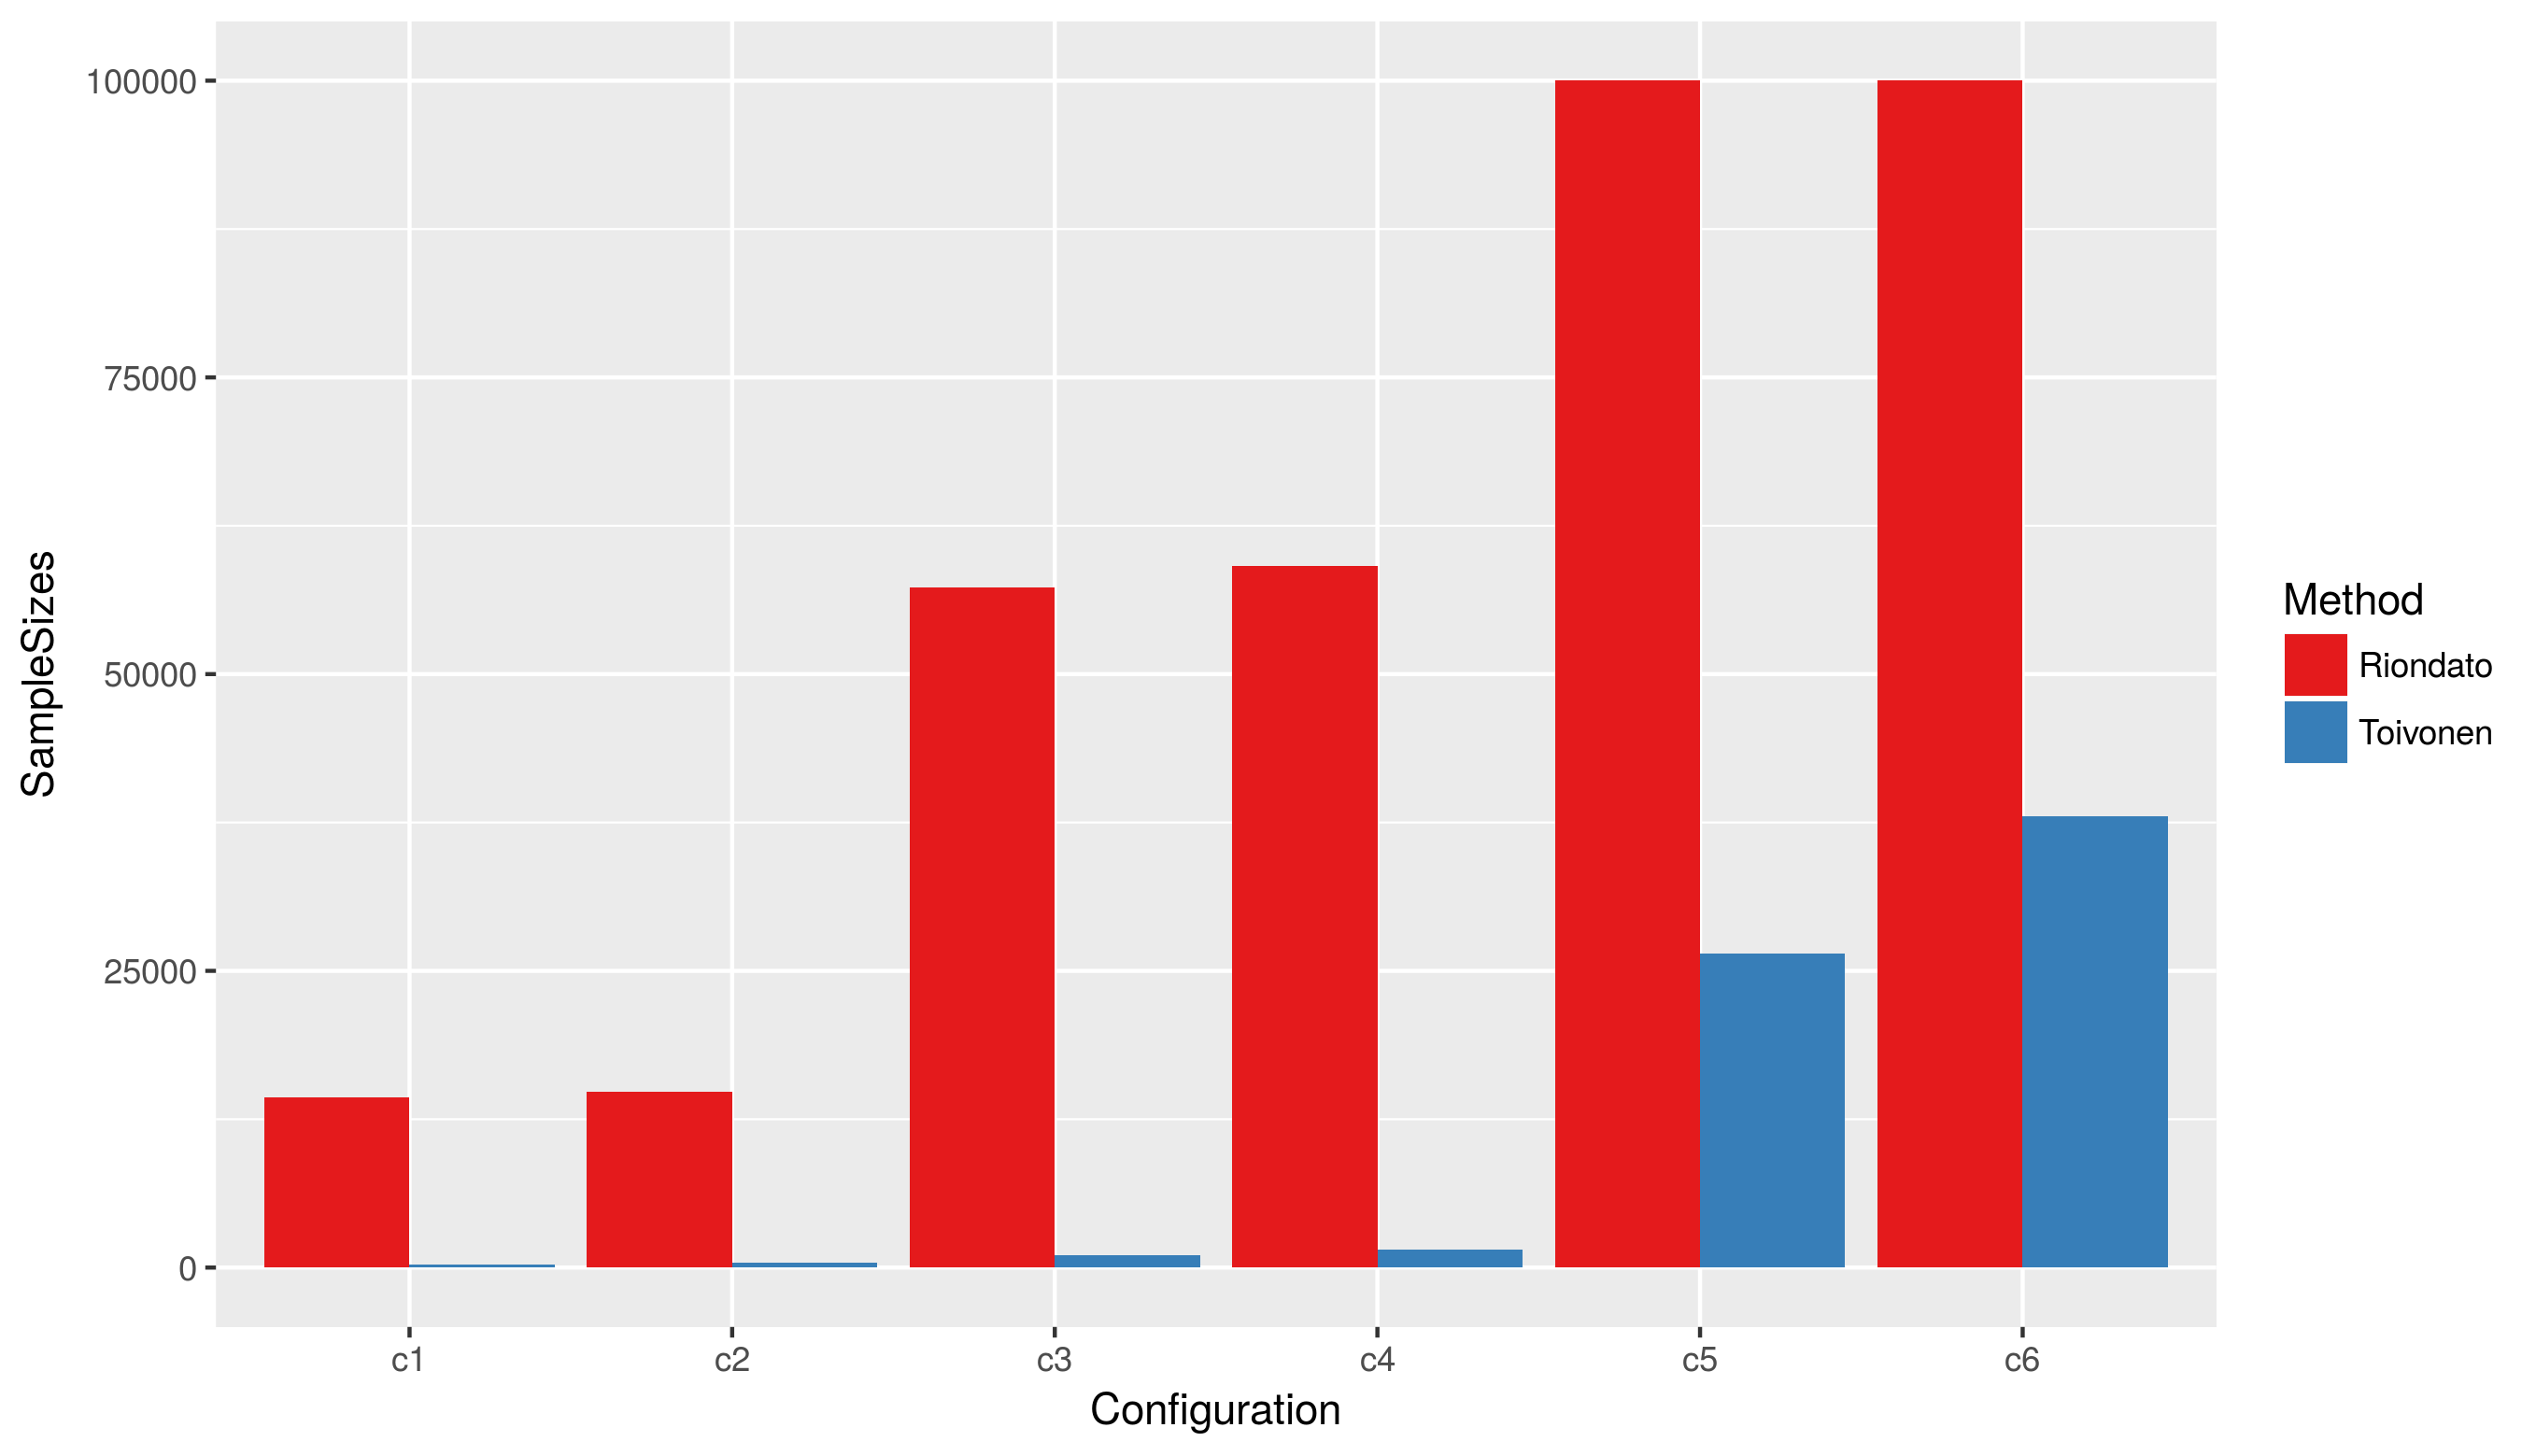
\includegraphics[width=\columnwidth]{T40I10D100K.dat/sampleSizes.png}
\end{figure}

It is immediately evident that Toivonen's approach requires much smaller samples. This is in contradiction with the claim in Riondato's paper that previous work (incl. Toivonen) suggests sample sizes that are linearly dependent on the total number of items $|\I|$. In fact, the Toivonen sample size is not dependent on $\I$, as witnessed by the bound:
\[ n \geq \frac{1}{2\epsilon^2}ln\frac{2}{\delta} 
\]

Another important remark is that, when the parameters get rather demanding (i.e. $c_5,\ c_6$), Riondato's approach eventually requires a sample the size of the whole dataset.

\subsubsection{Precision-Recall}
Before we display the precision and recall metrics, it is clarifying to see the percentage rates of the involved underlying quantities (i.e. true-positives, false-positives and false-negatives). We render them in pie charts, representing true-positives with \textcolor{green}{green}, false-positives with \textcolor{red}{red} and false-negatives with \textcolor{blue}{blue}. Configurations are ordered top-to-bottom, left-to-right.
\begin{figure}[h!]
\centering
\caption*{Toivonen}
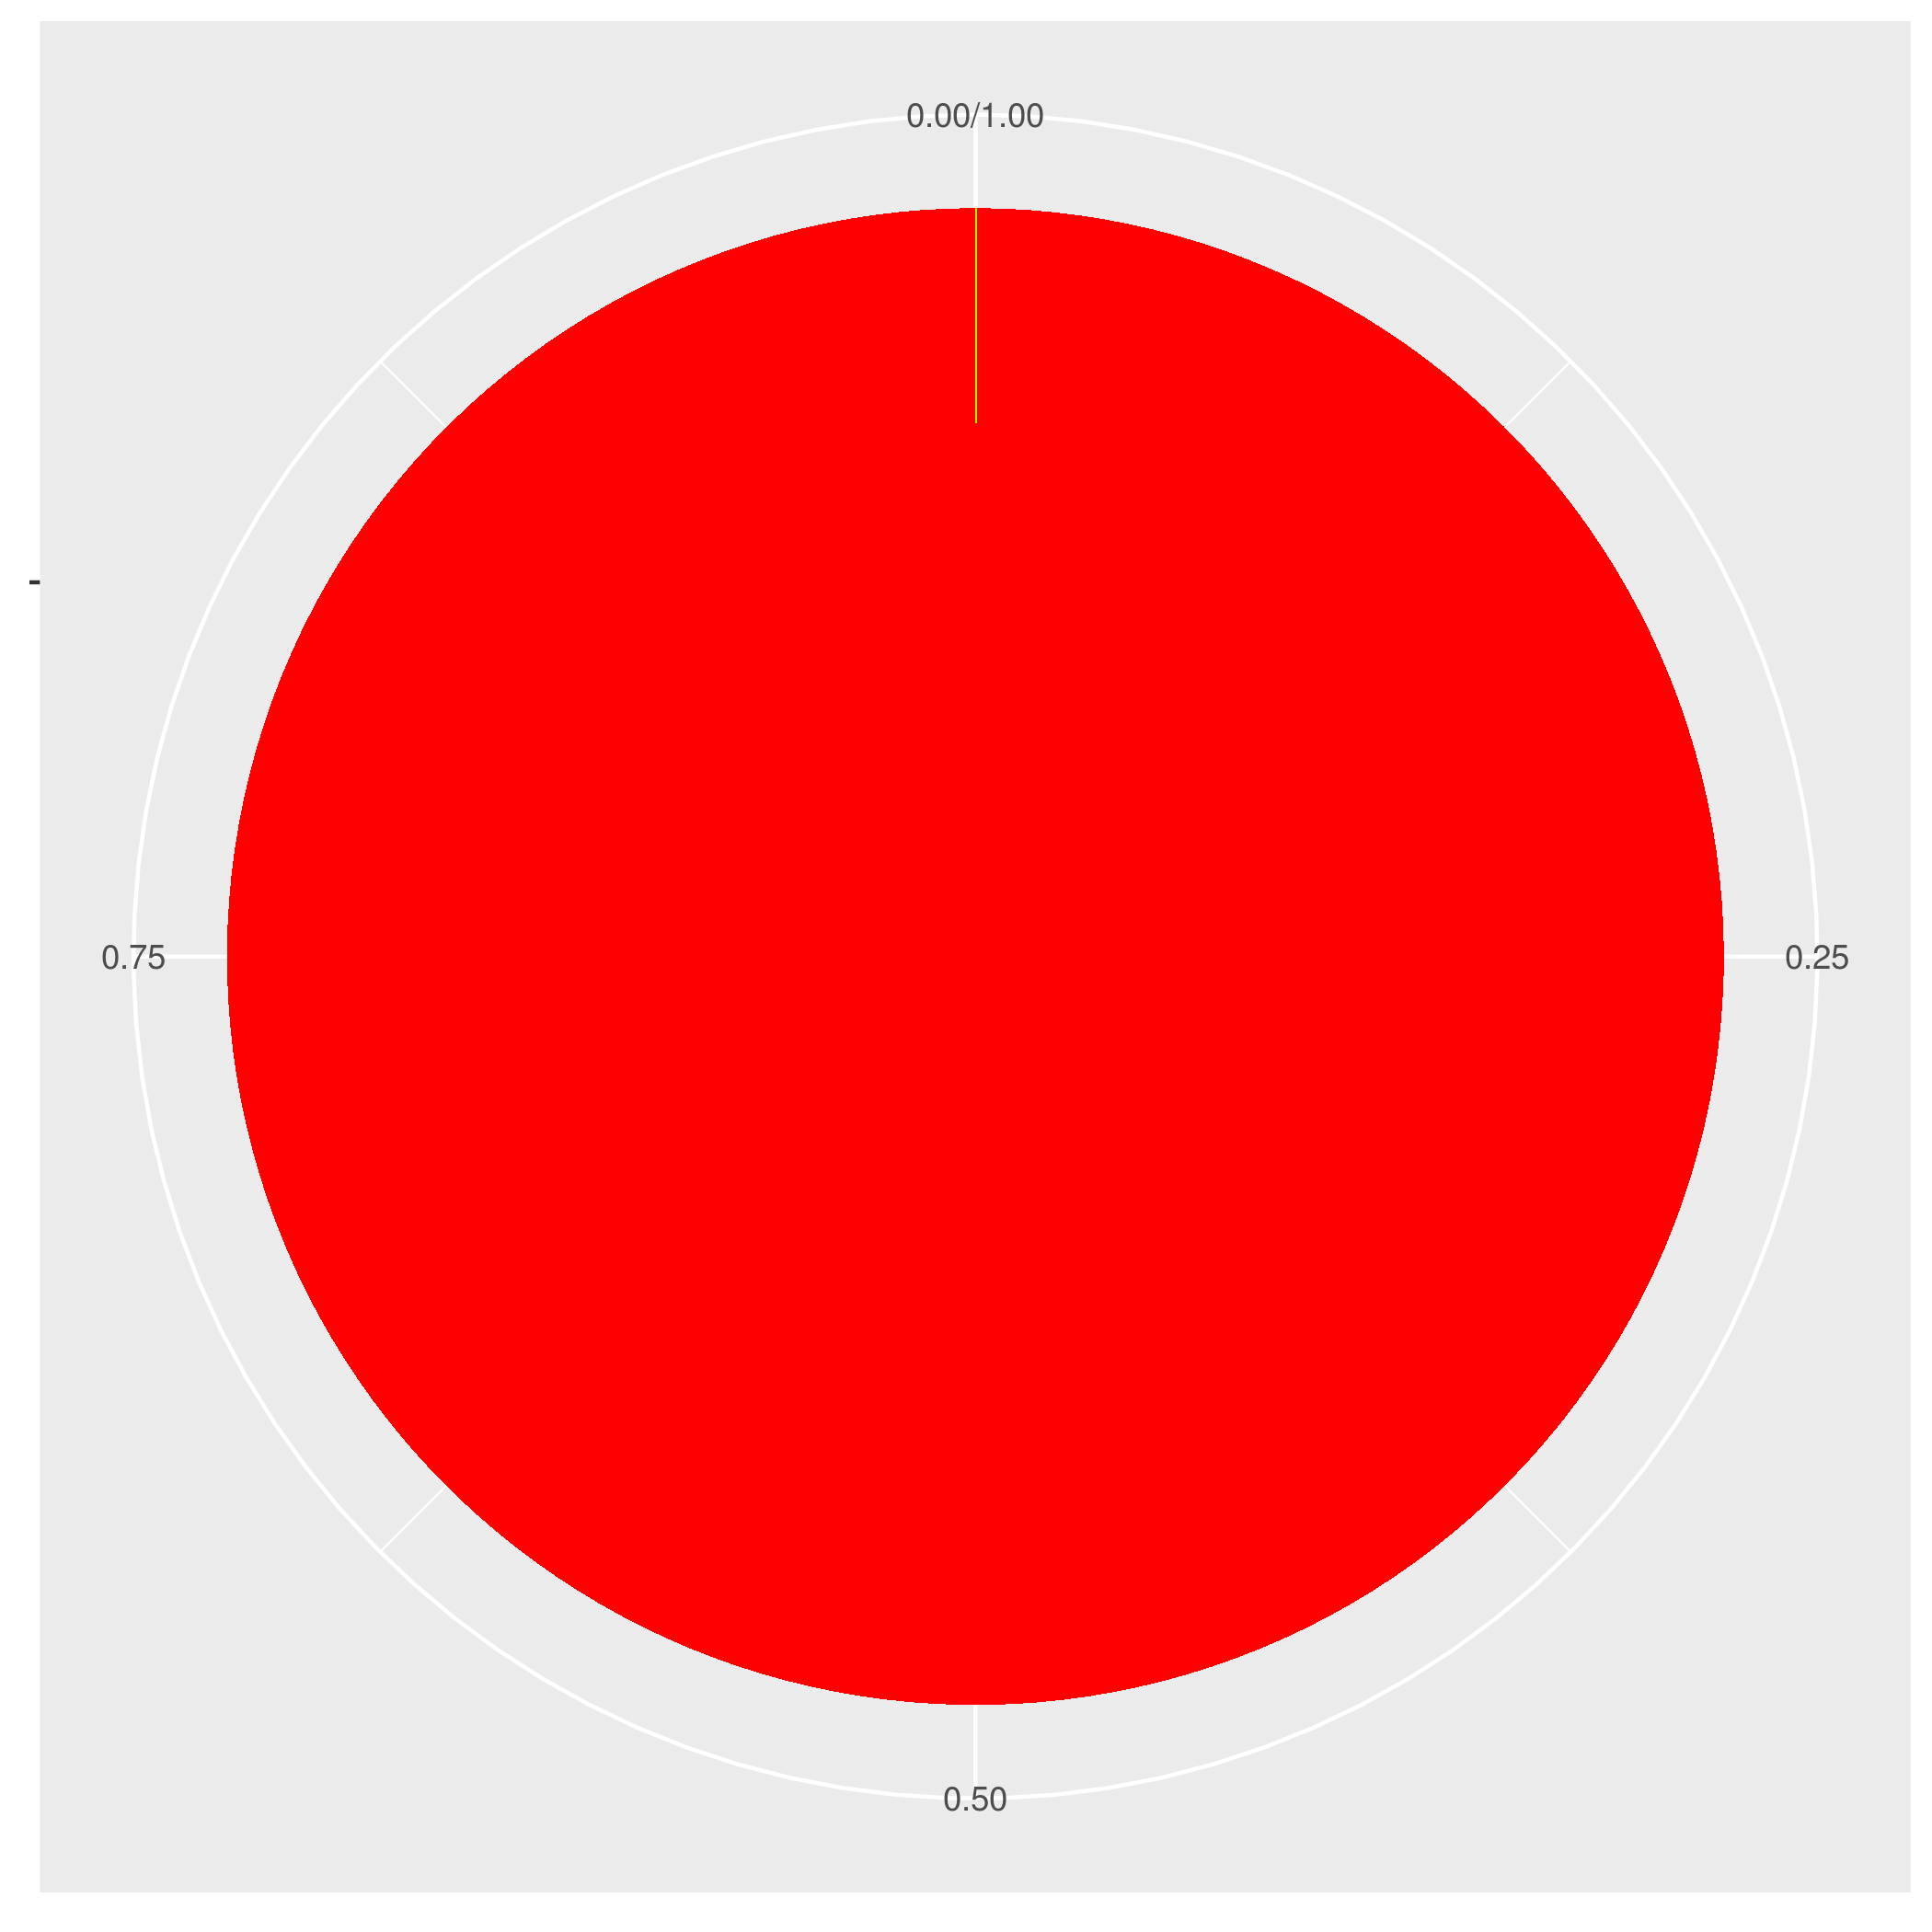
\includegraphics[width=.25\columnwidth]{T40I10D100K.dat/toivonen-c1.png}
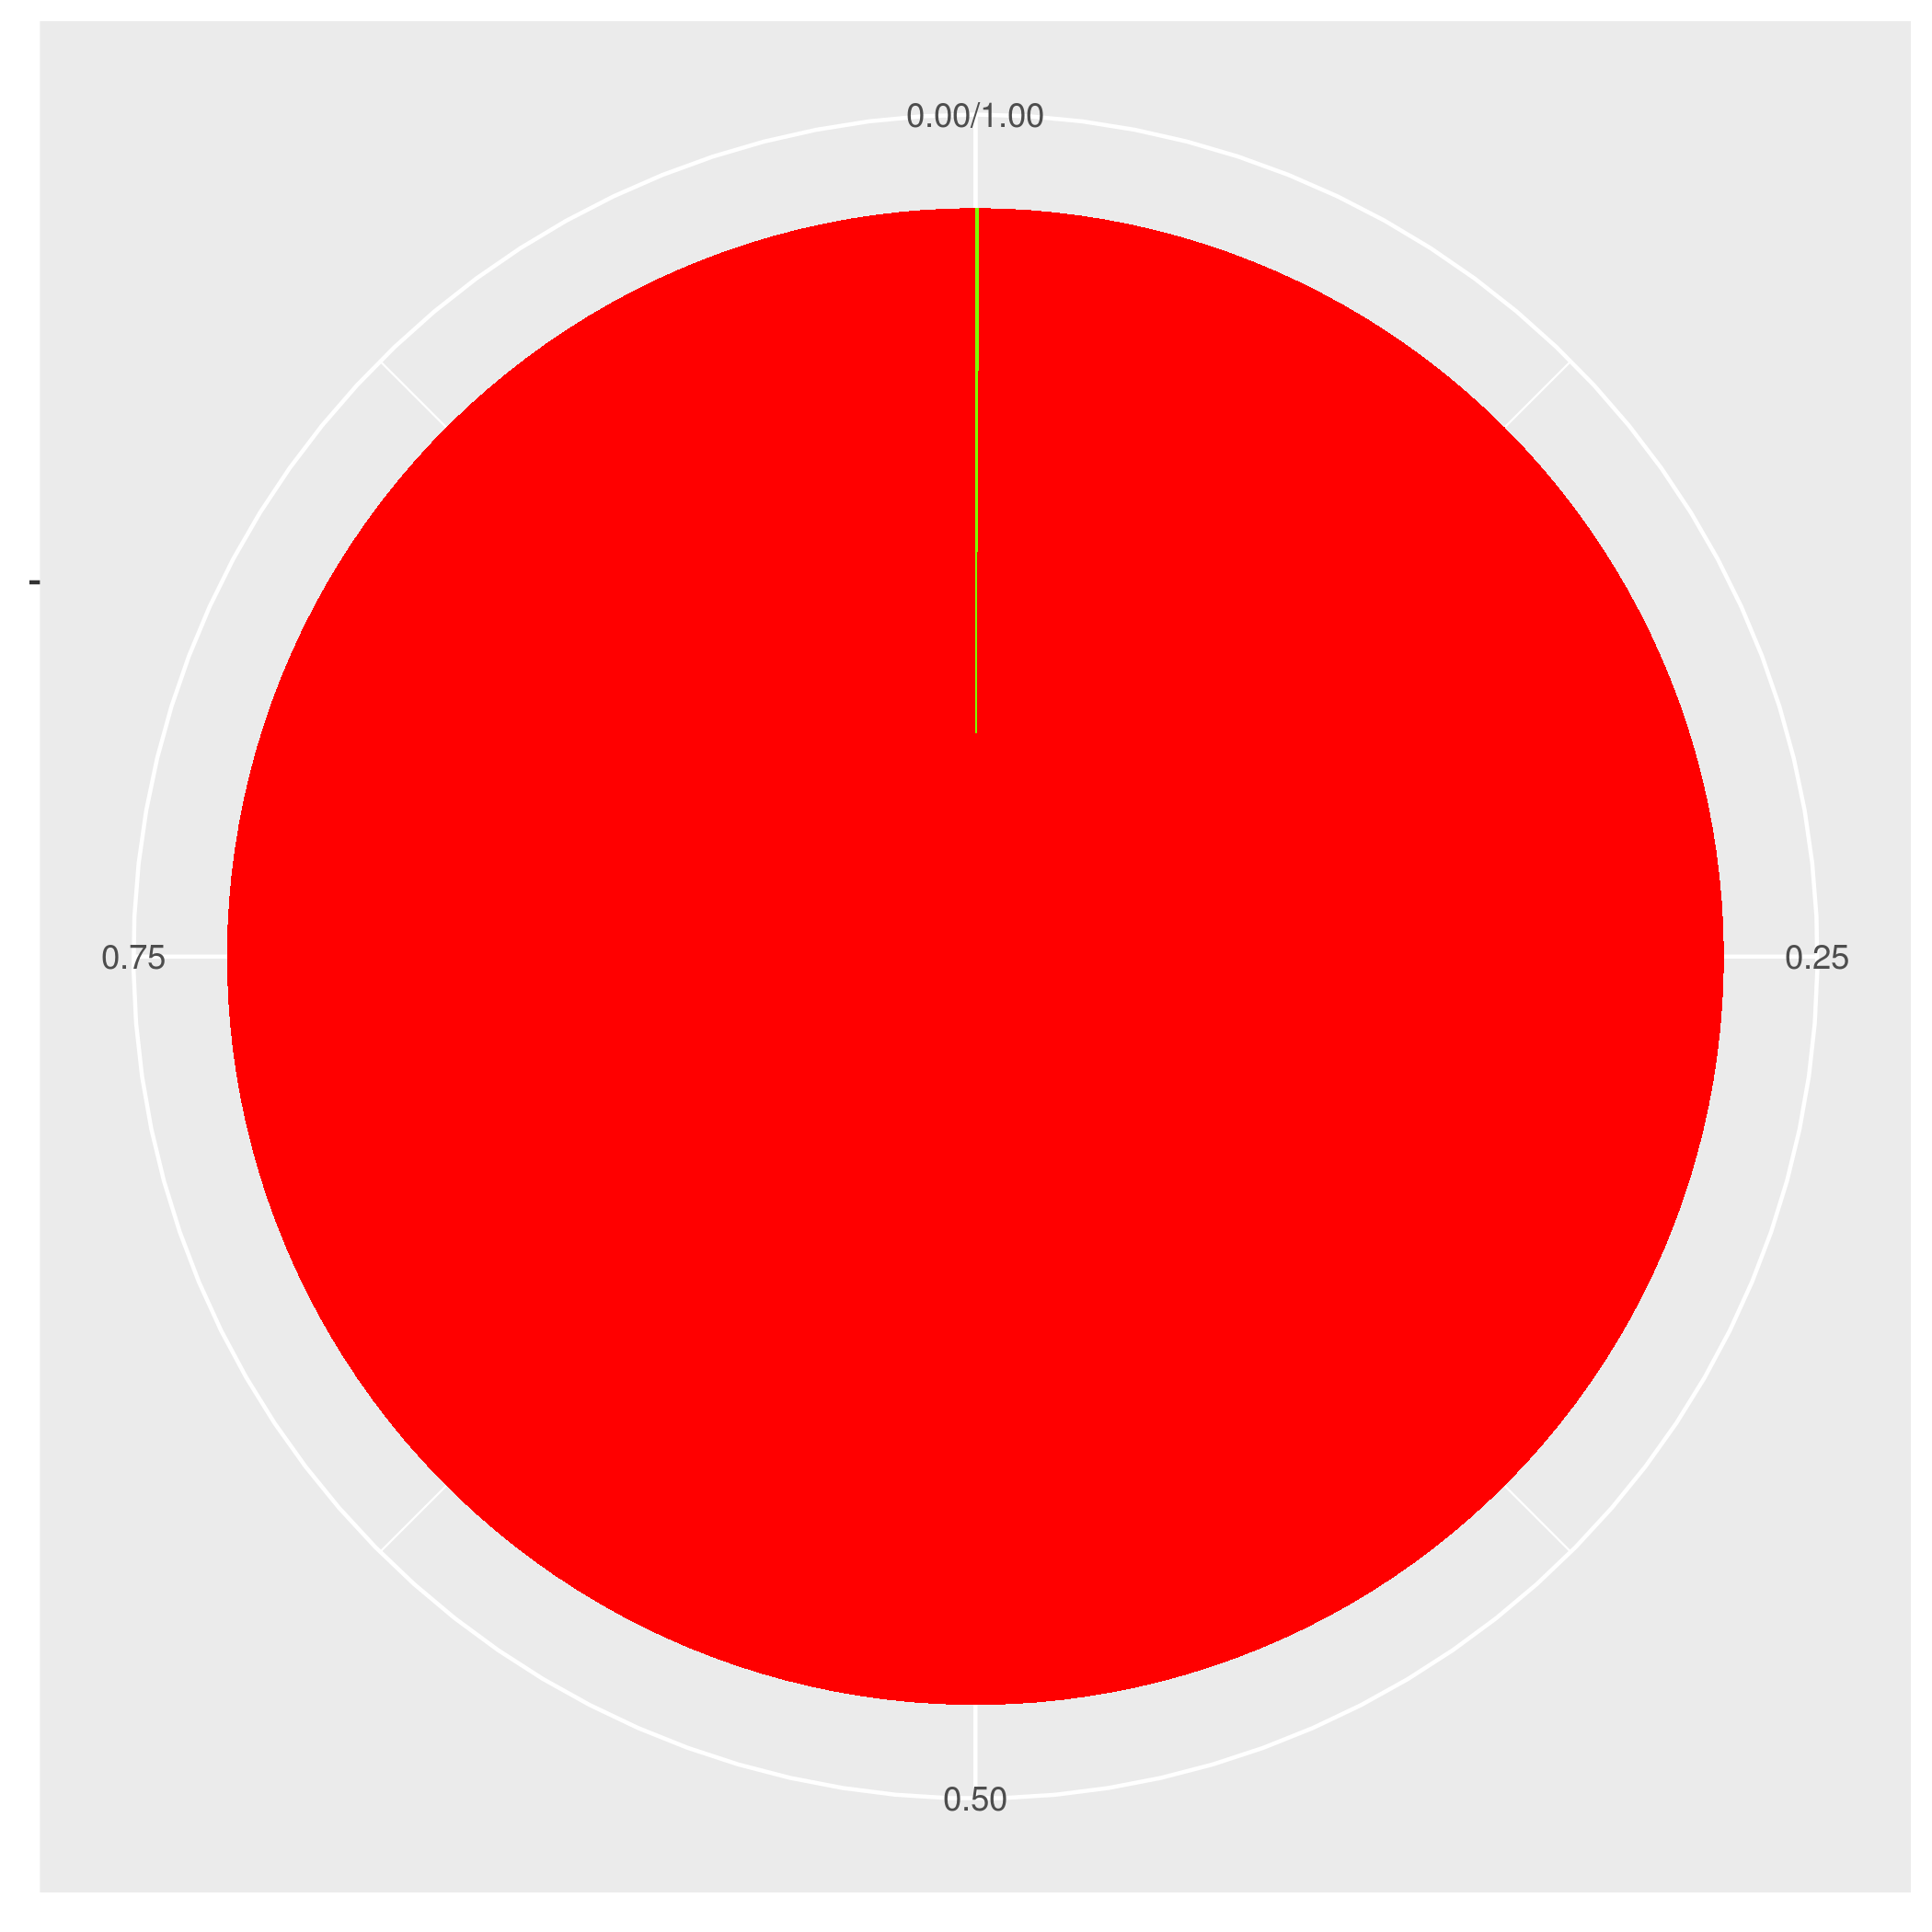
\includegraphics[width=.25\columnwidth]{T40I10D100K.dat/toivonen-c2.png}
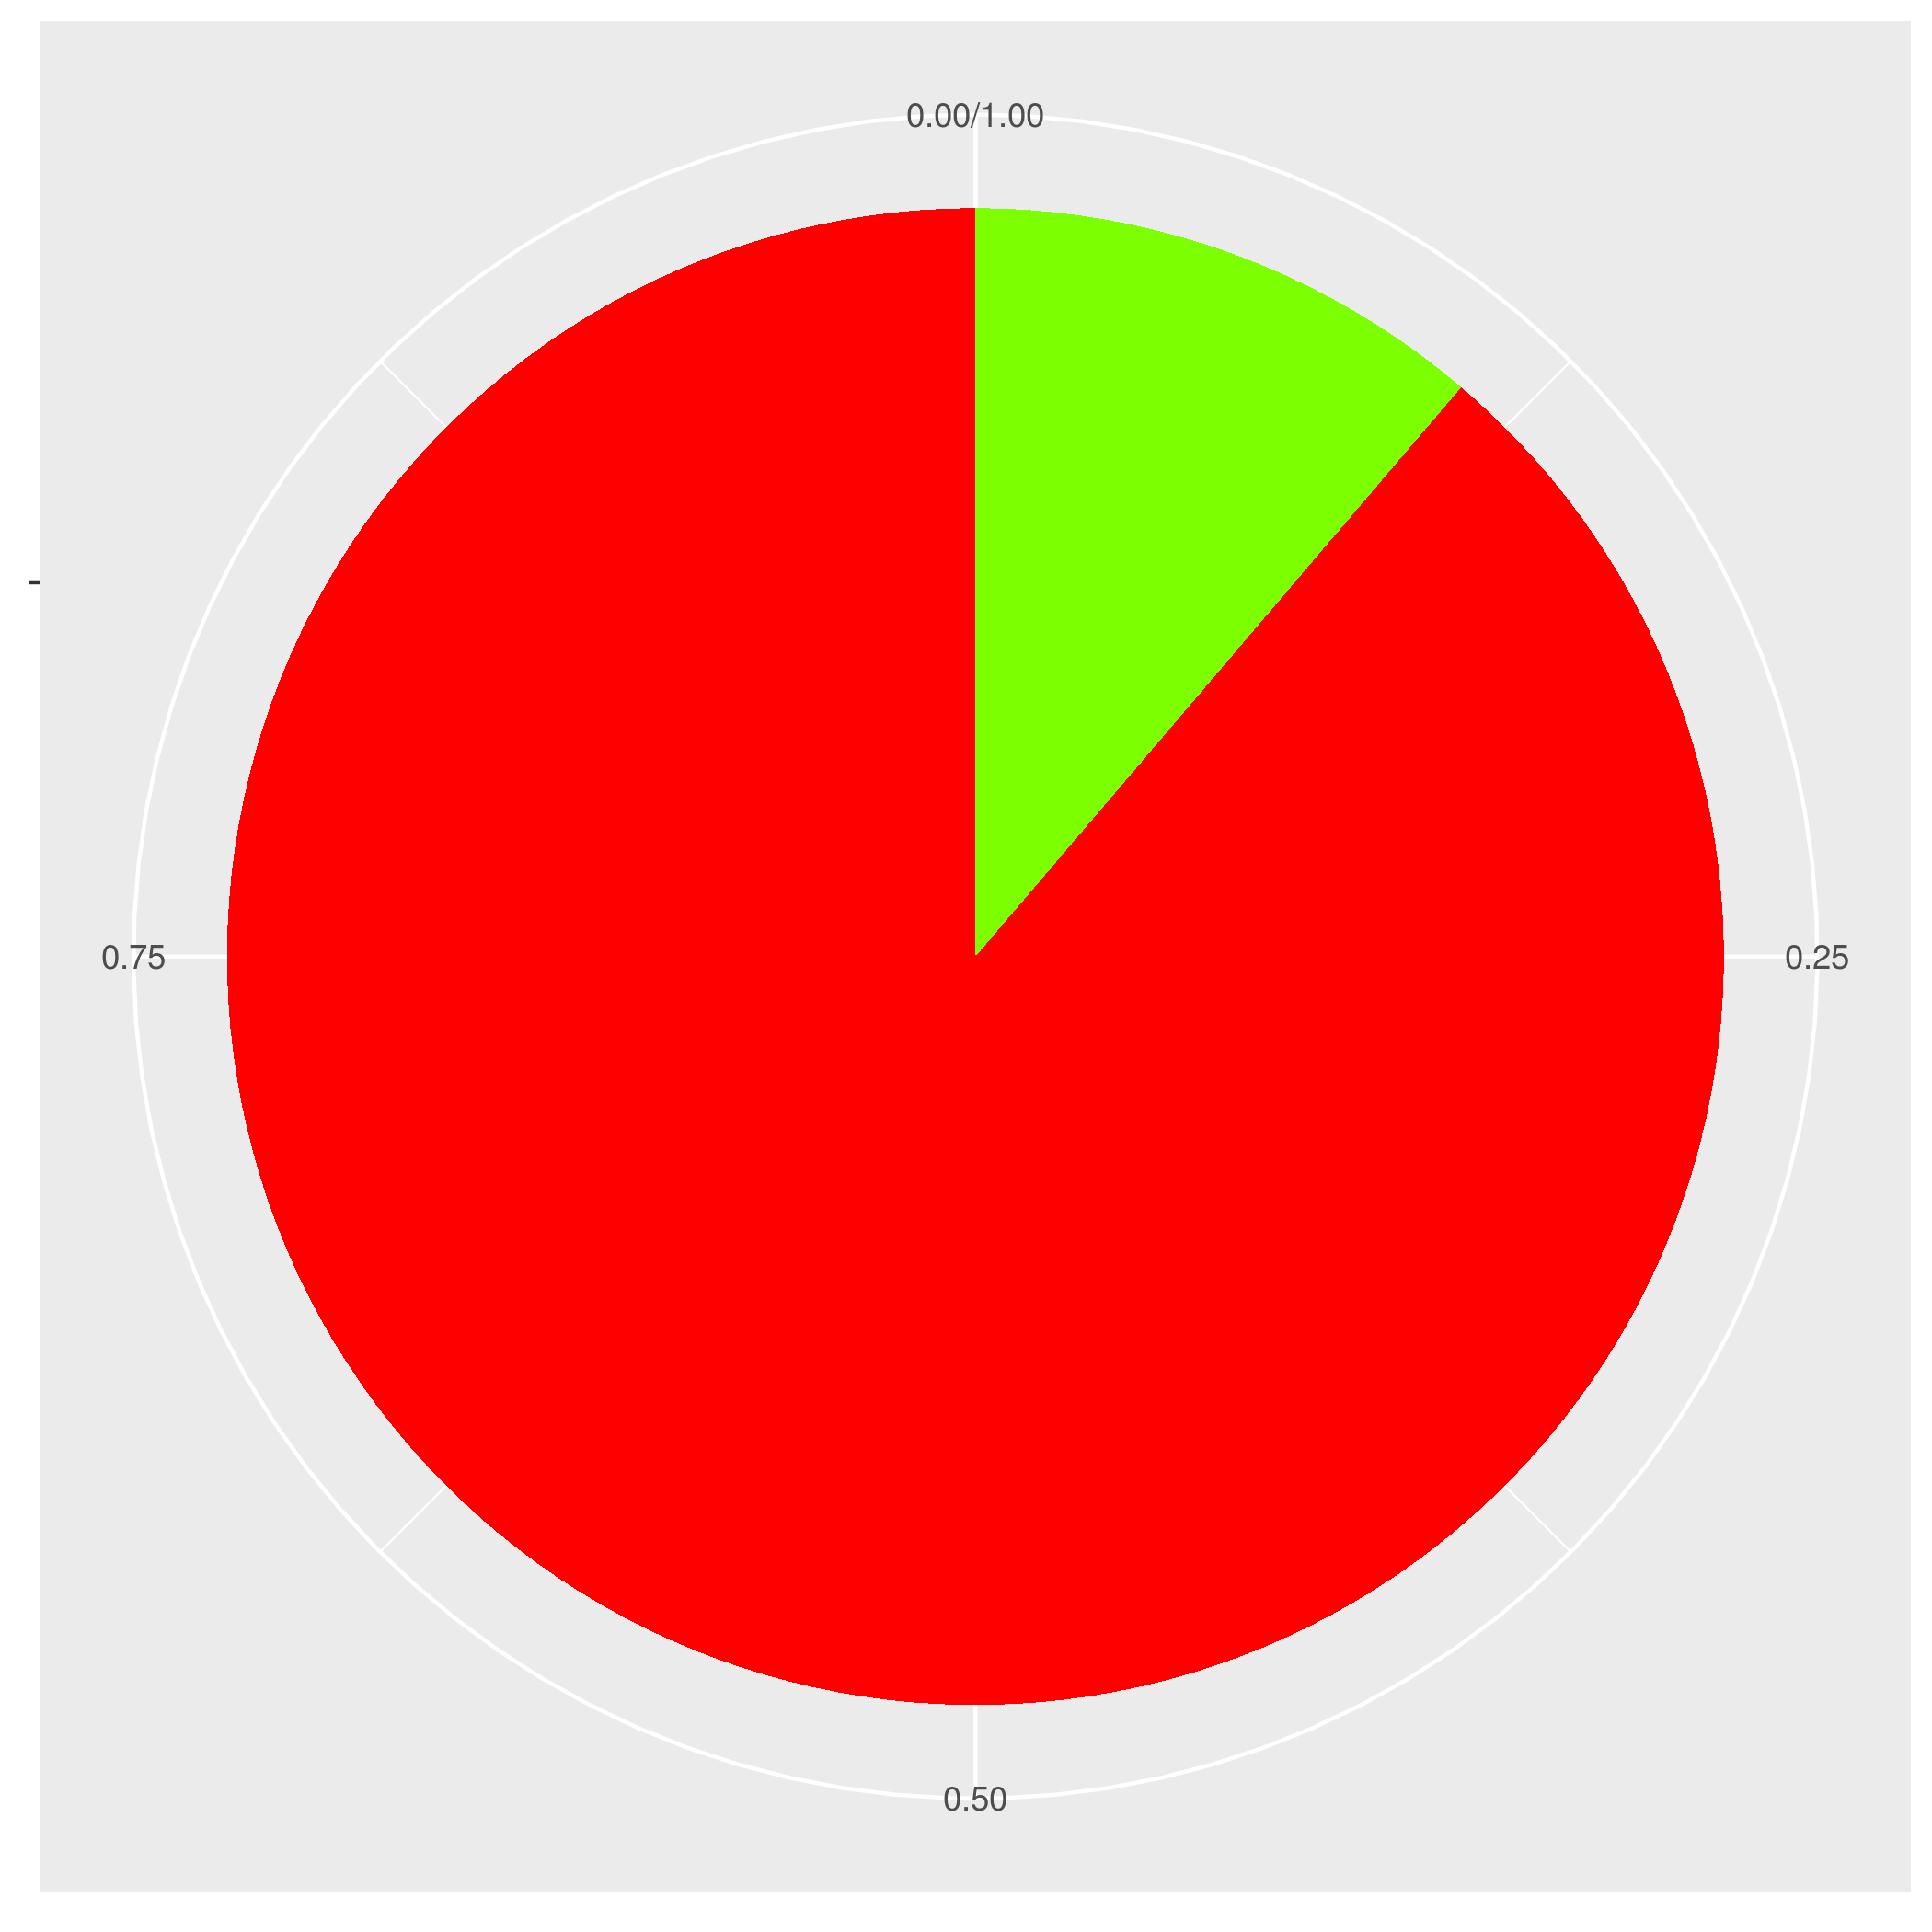
\includegraphics[width=.25\columnwidth]{T40I10D100K.dat/toivonen-c3.png}\\
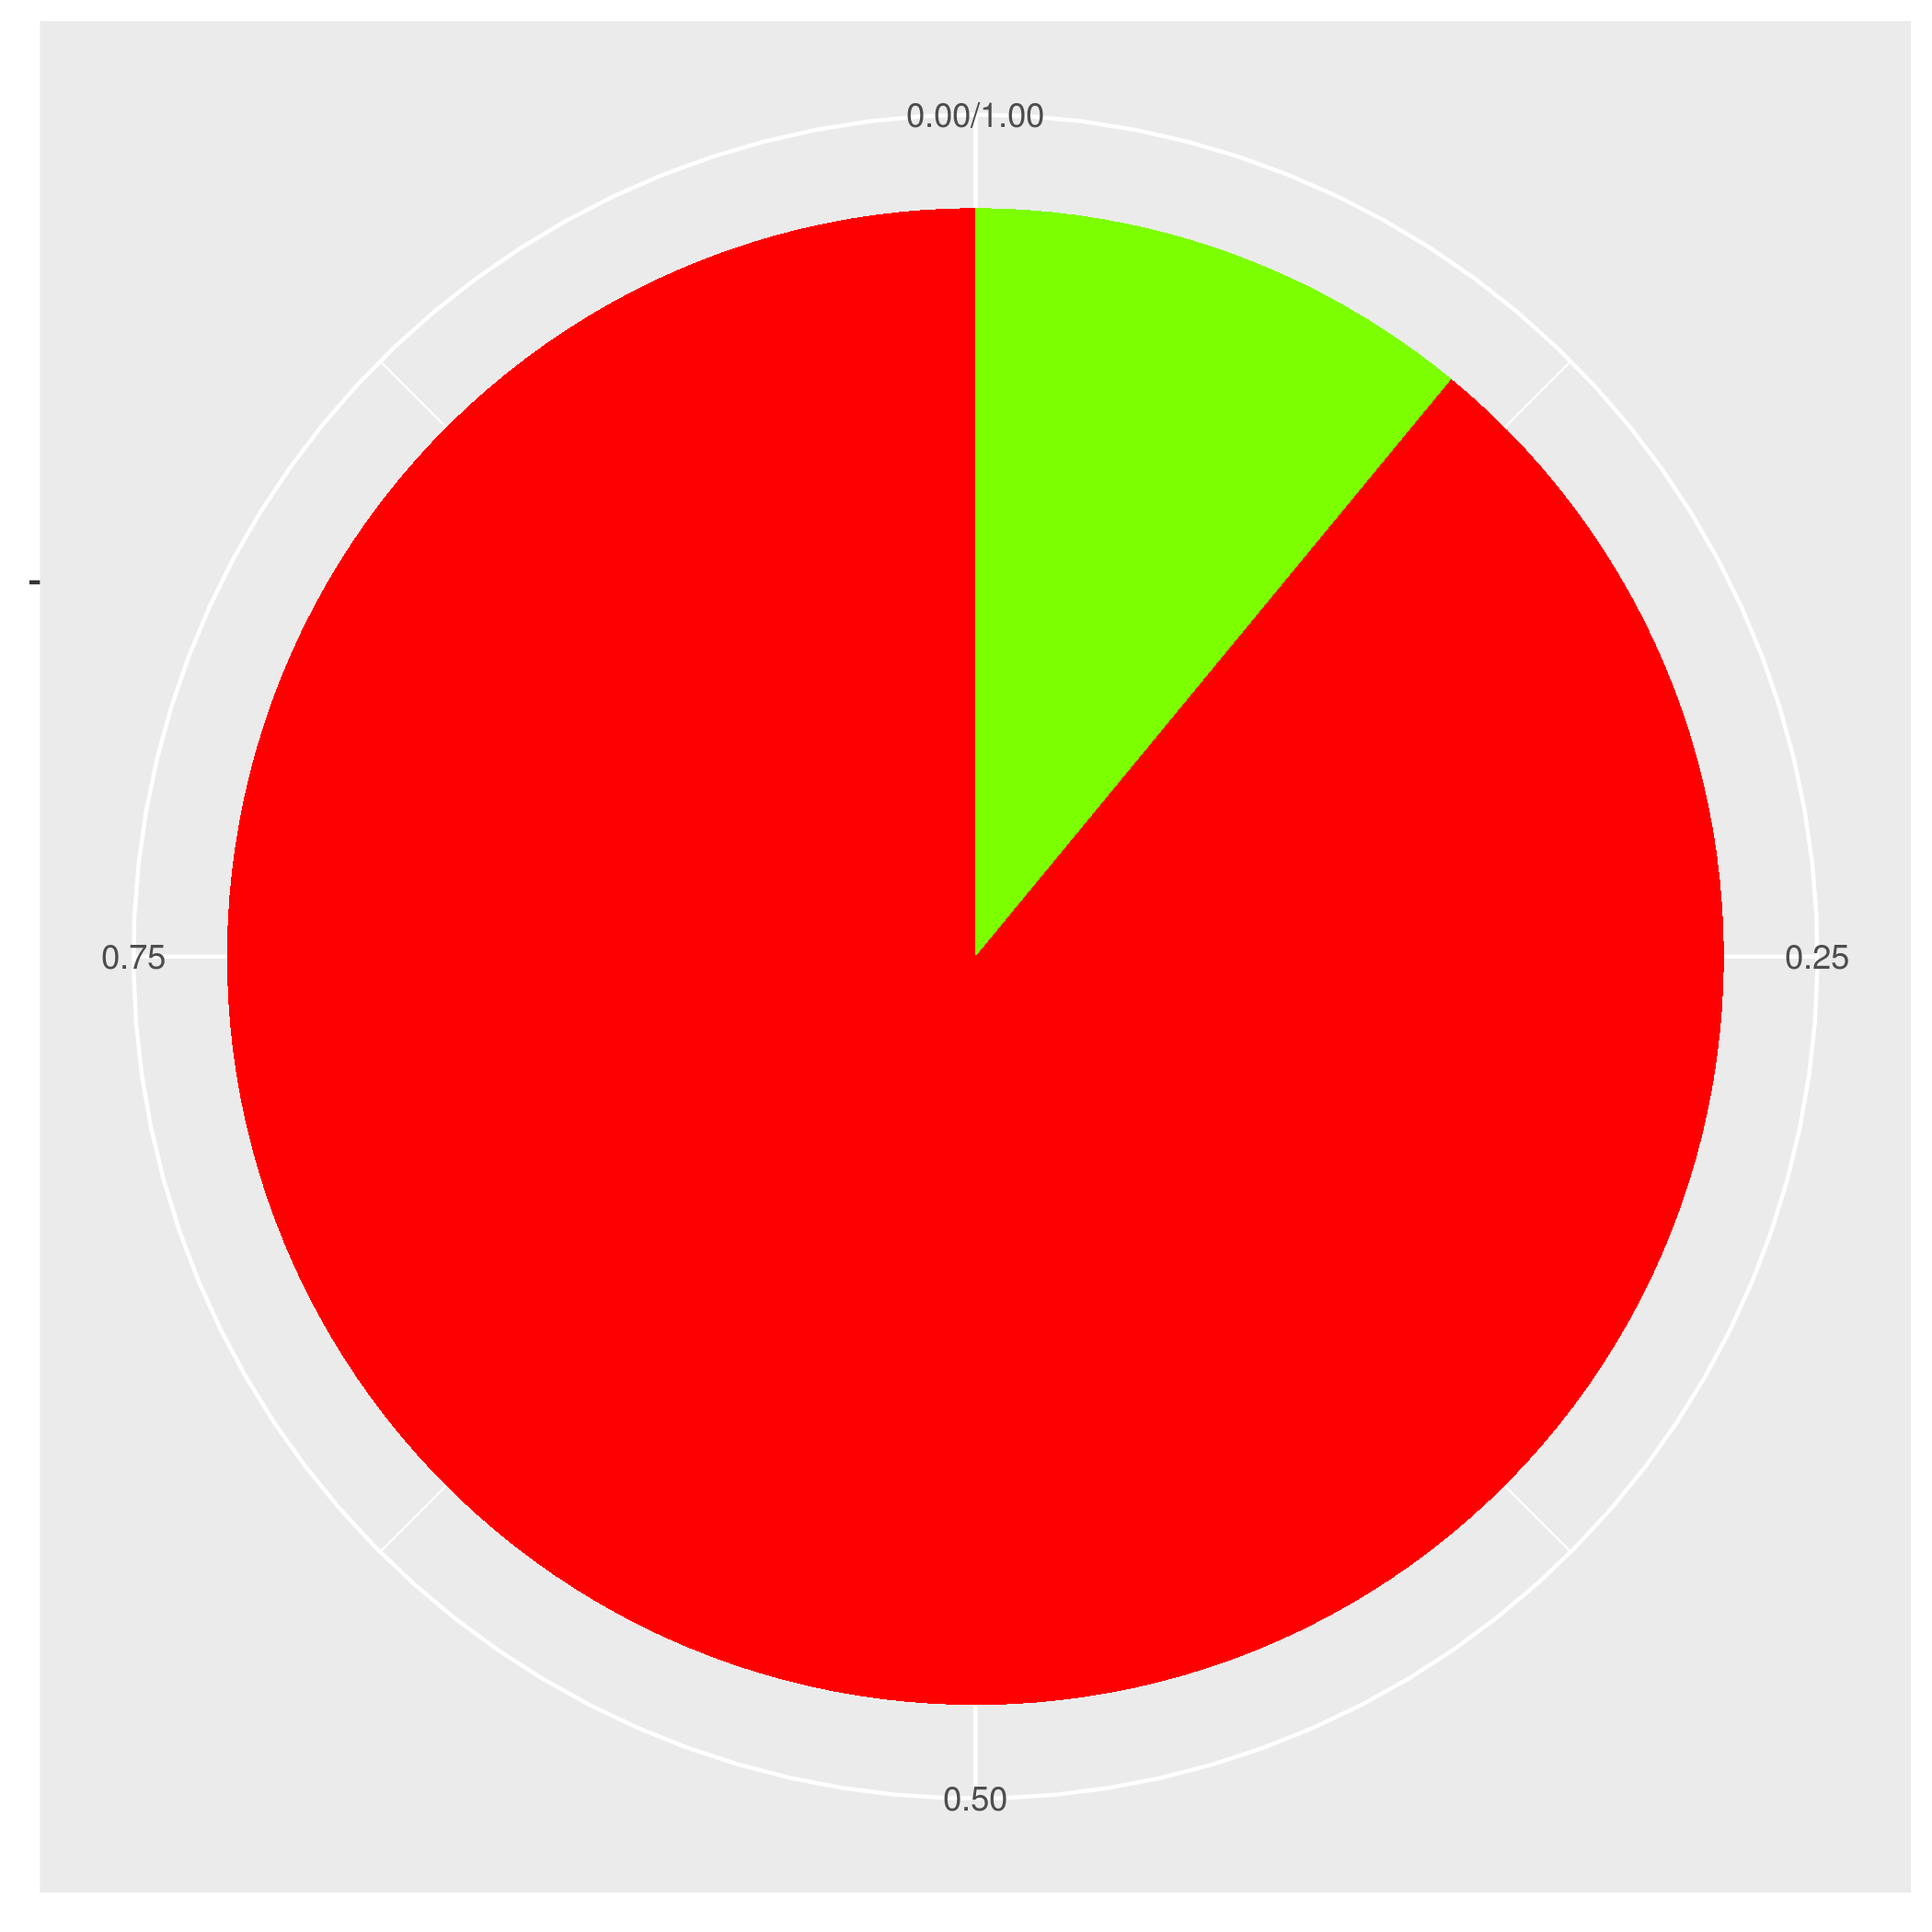
\includegraphics[width=.25\columnwidth]{T40I10D100K.dat/toivonen-c4.png}
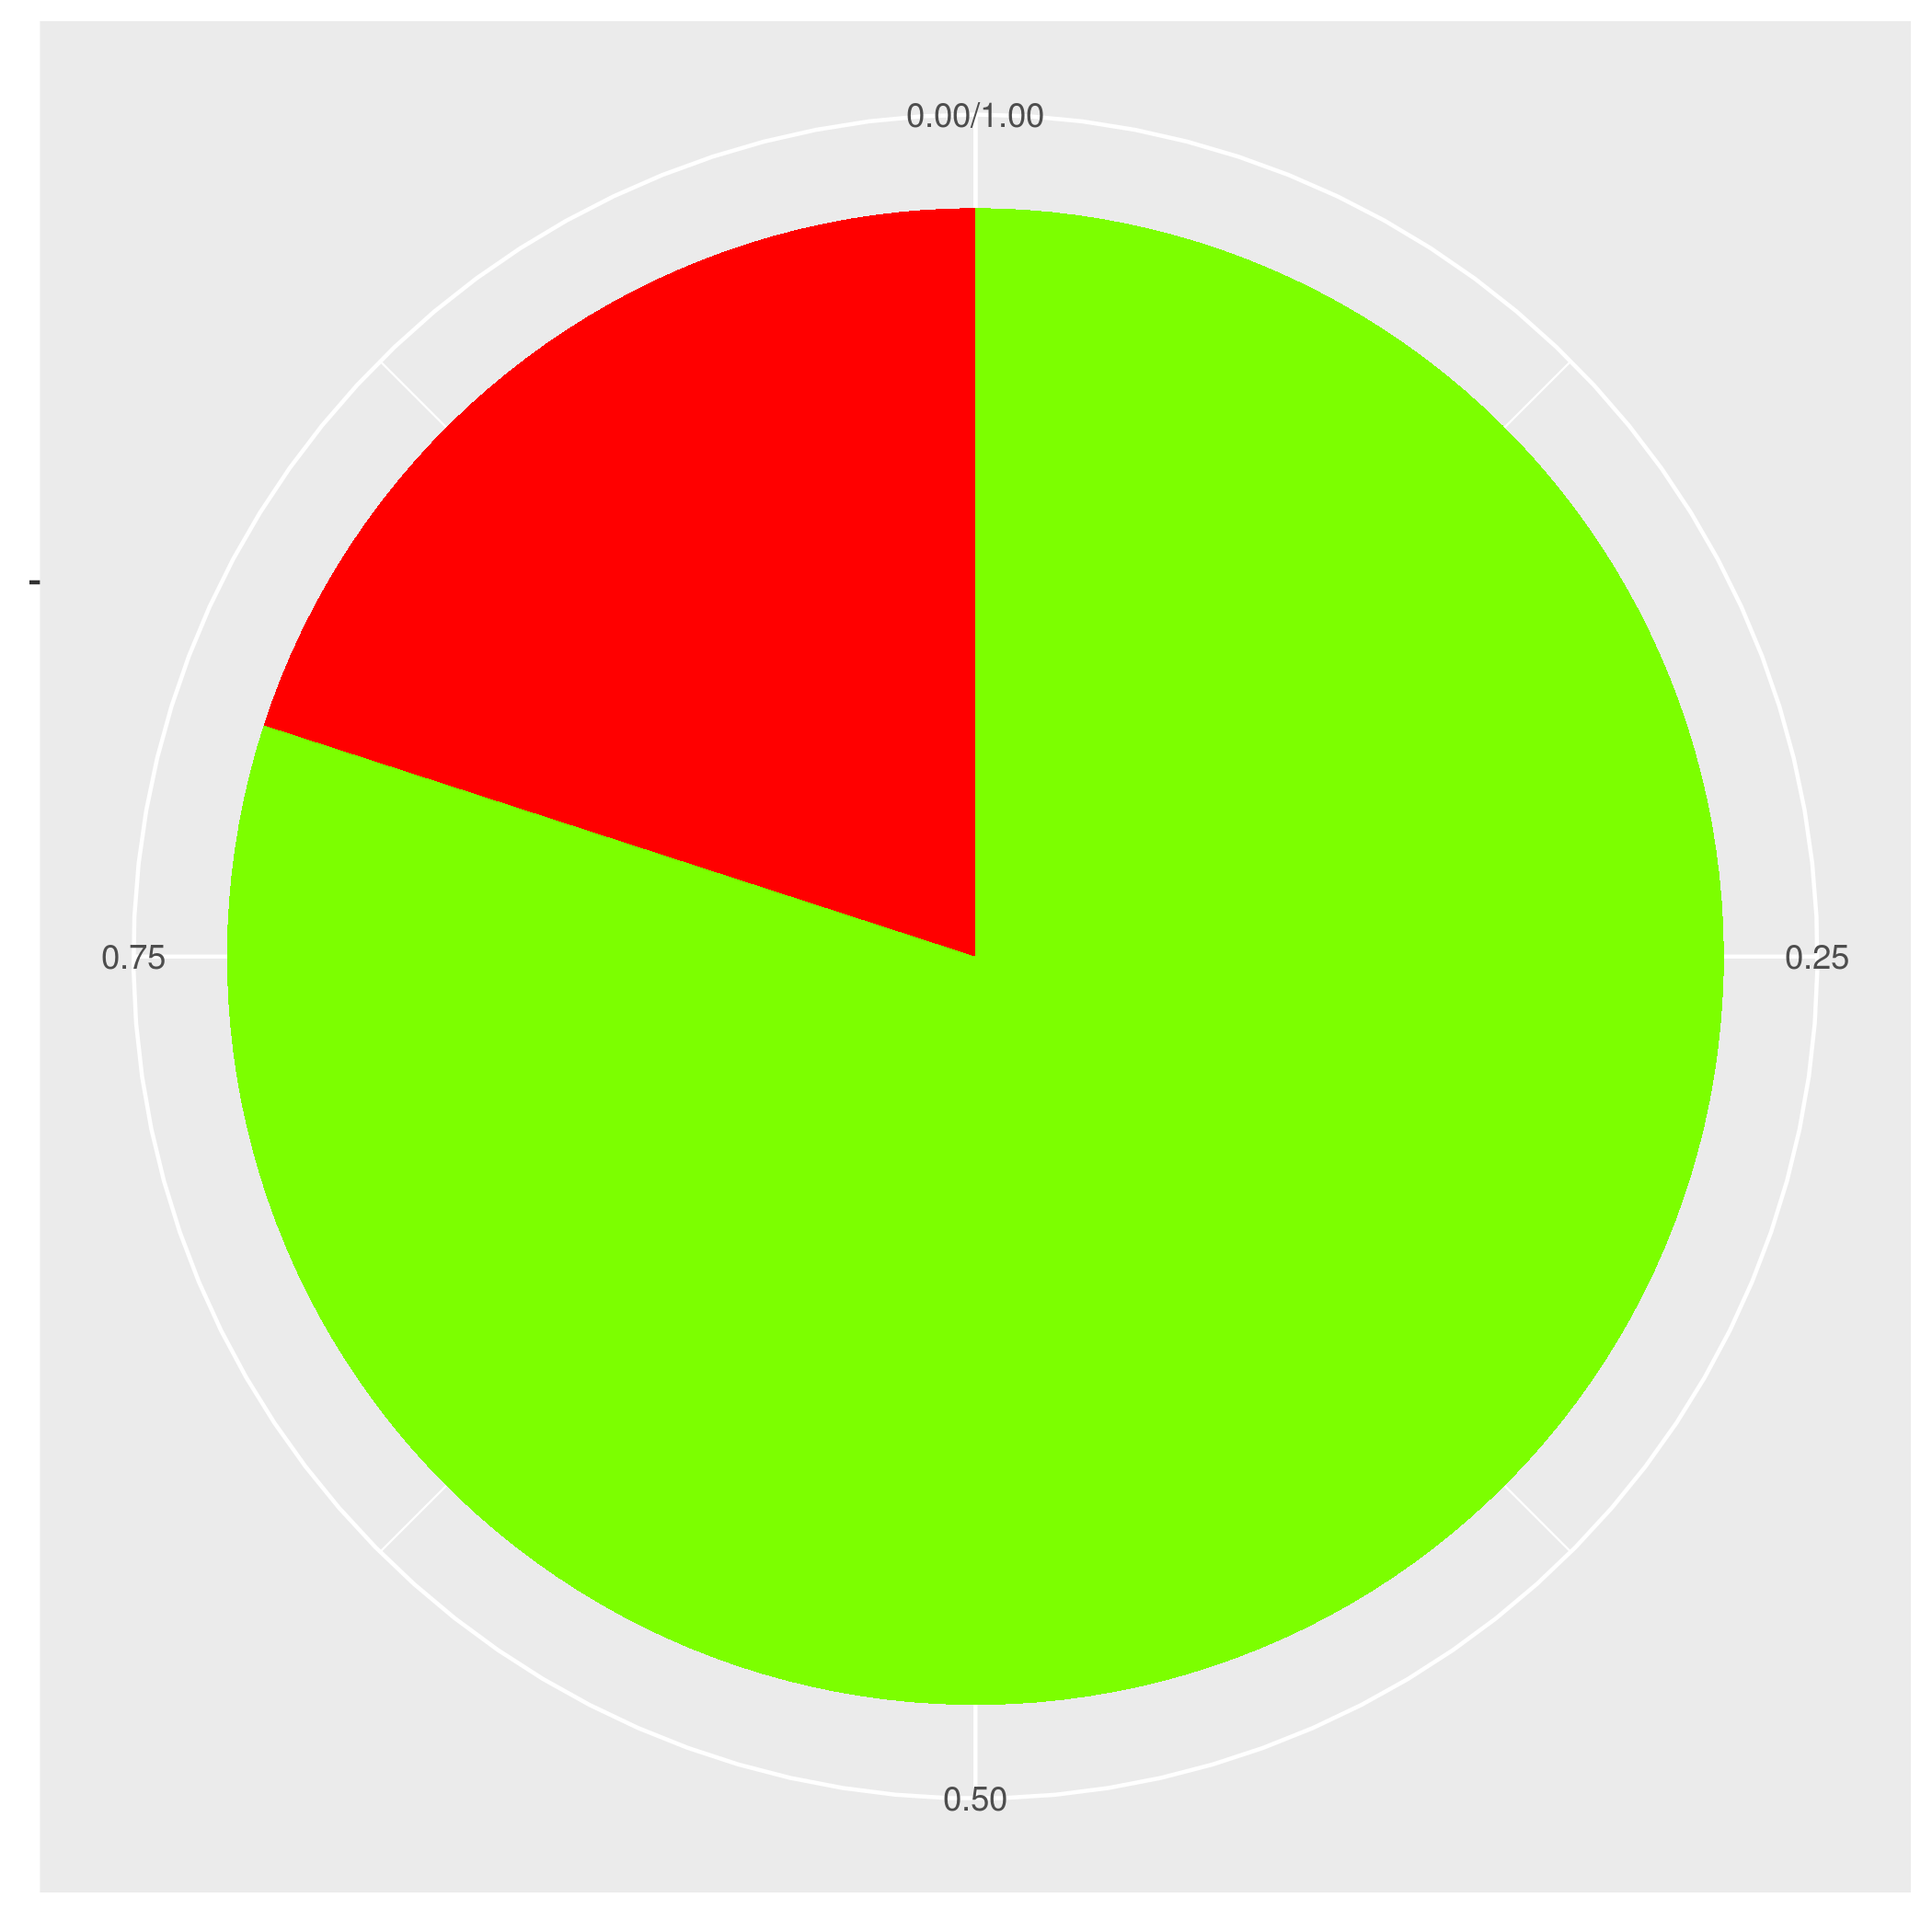
\includegraphics[width=.25\columnwidth]{T40I10D100K.dat/toivonen-c5.png}
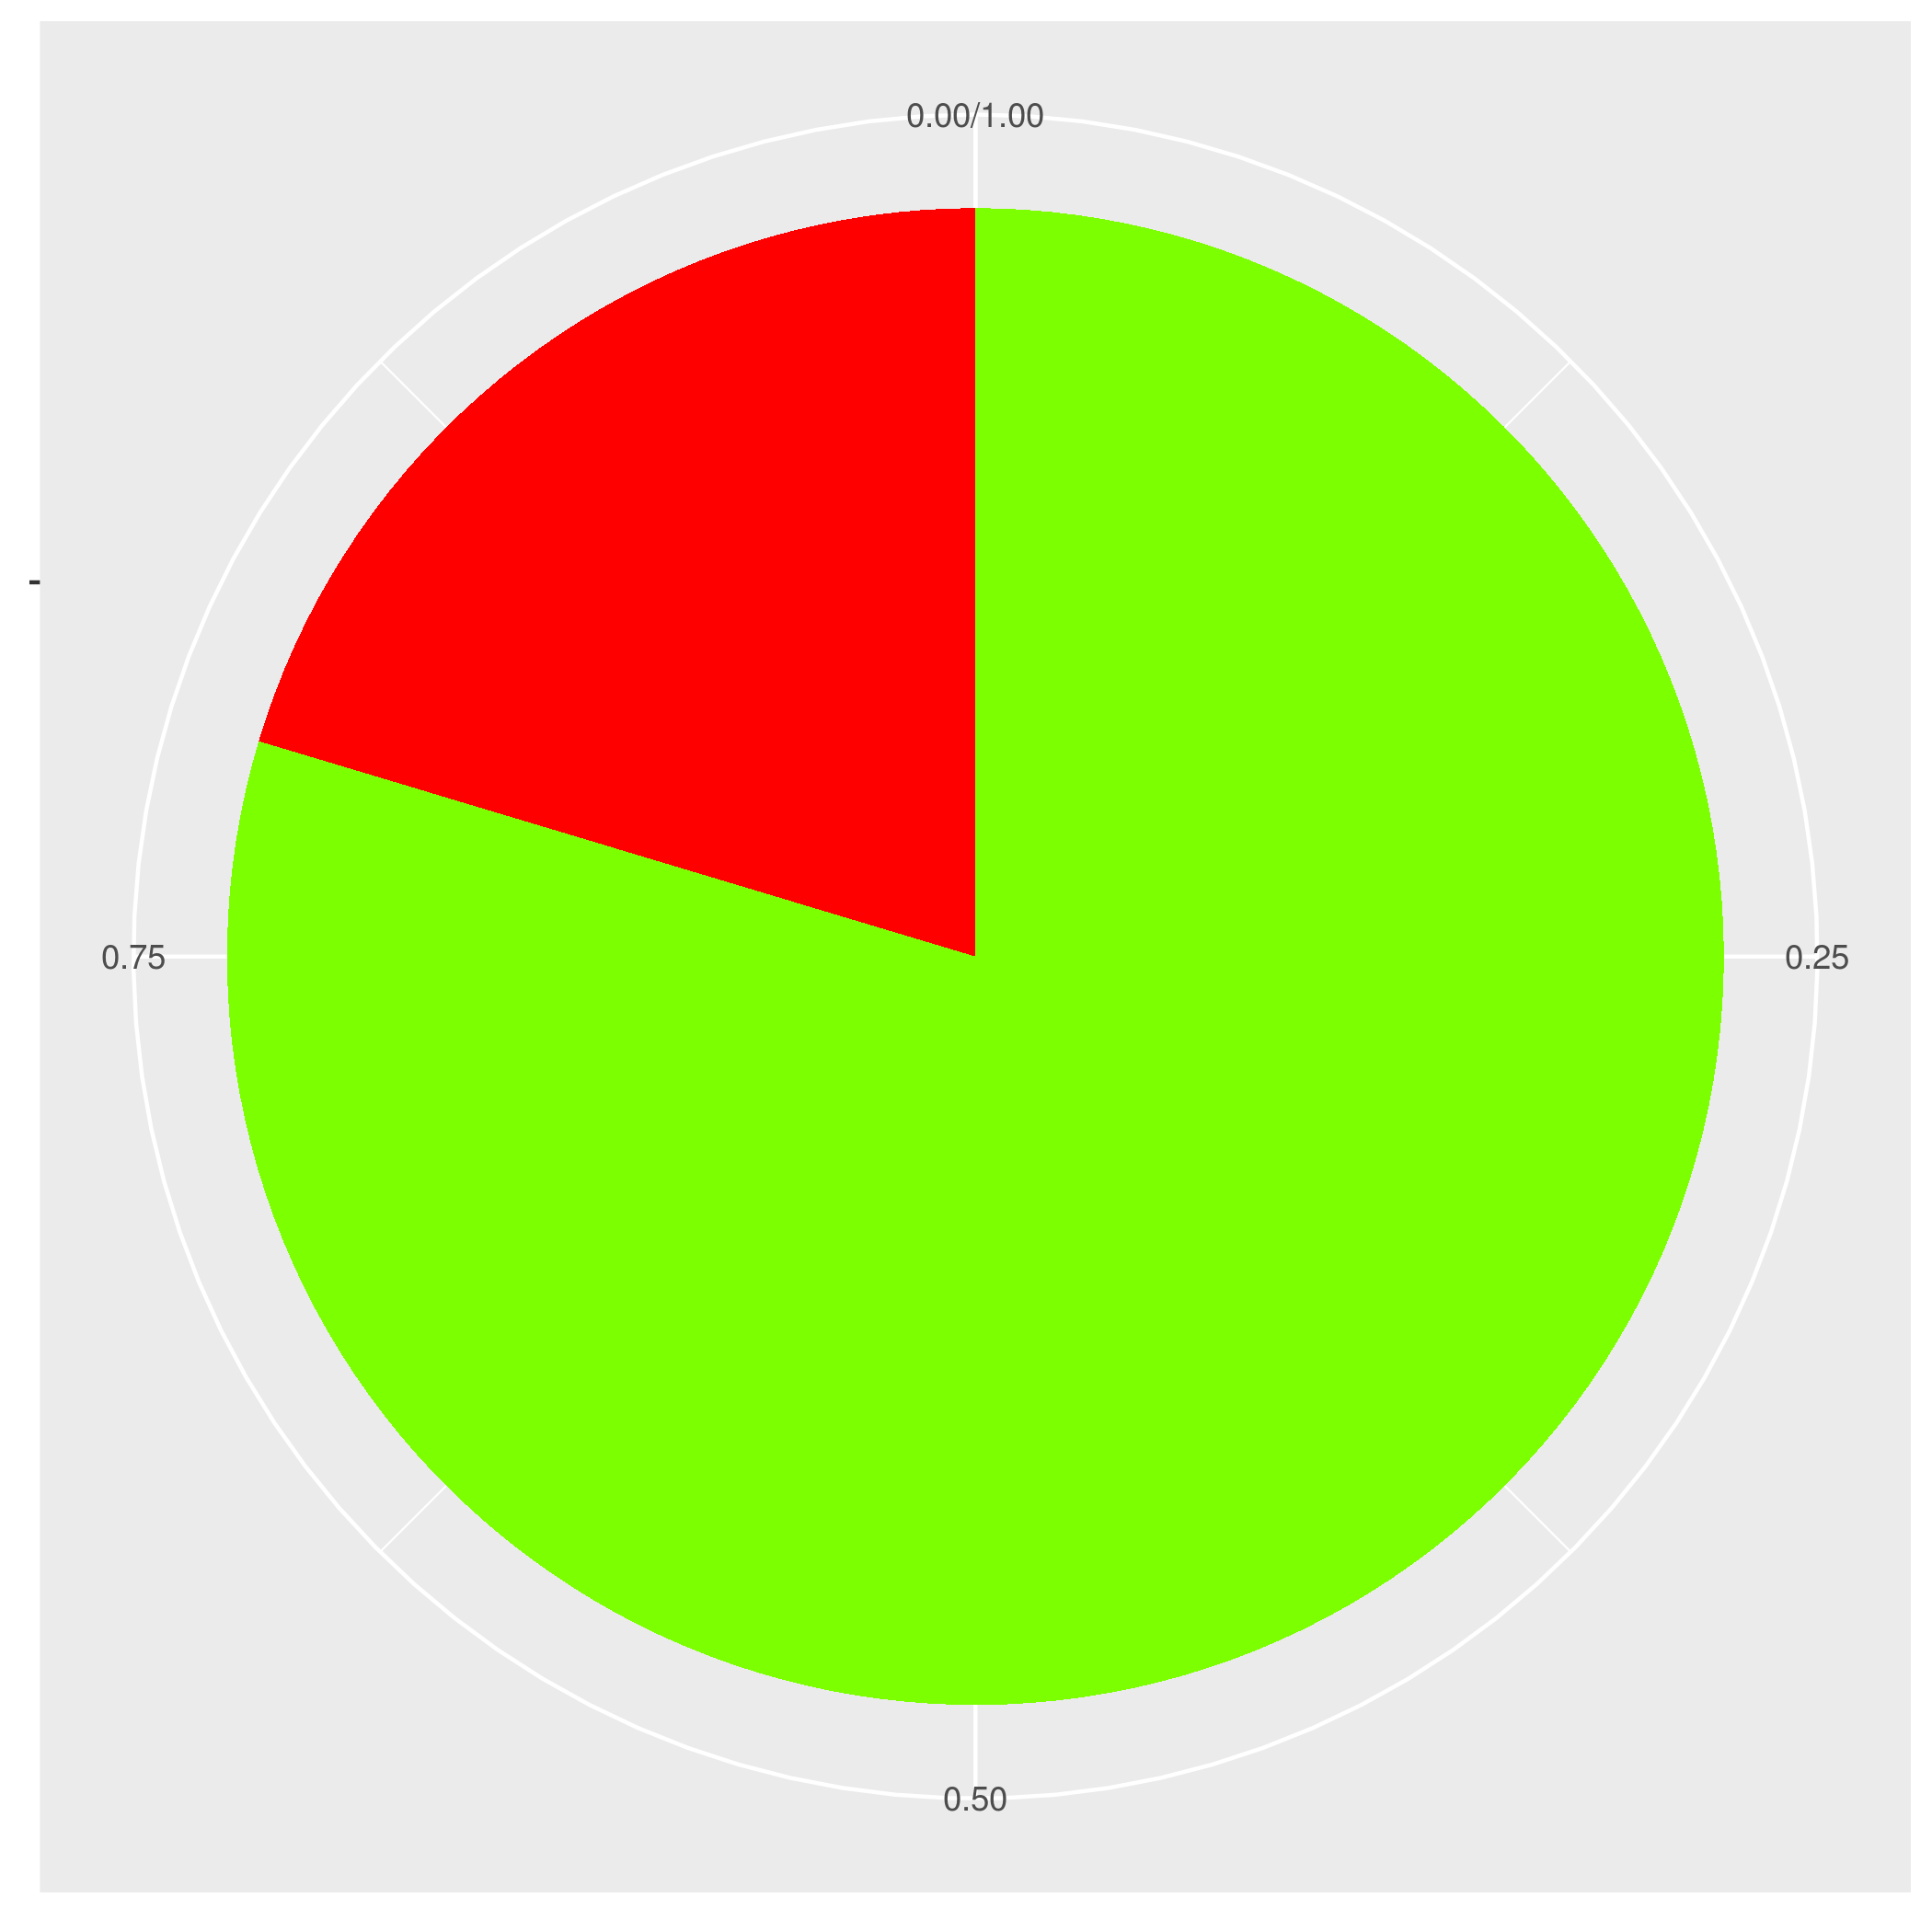
\includegraphics[width=.25\columnwidth]{T40I10D100K.dat/toivonen-c6.png}
\end{figure}
\vspace{-.45cm}
\begin{figure}[h!]
\centering
\caption*{Riondato}
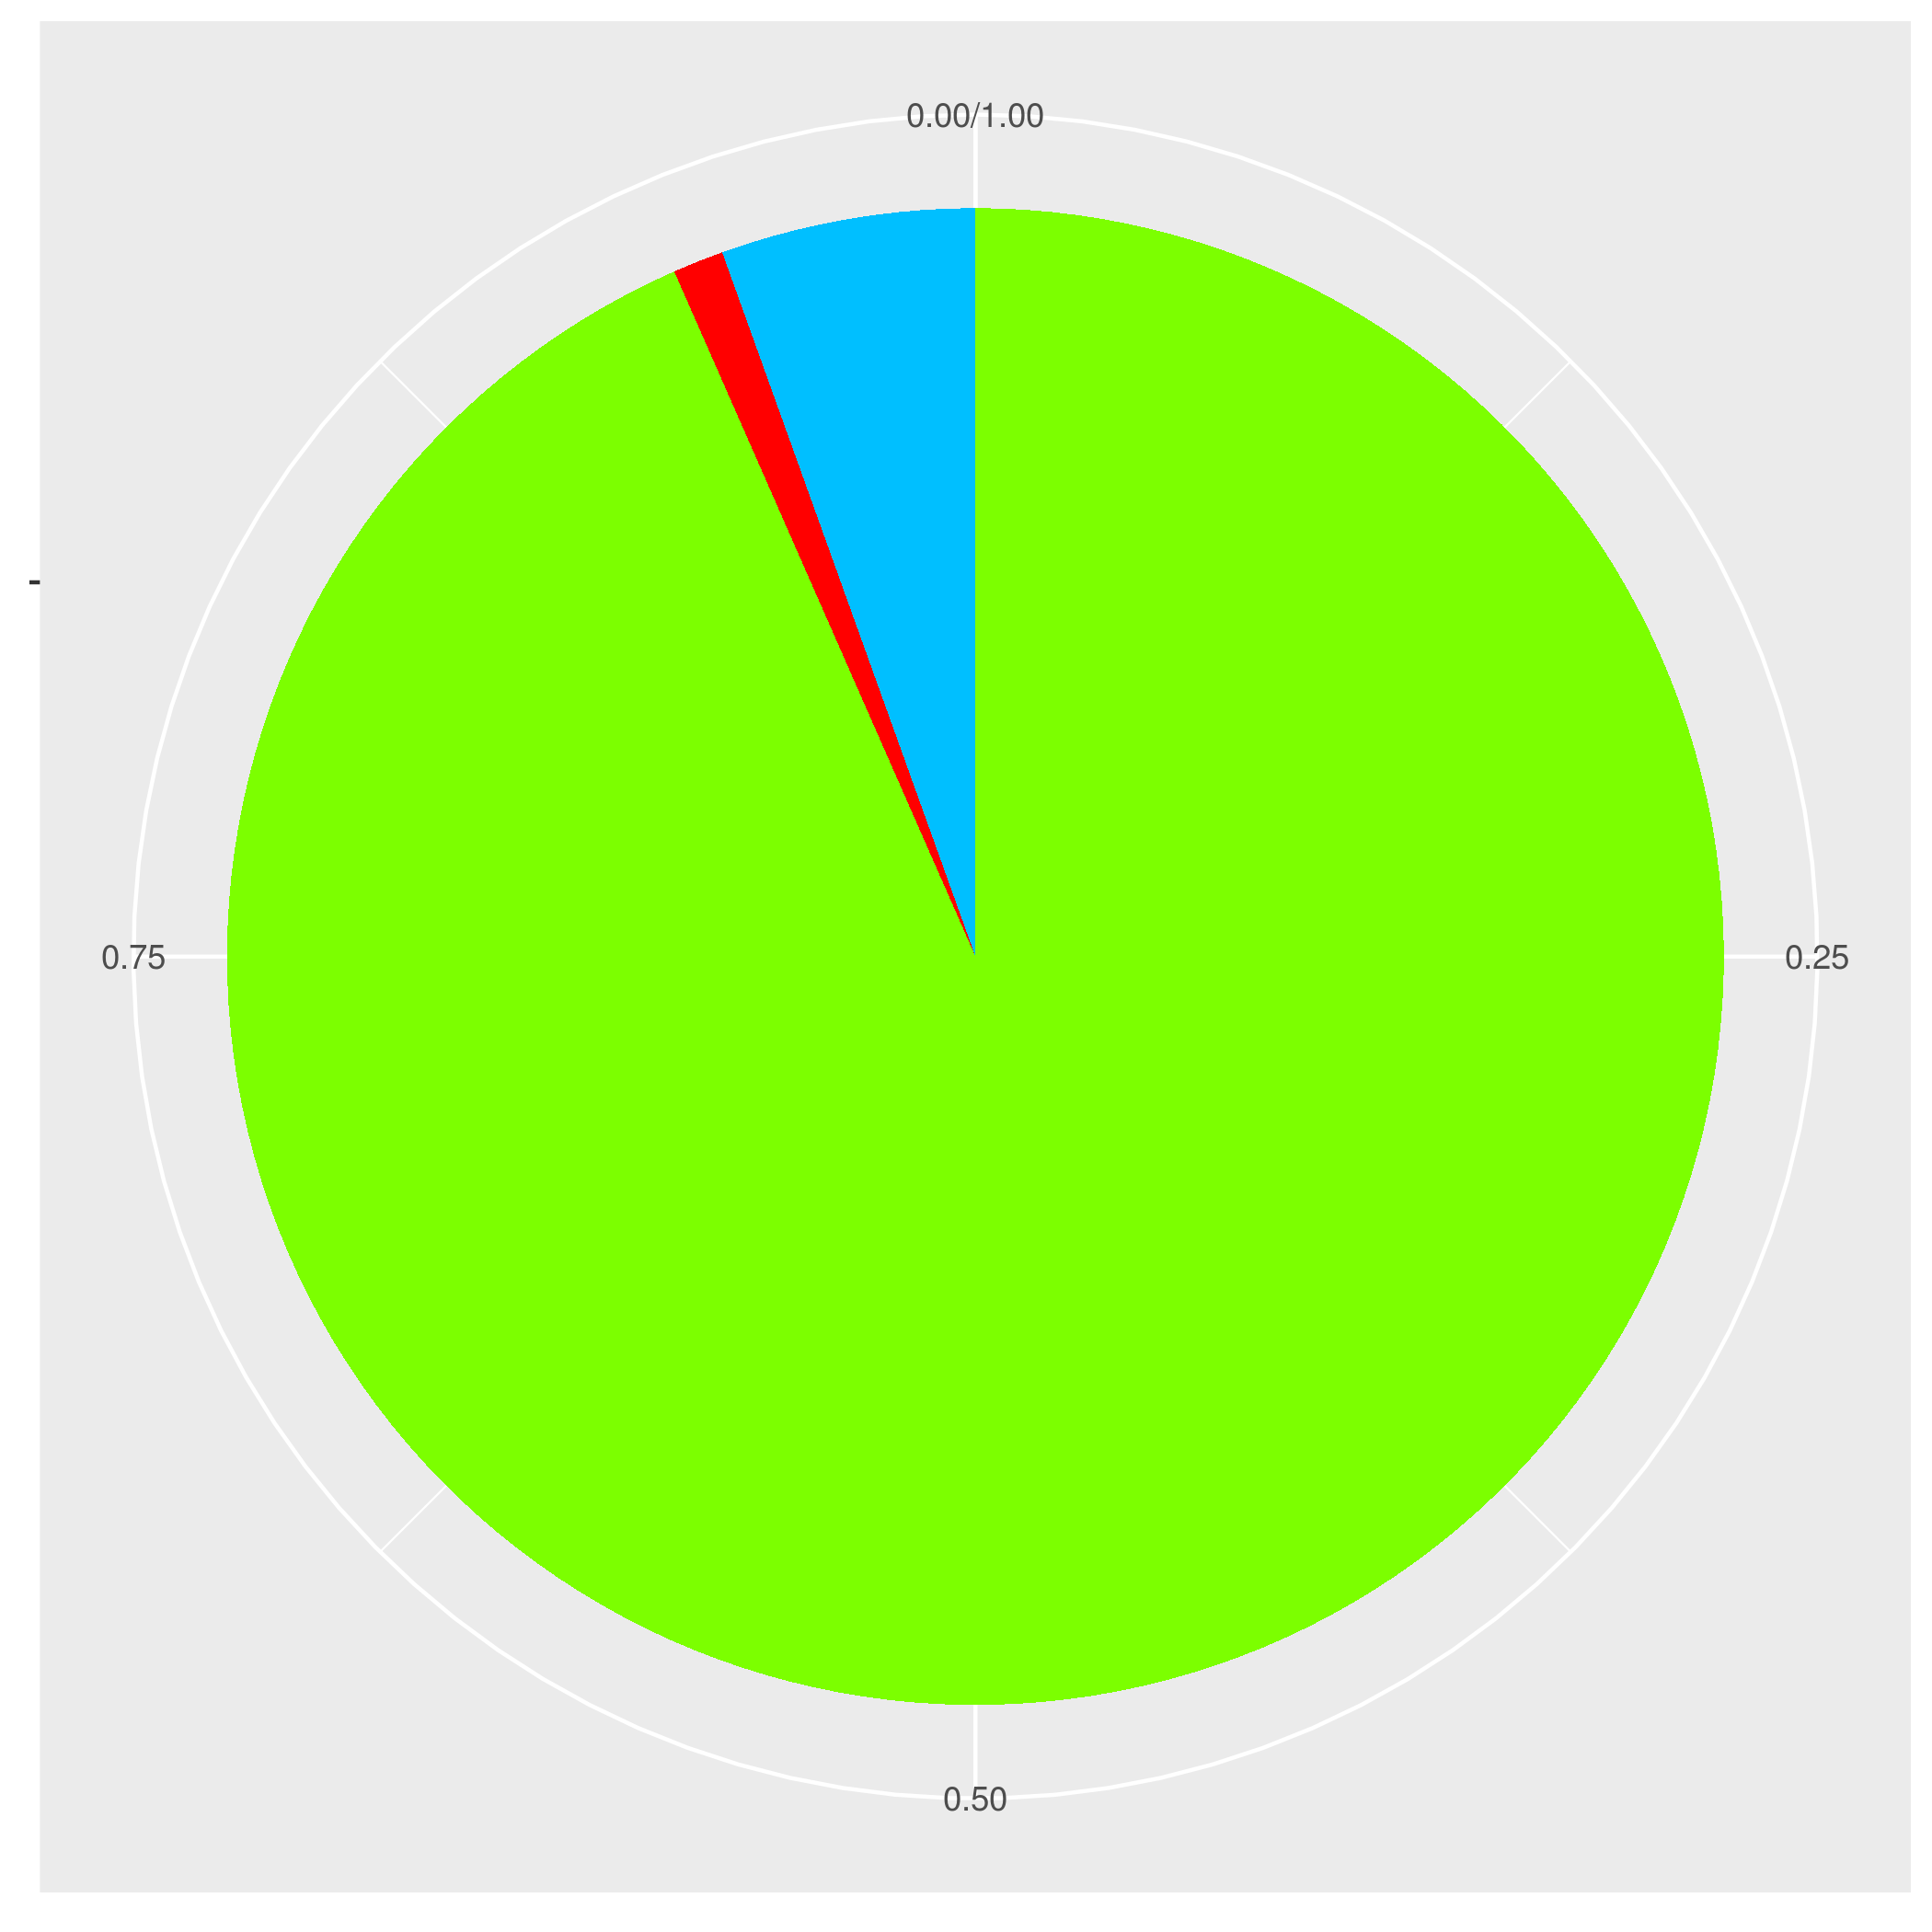
\includegraphics[width=.25\columnwidth]{T40I10D100K.dat/riondato-c1.png}
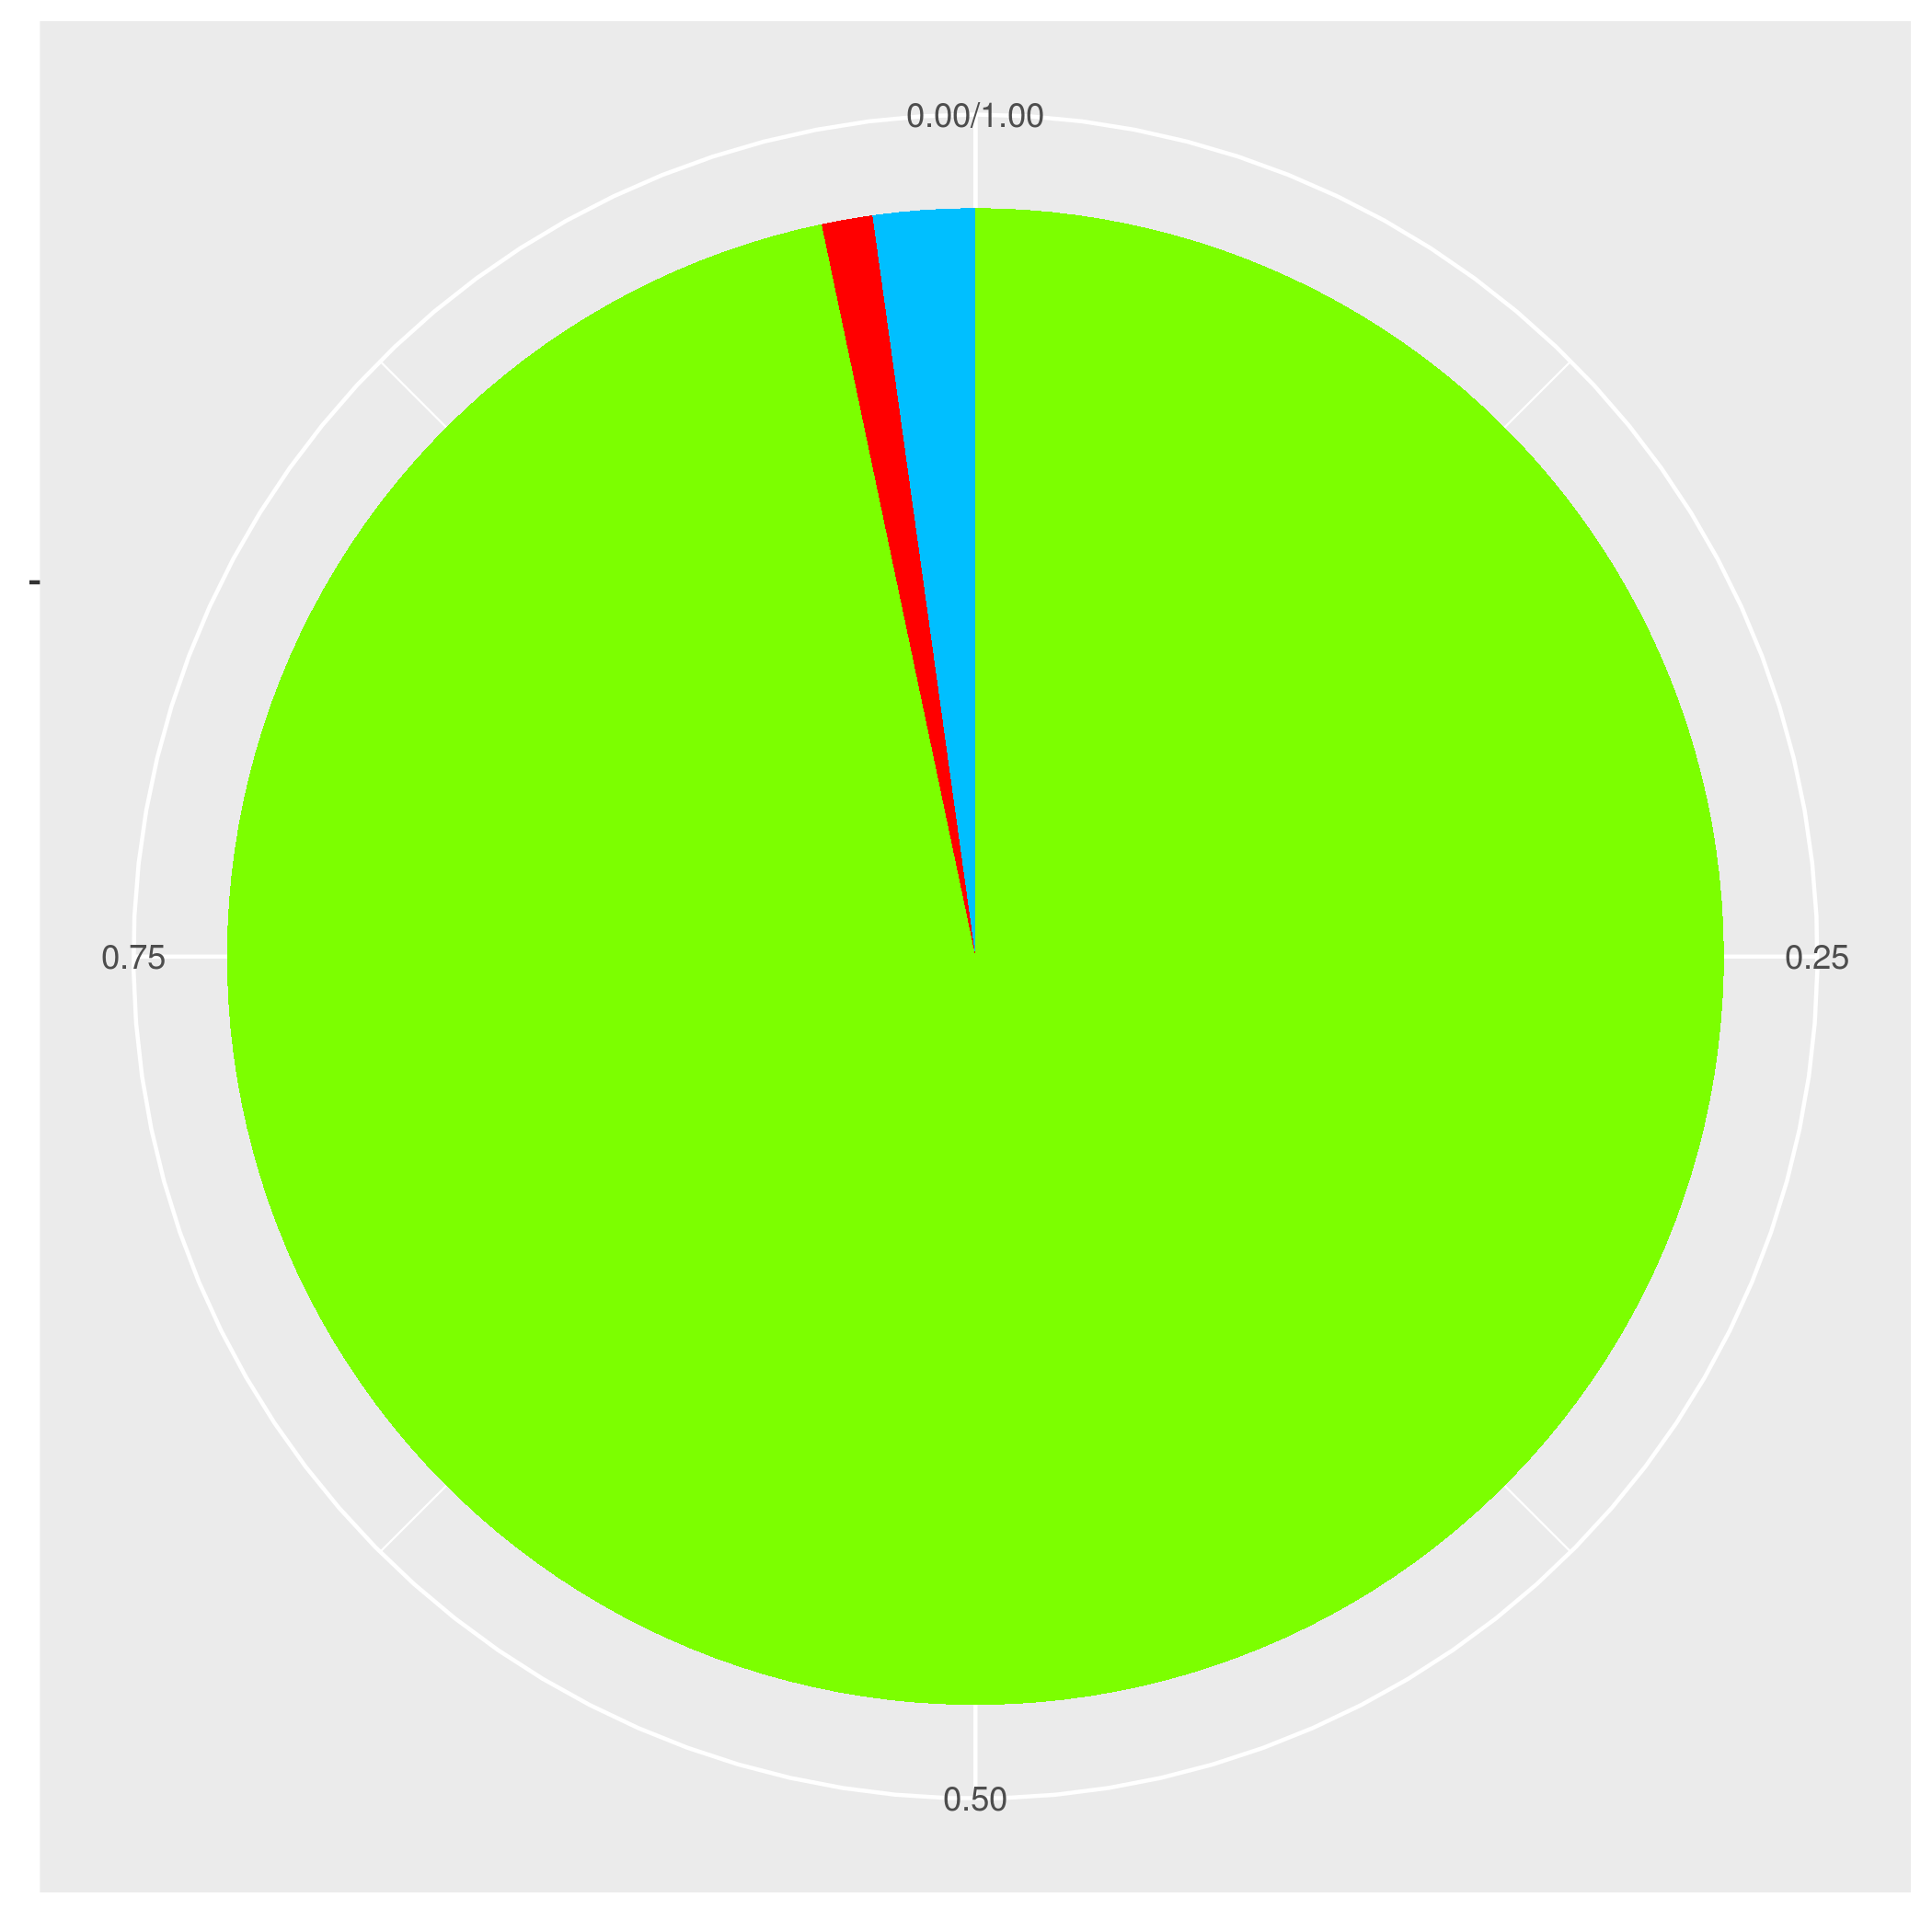
\includegraphics[width=.25\columnwidth]{T40I10D100K.dat/riondato-c2.png}
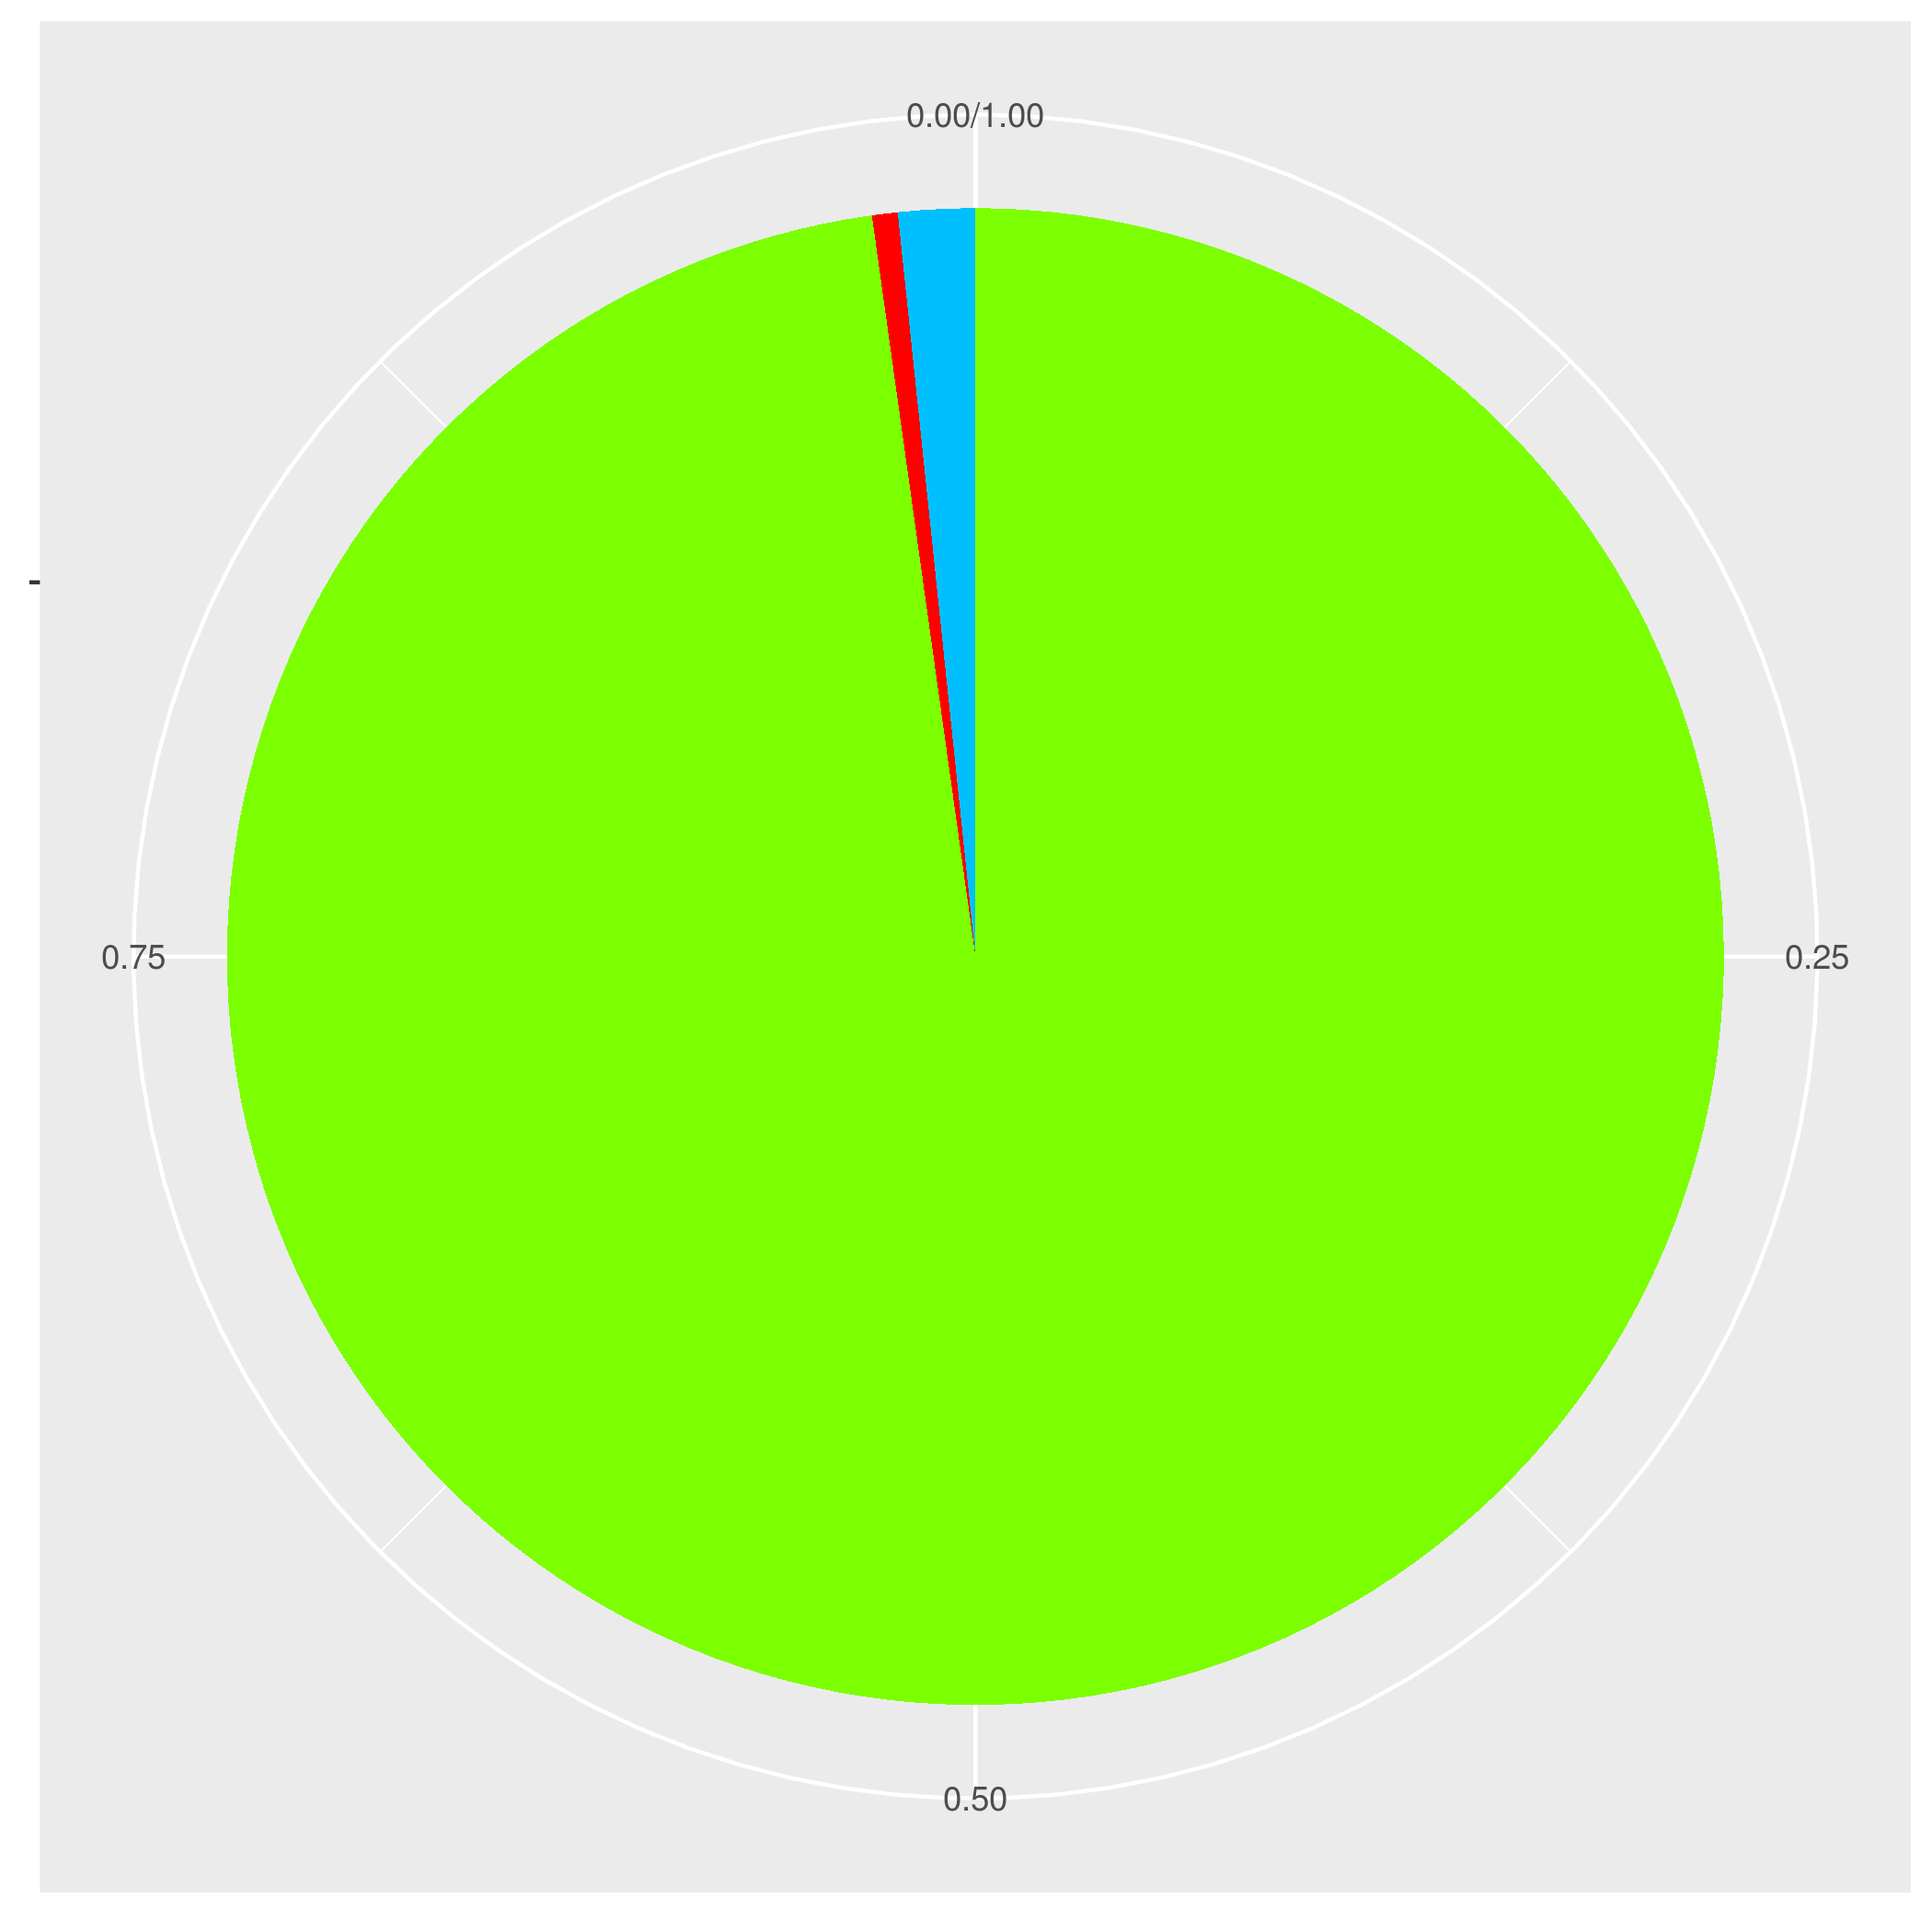
\includegraphics[width=.25\columnwidth]{T40I10D100K.dat/riondato-c3.png}\\
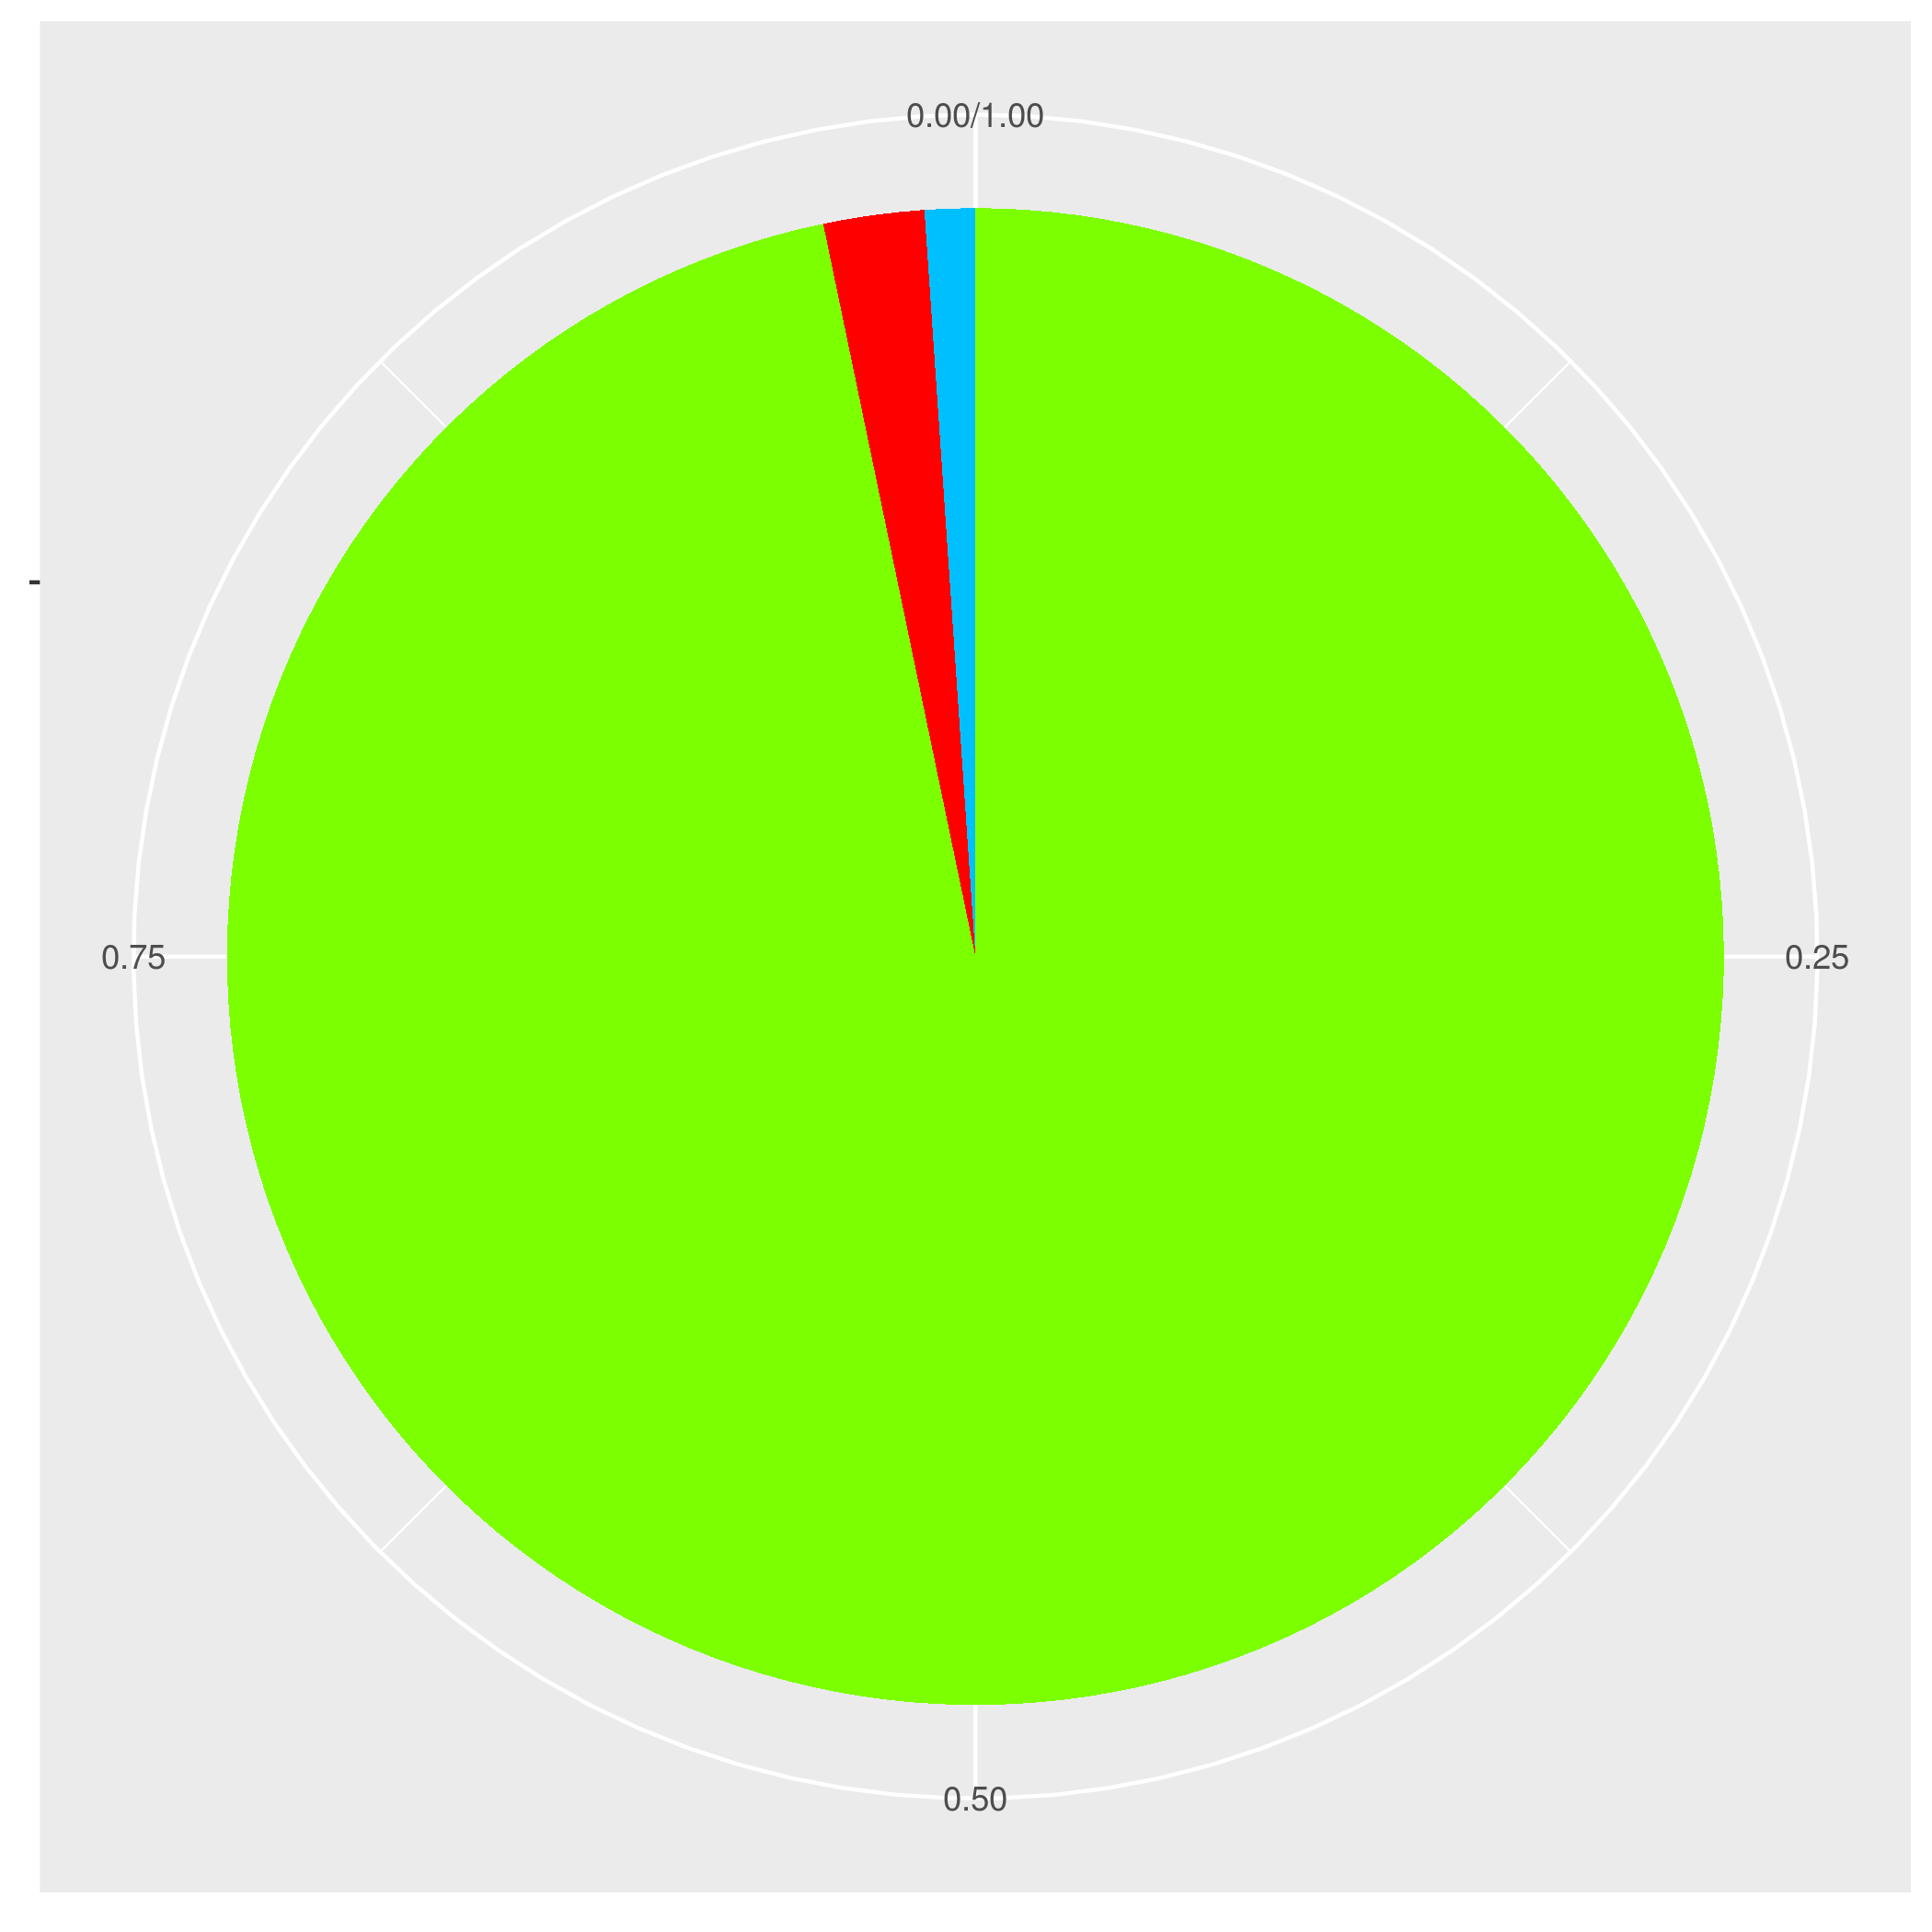
\includegraphics[width=.25\columnwidth]{T40I10D100K.dat/riondato-c4.png}
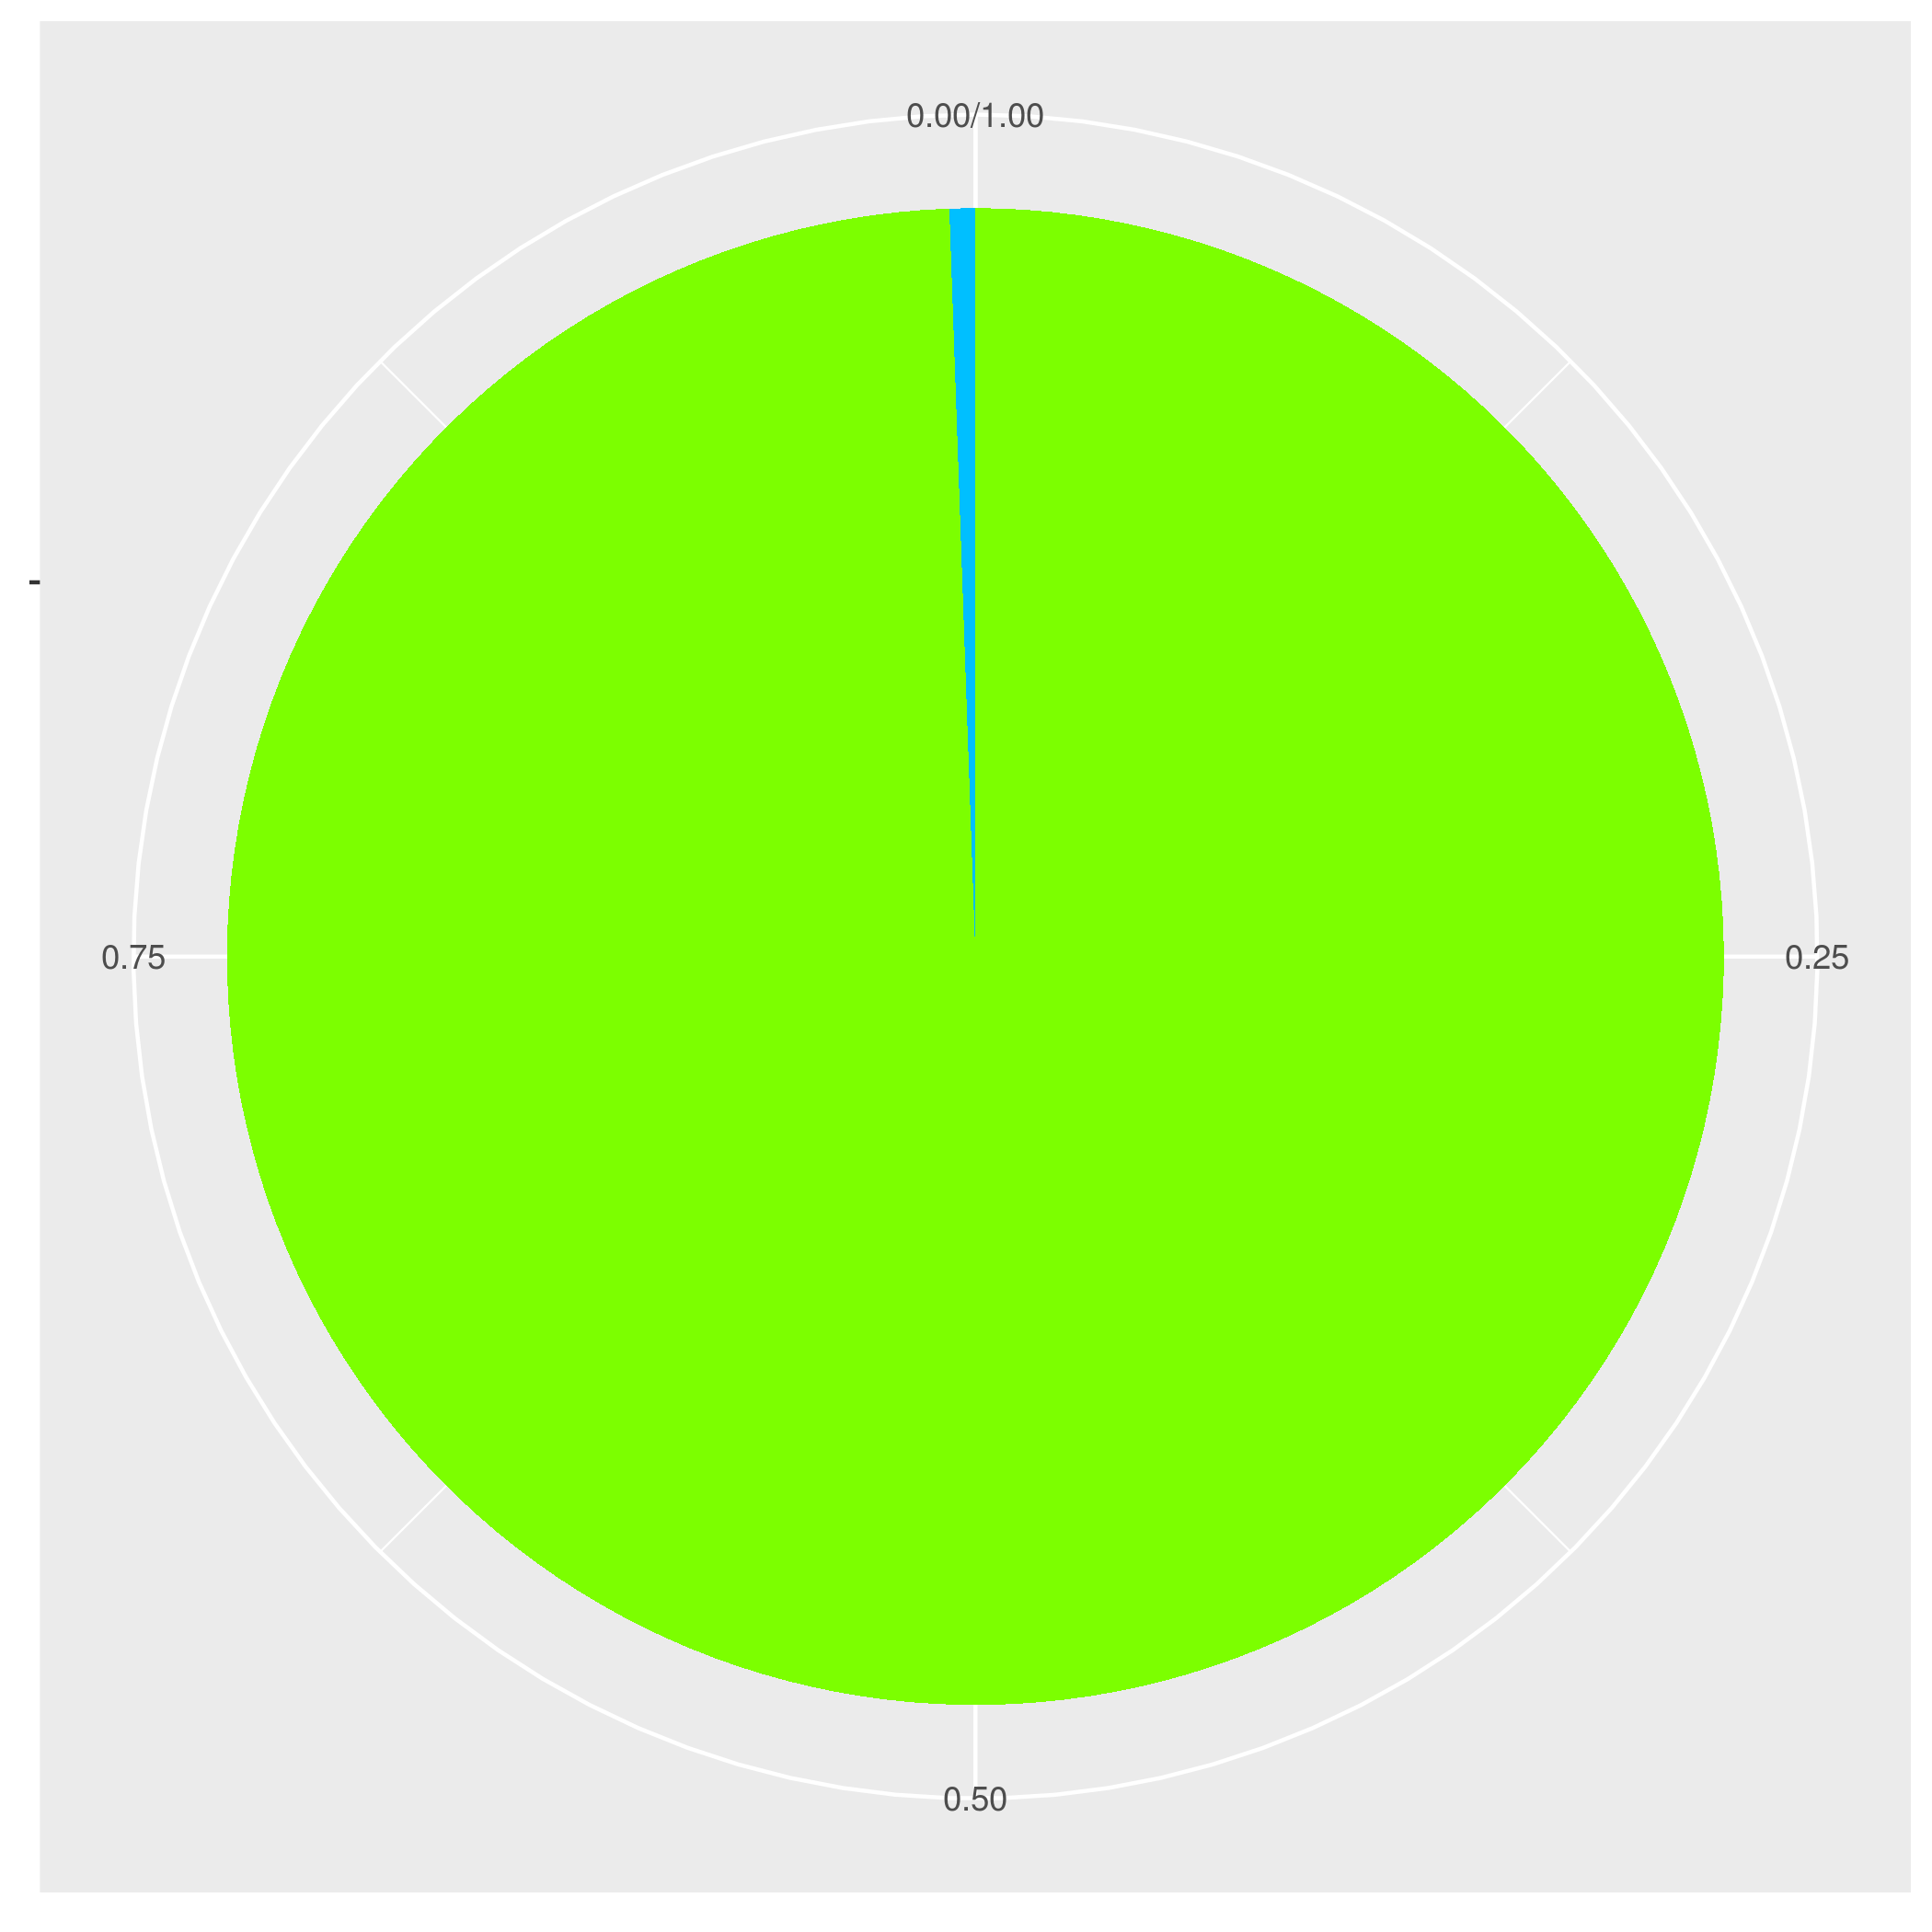
\includegraphics[width=.25\columnwidth]{T40I10D100K.dat/riondato-c5.png}
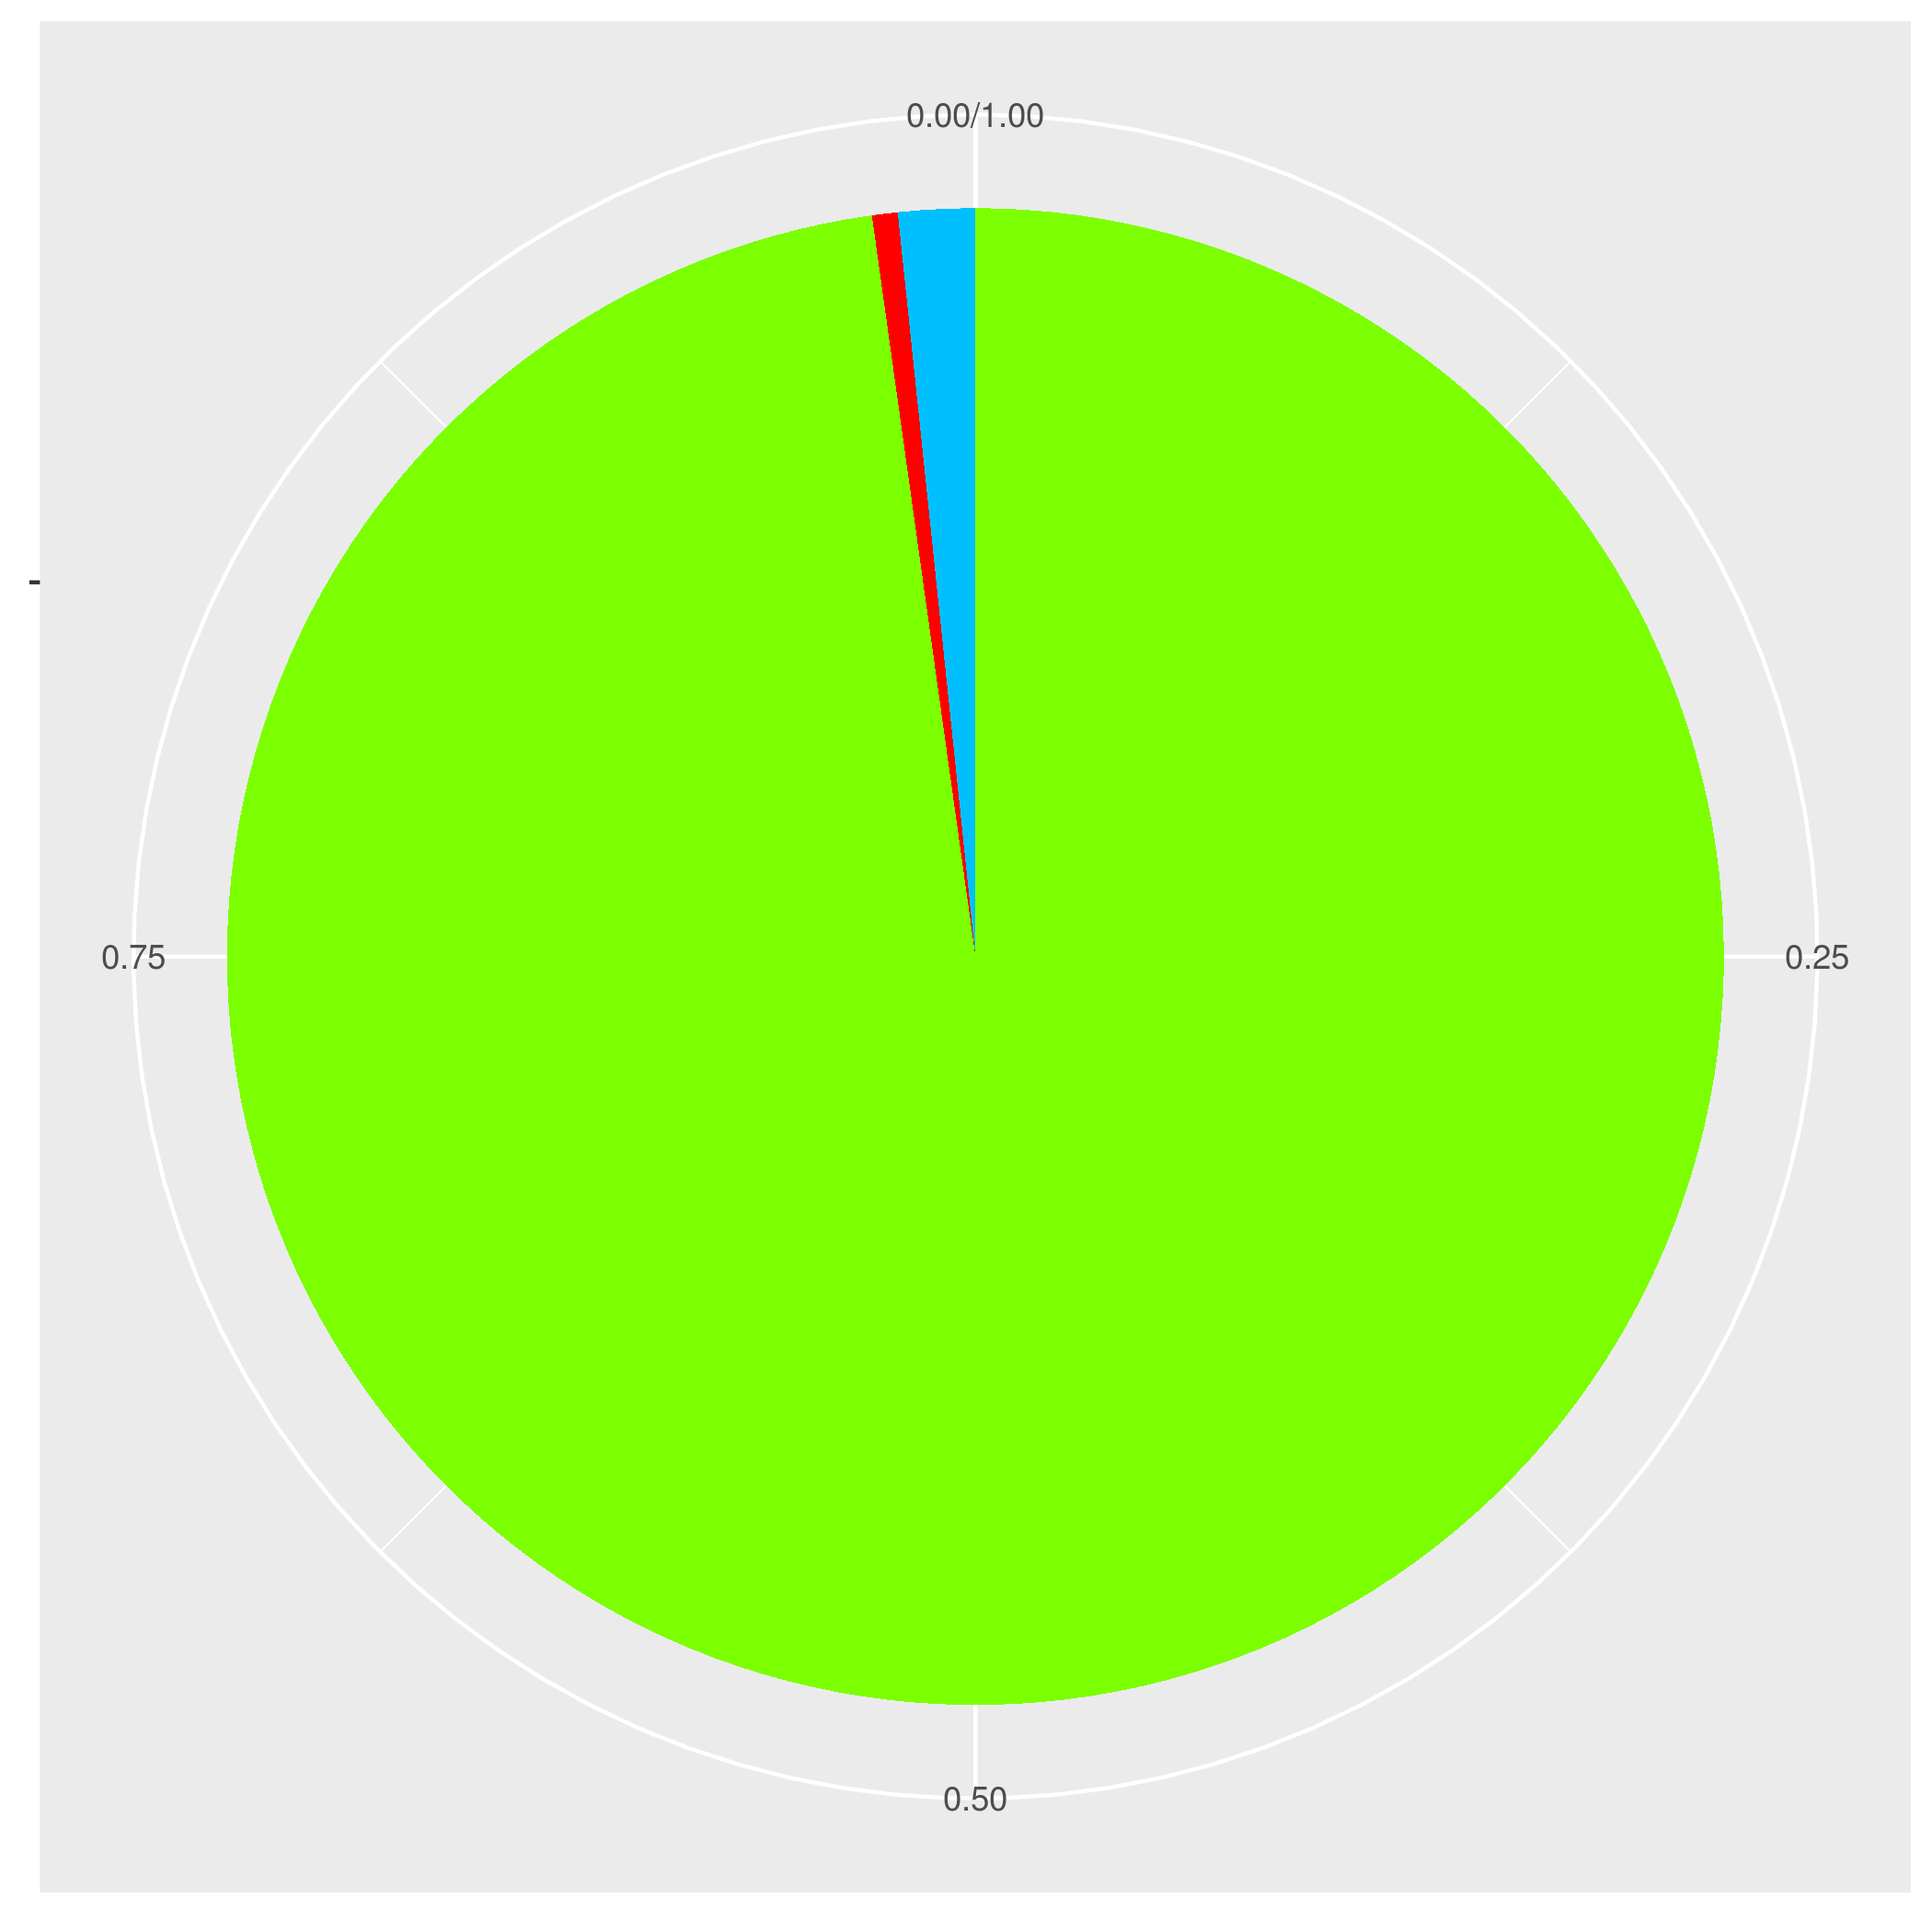
\includegraphics[width=.25\columnwidth]{T40I10D100K.dat/riondato-c6.png}
\end{figure}

It is observable across all charts, that the stricter the thresholds $\epsilon$ and $\delta$, the better the results (i.e. more true positives, less false answers).

The clear outlier here is the impact of lowering the threshold in Toivonen's approach, since this entails retrieving many itemsets that are not indeed frequent (i.e. false-positives). Of course, the same effect is aided by the (much smaller) required sample sizes. The only reasonable results in Toivonen appear when we set a stricter approximation error $\epsilon$, which consequently requires larger samples.

On the other hand, Riondato's method exhibits a stable and consistent behaviour across configurations, with results getting increasingly better towards stricter parameters.

We can now see the precision and recall metrics, to get a concise overview of the accuracy of the two methods. Below we depict the precision on the left and the recall on the right:

\begin{center}
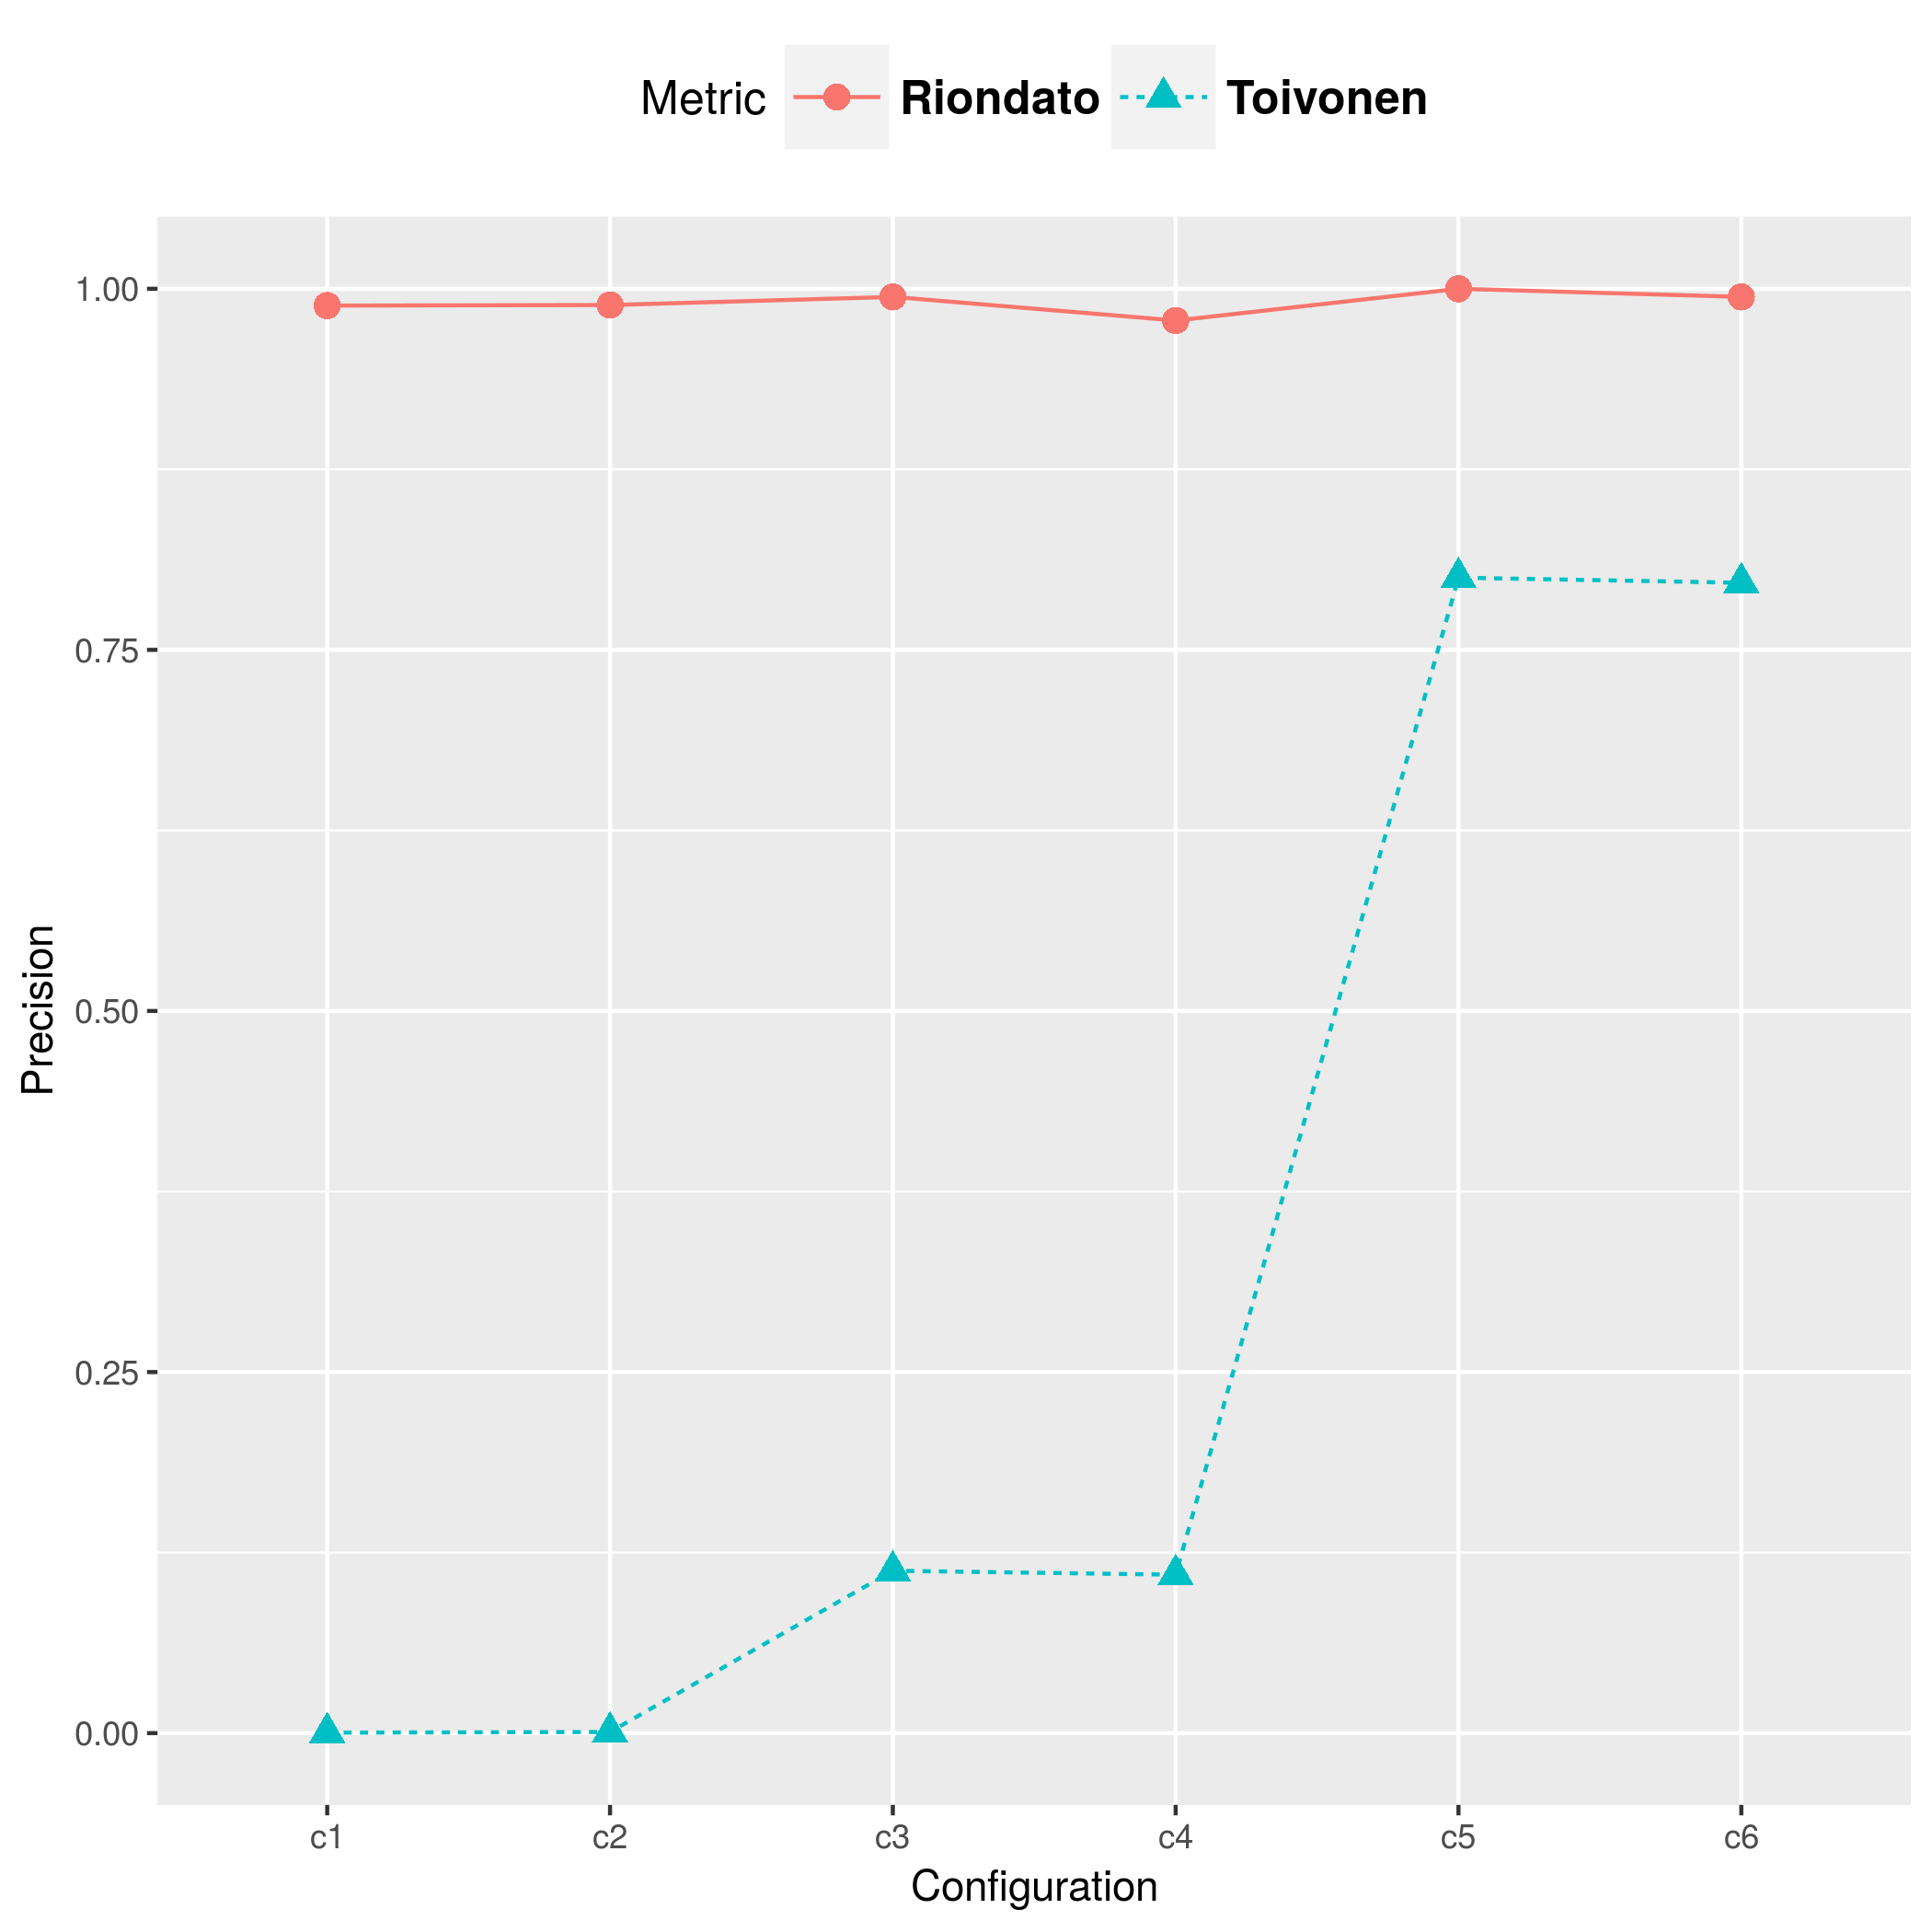
\includegraphics[width=.45\columnwidth]{T40I10D100K.dat/precision.png}
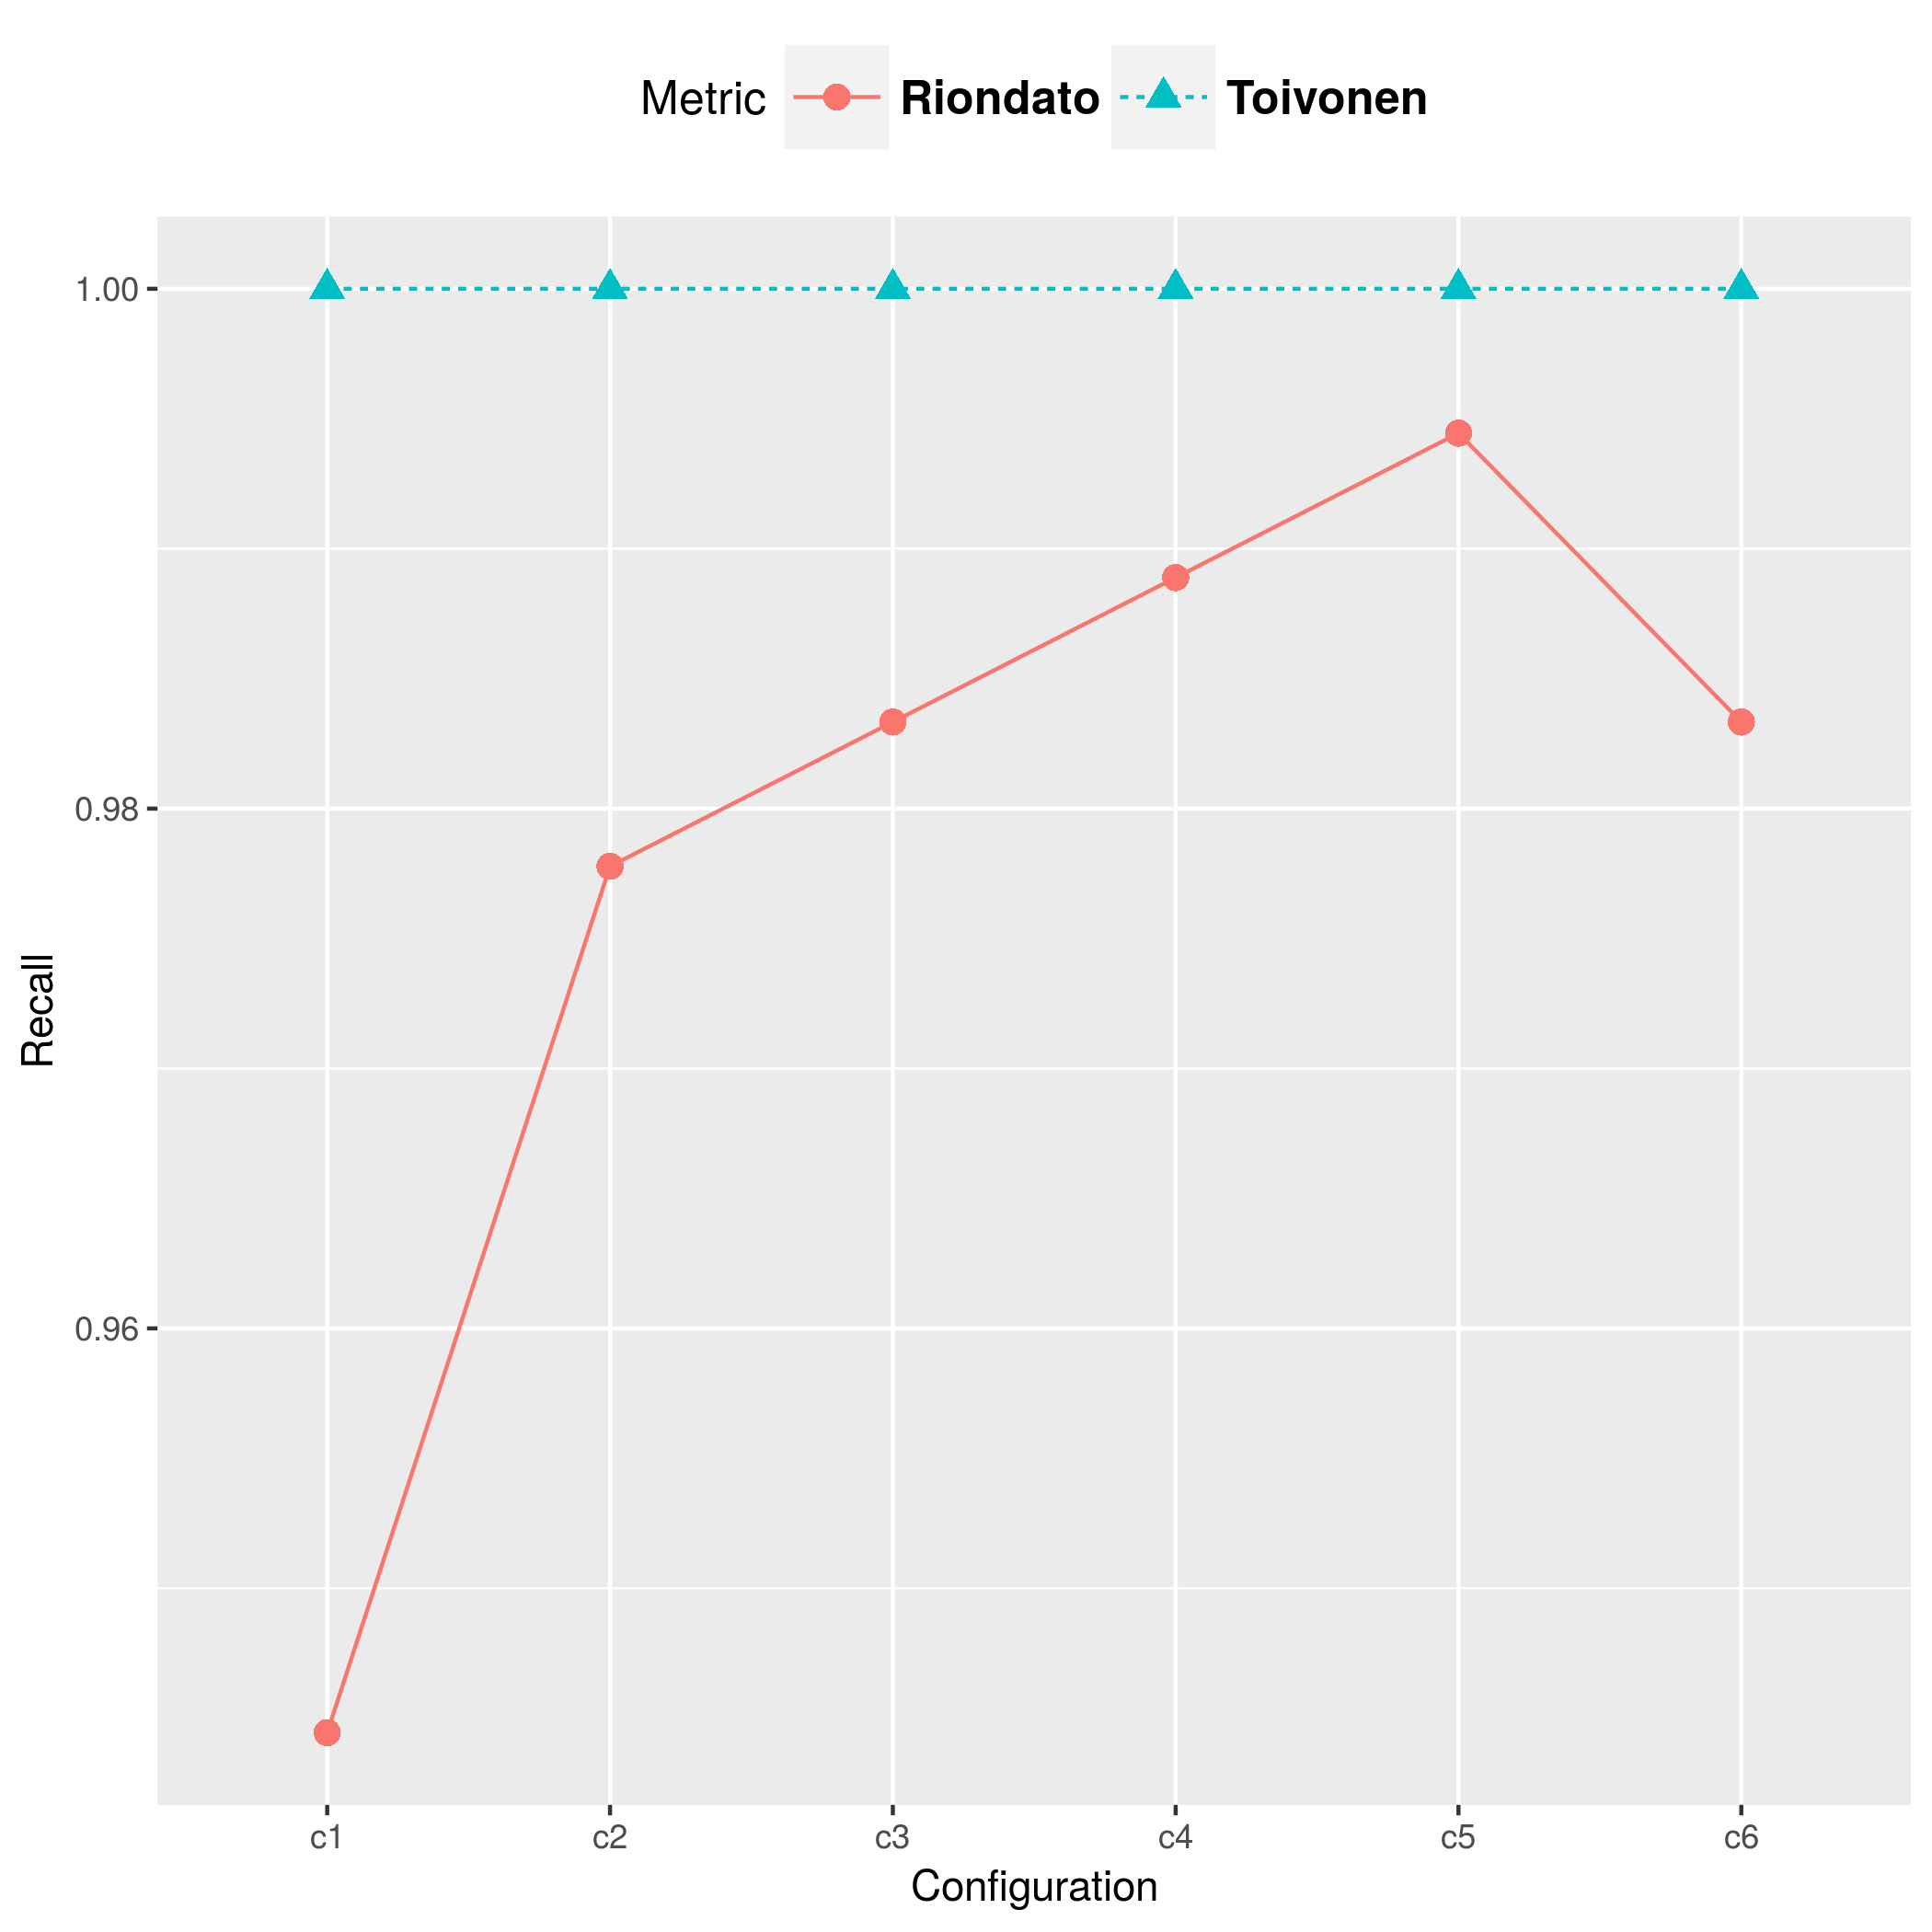
\includegraphics[width=.45\columnwidth]{T40I10D100K.dat/recall.png}
\end{center}

Regarding precision, we observe that Riondato's approach has optimal results in all parameter settings, while Toivonen's is completely inaccurate in the looser settings. In stricter settings, due to larger required samples, Toivonen gets reasonably accurate, but still lower than the other method.

Regarding recall, Toivonen's method is, surprisingly, consistently perfect. This means, essentially, that it managed to find almost all frequent itemsets with a much smaller sample. We can claim that Toivonen's approach is much more "productive", meaning that it retrieves \textit{too many} itemsets, some irrelevant and some not. Riondato is again consistent with previous results, being more accurate when we go to stricter configurations.

\subsubsection{Frequency error}
While precision and recall are well-established metrics for model accuracy, they do not tell us more about the nature of false answers (positive/negative). In other words, we would like to know how further a false-answer's support is from the real one.

To achieve this, we measure the error of the frequency estimation, which is a more fine-grained metric of accuracy.
\begin{figure}[h!]
\centering
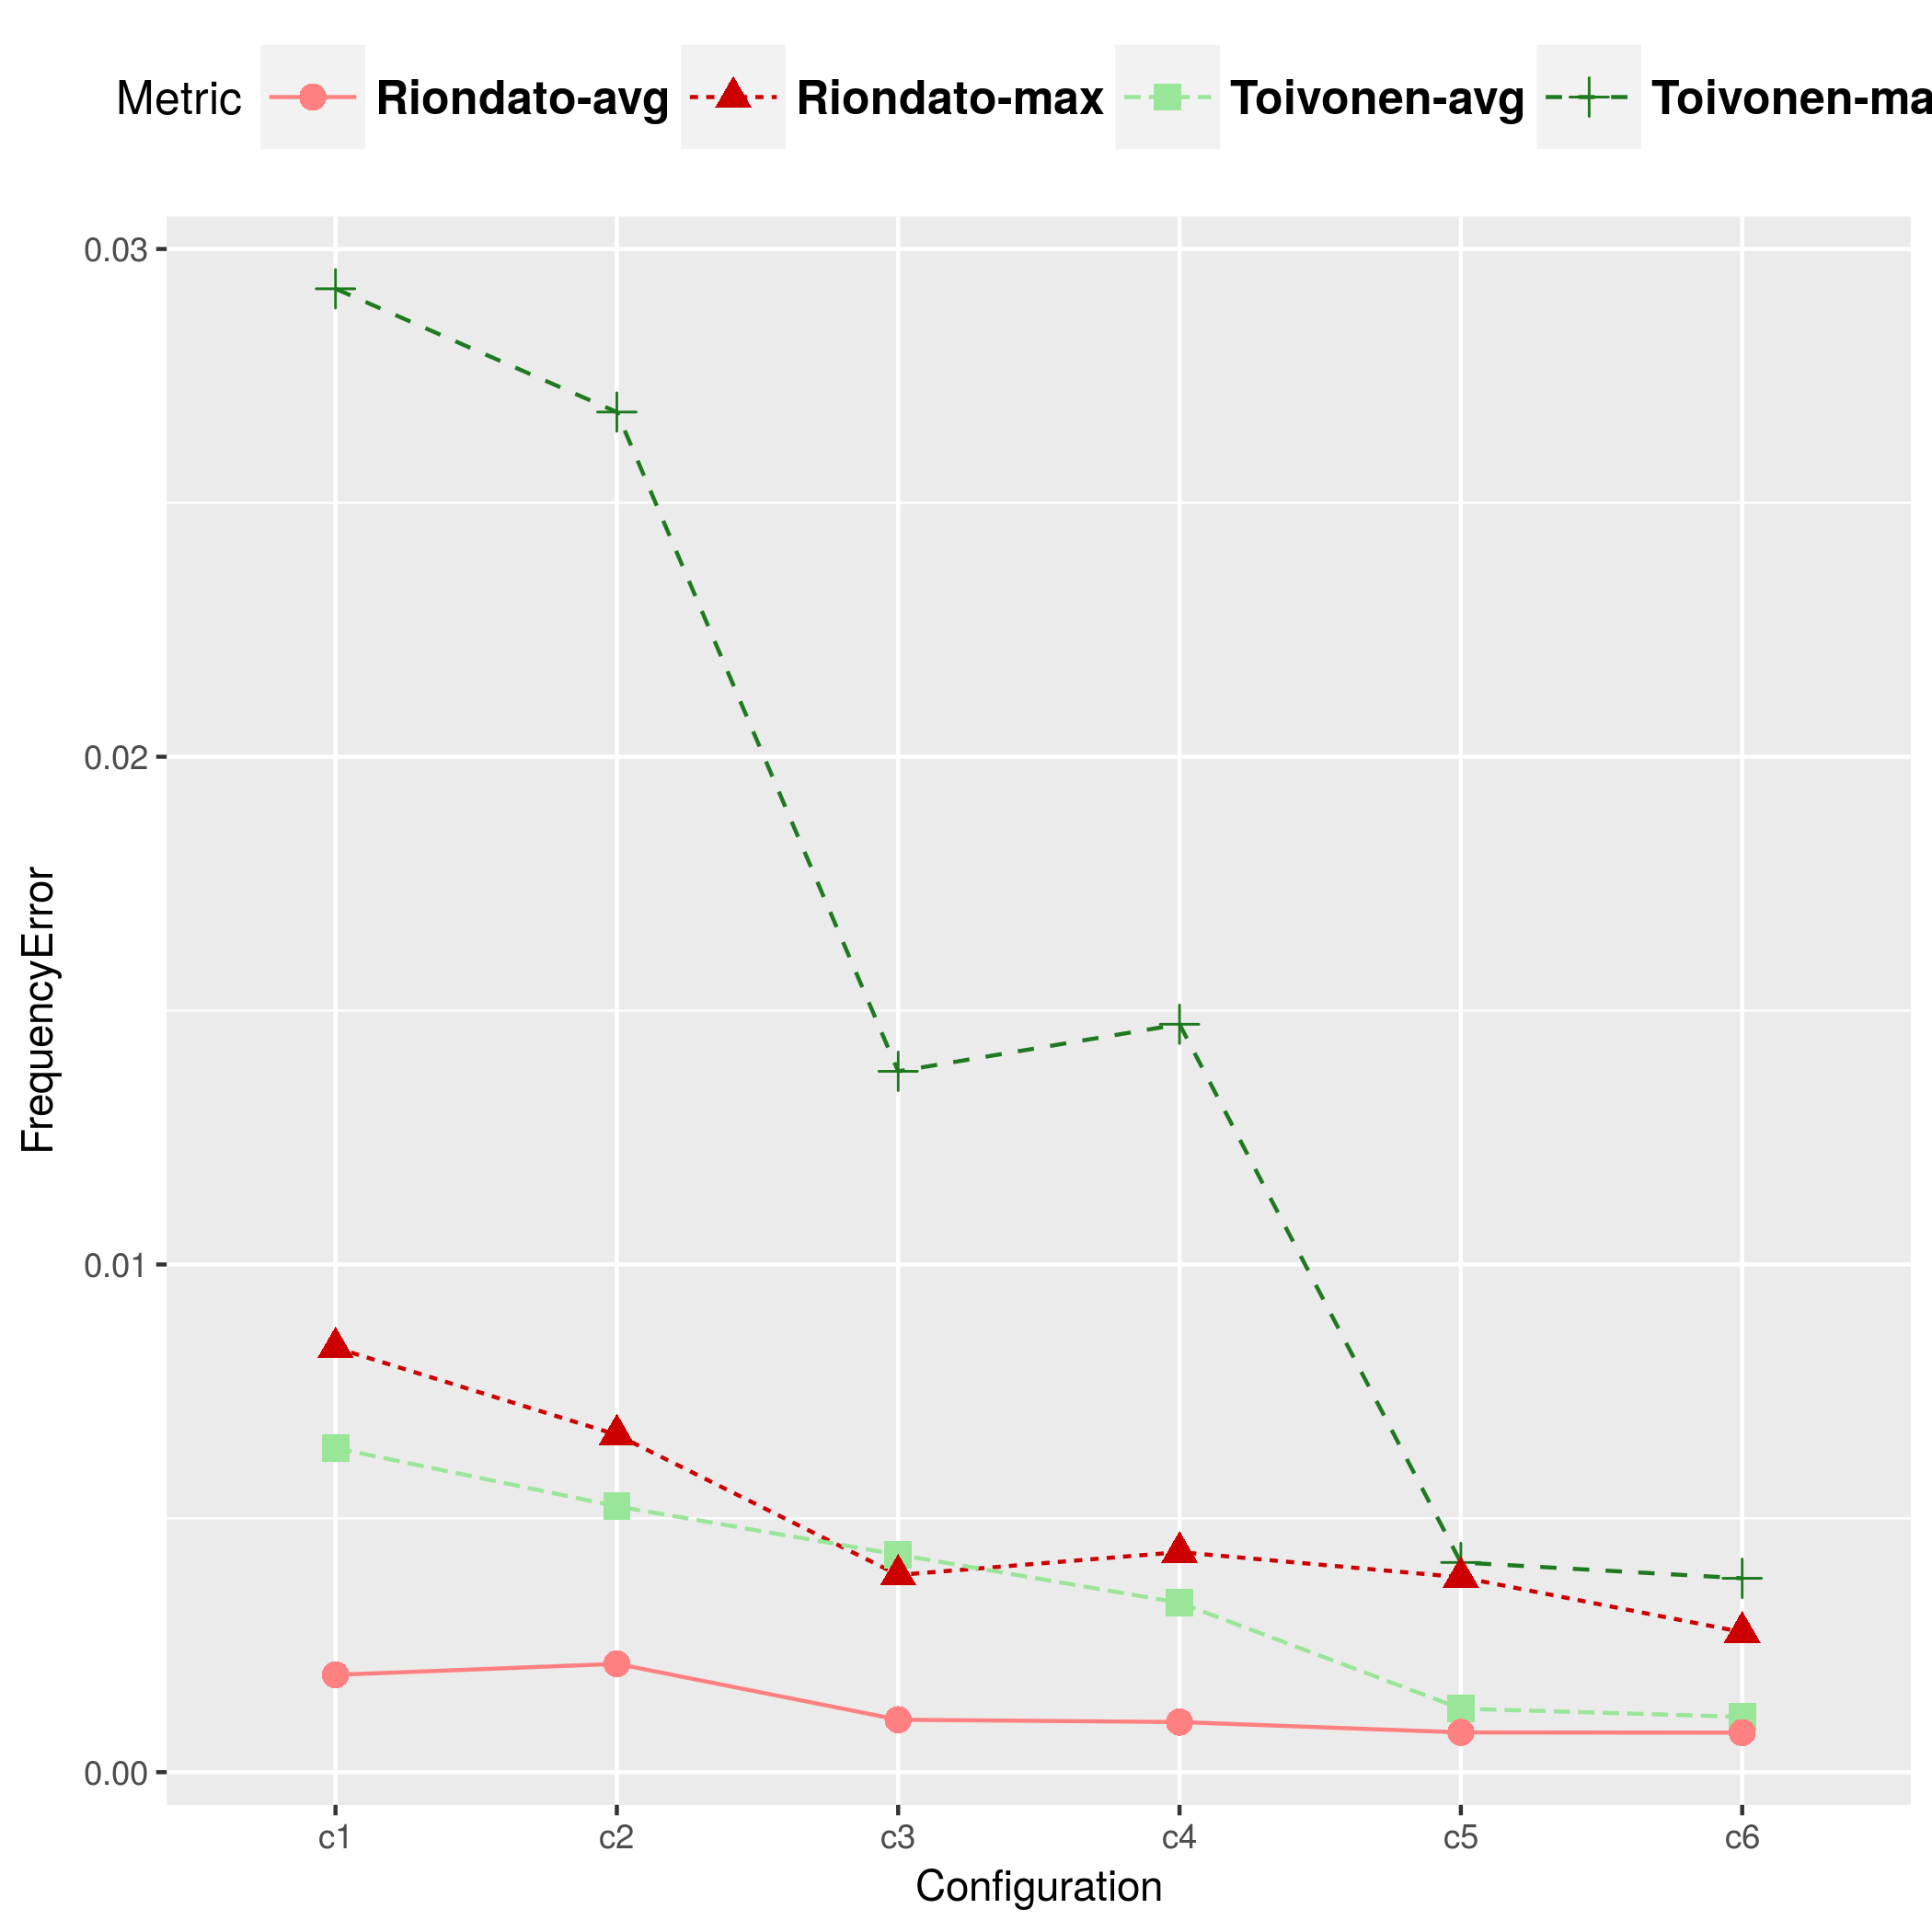
\includegraphics[width=.7\columnwidth]{T40I10D100K.dat/freq.png}
\end{figure}
As we move to stricter configurations, both maximum and averages errors of both methods are very low. Across all settings, we observe that Riondato's approach consistently gives smaller errors. In looser settings, we notice that Toivonen's approach shows very large maximum errors.

\subsection{Dataset II: kosarak}
We now present the results on a real dataset, namely one consisting of click-stream data of a news portal. Its size is very large ($|\D| \simeq 1.000.000$) and has a much larger d-bound than the artificial dataset ($443 >> 67$). This will inform us on whether the proposed techniques scale well with size.

We refrain from repeating observations already made in the artificial dataset, but rather emphasize issues of scalability.

\subsubsection{Sample sizes}
\begin{figure}[h!]
\centering
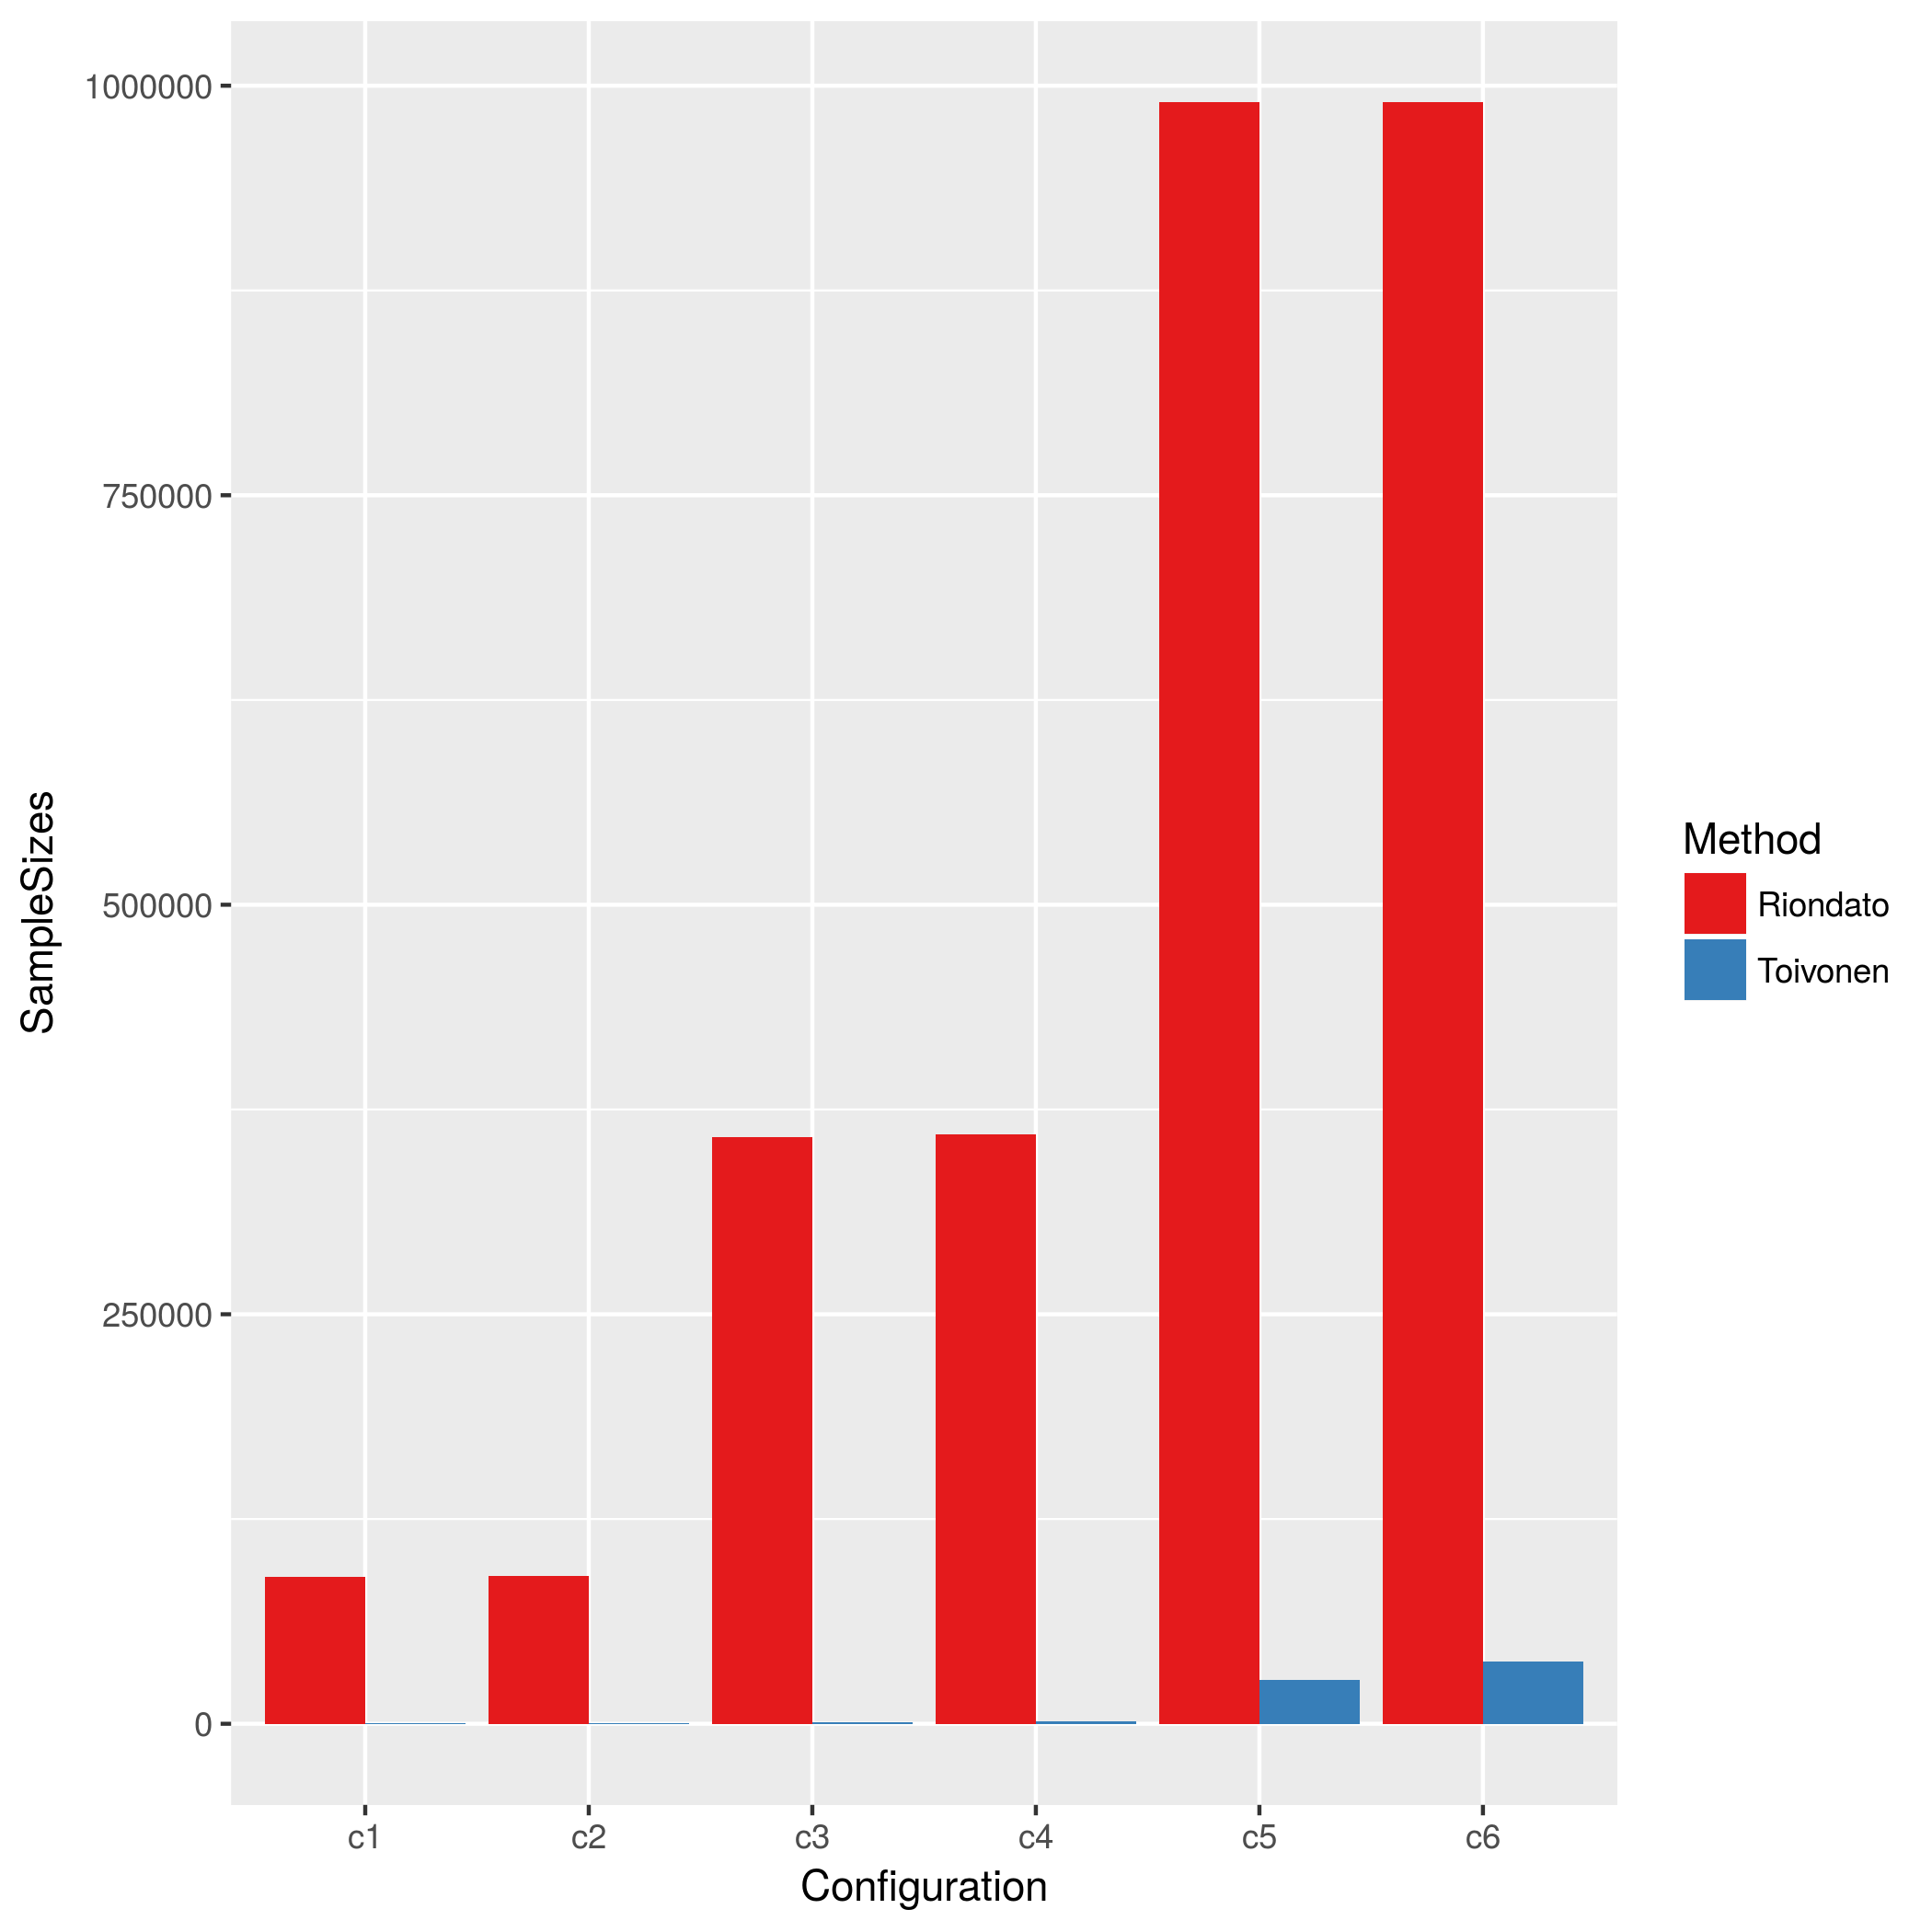
\includegraphics[width=.7\columnwidth]{kosarak.dat/sampleSizes.png}
\end{figure}
We still get much larger sample requirements from Riondato's bound, but now the difference is much higher, due to the larger d-bound of the dataset. The crucial observation we must make here is that Riondato's bound depends on the size and complexity of the dataset, while Toivonen's bound relies solely on the user-defined parameters. This hints on the fact that Riondato's method will scale much better as we move to larger datasets.

\subsubsection{Precision-Recall}
\begin{figure}[h!]
\centering
\caption*{Toivonen}
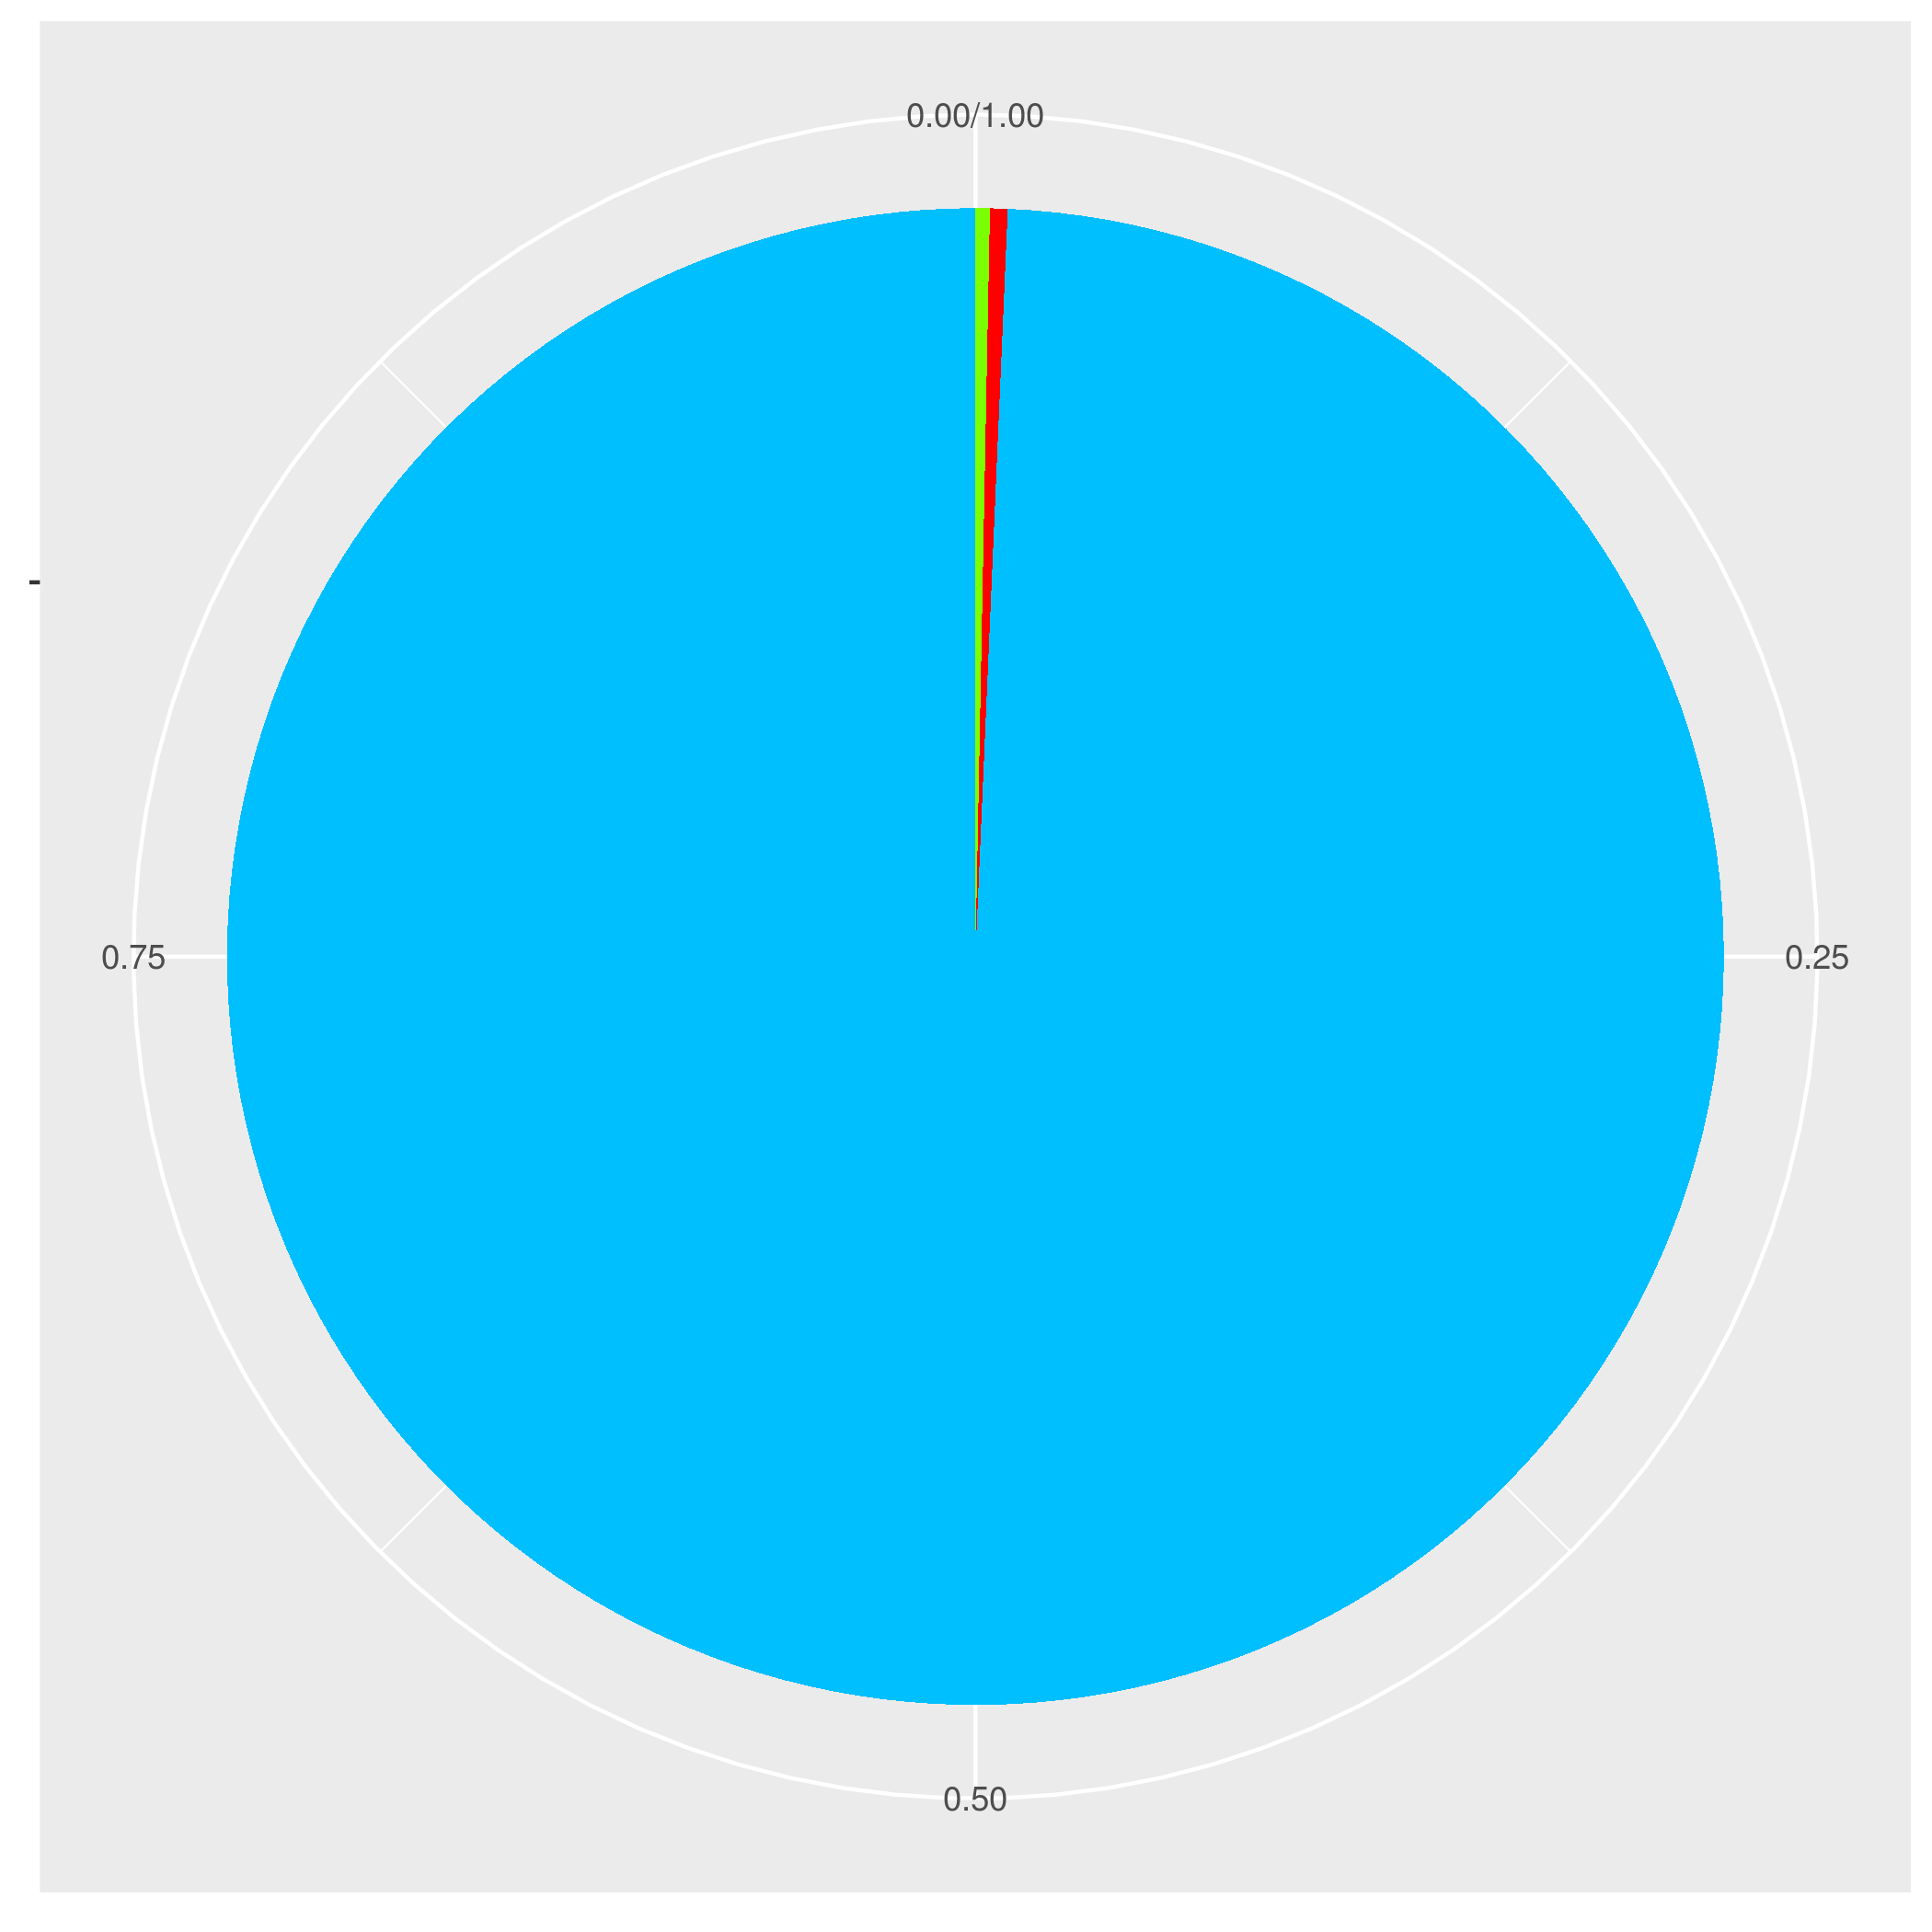
\includegraphics[width=.25\columnwidth]{kosarak.dat/toivonen-c1.png}
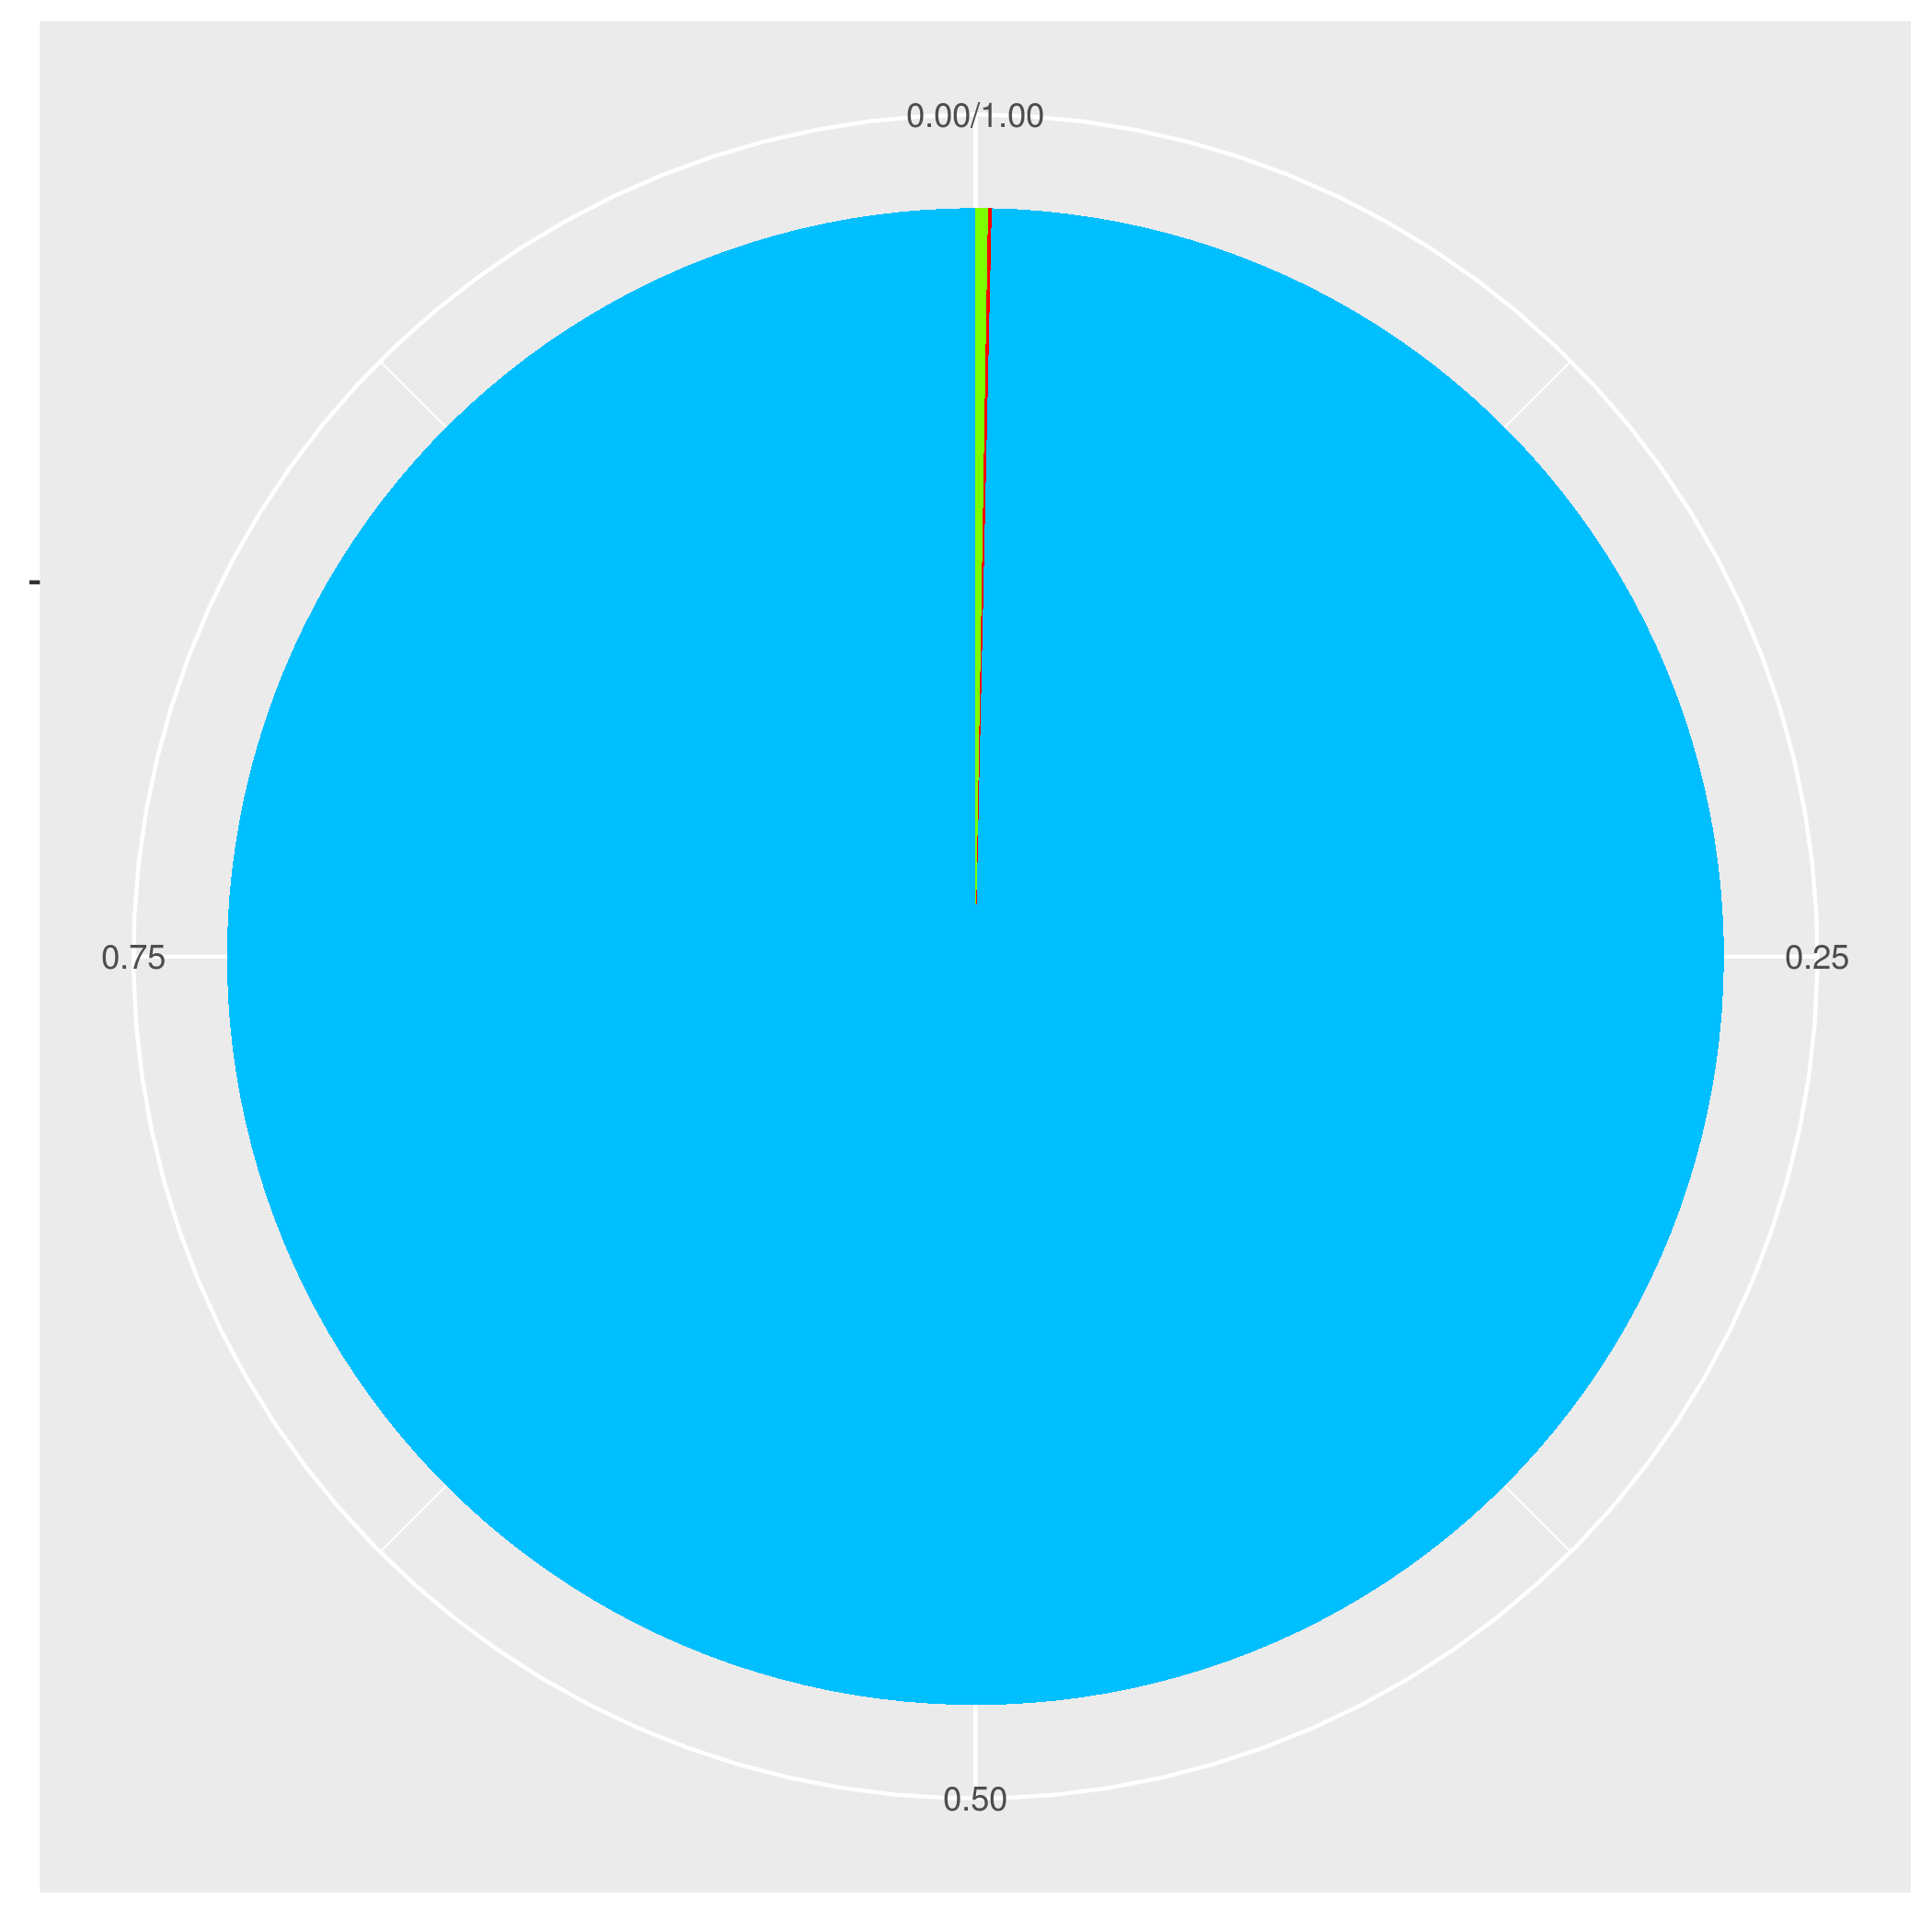
\includegraphics[width=.25\columnwidth]{kosarak.dat/toivonen-c2.png}
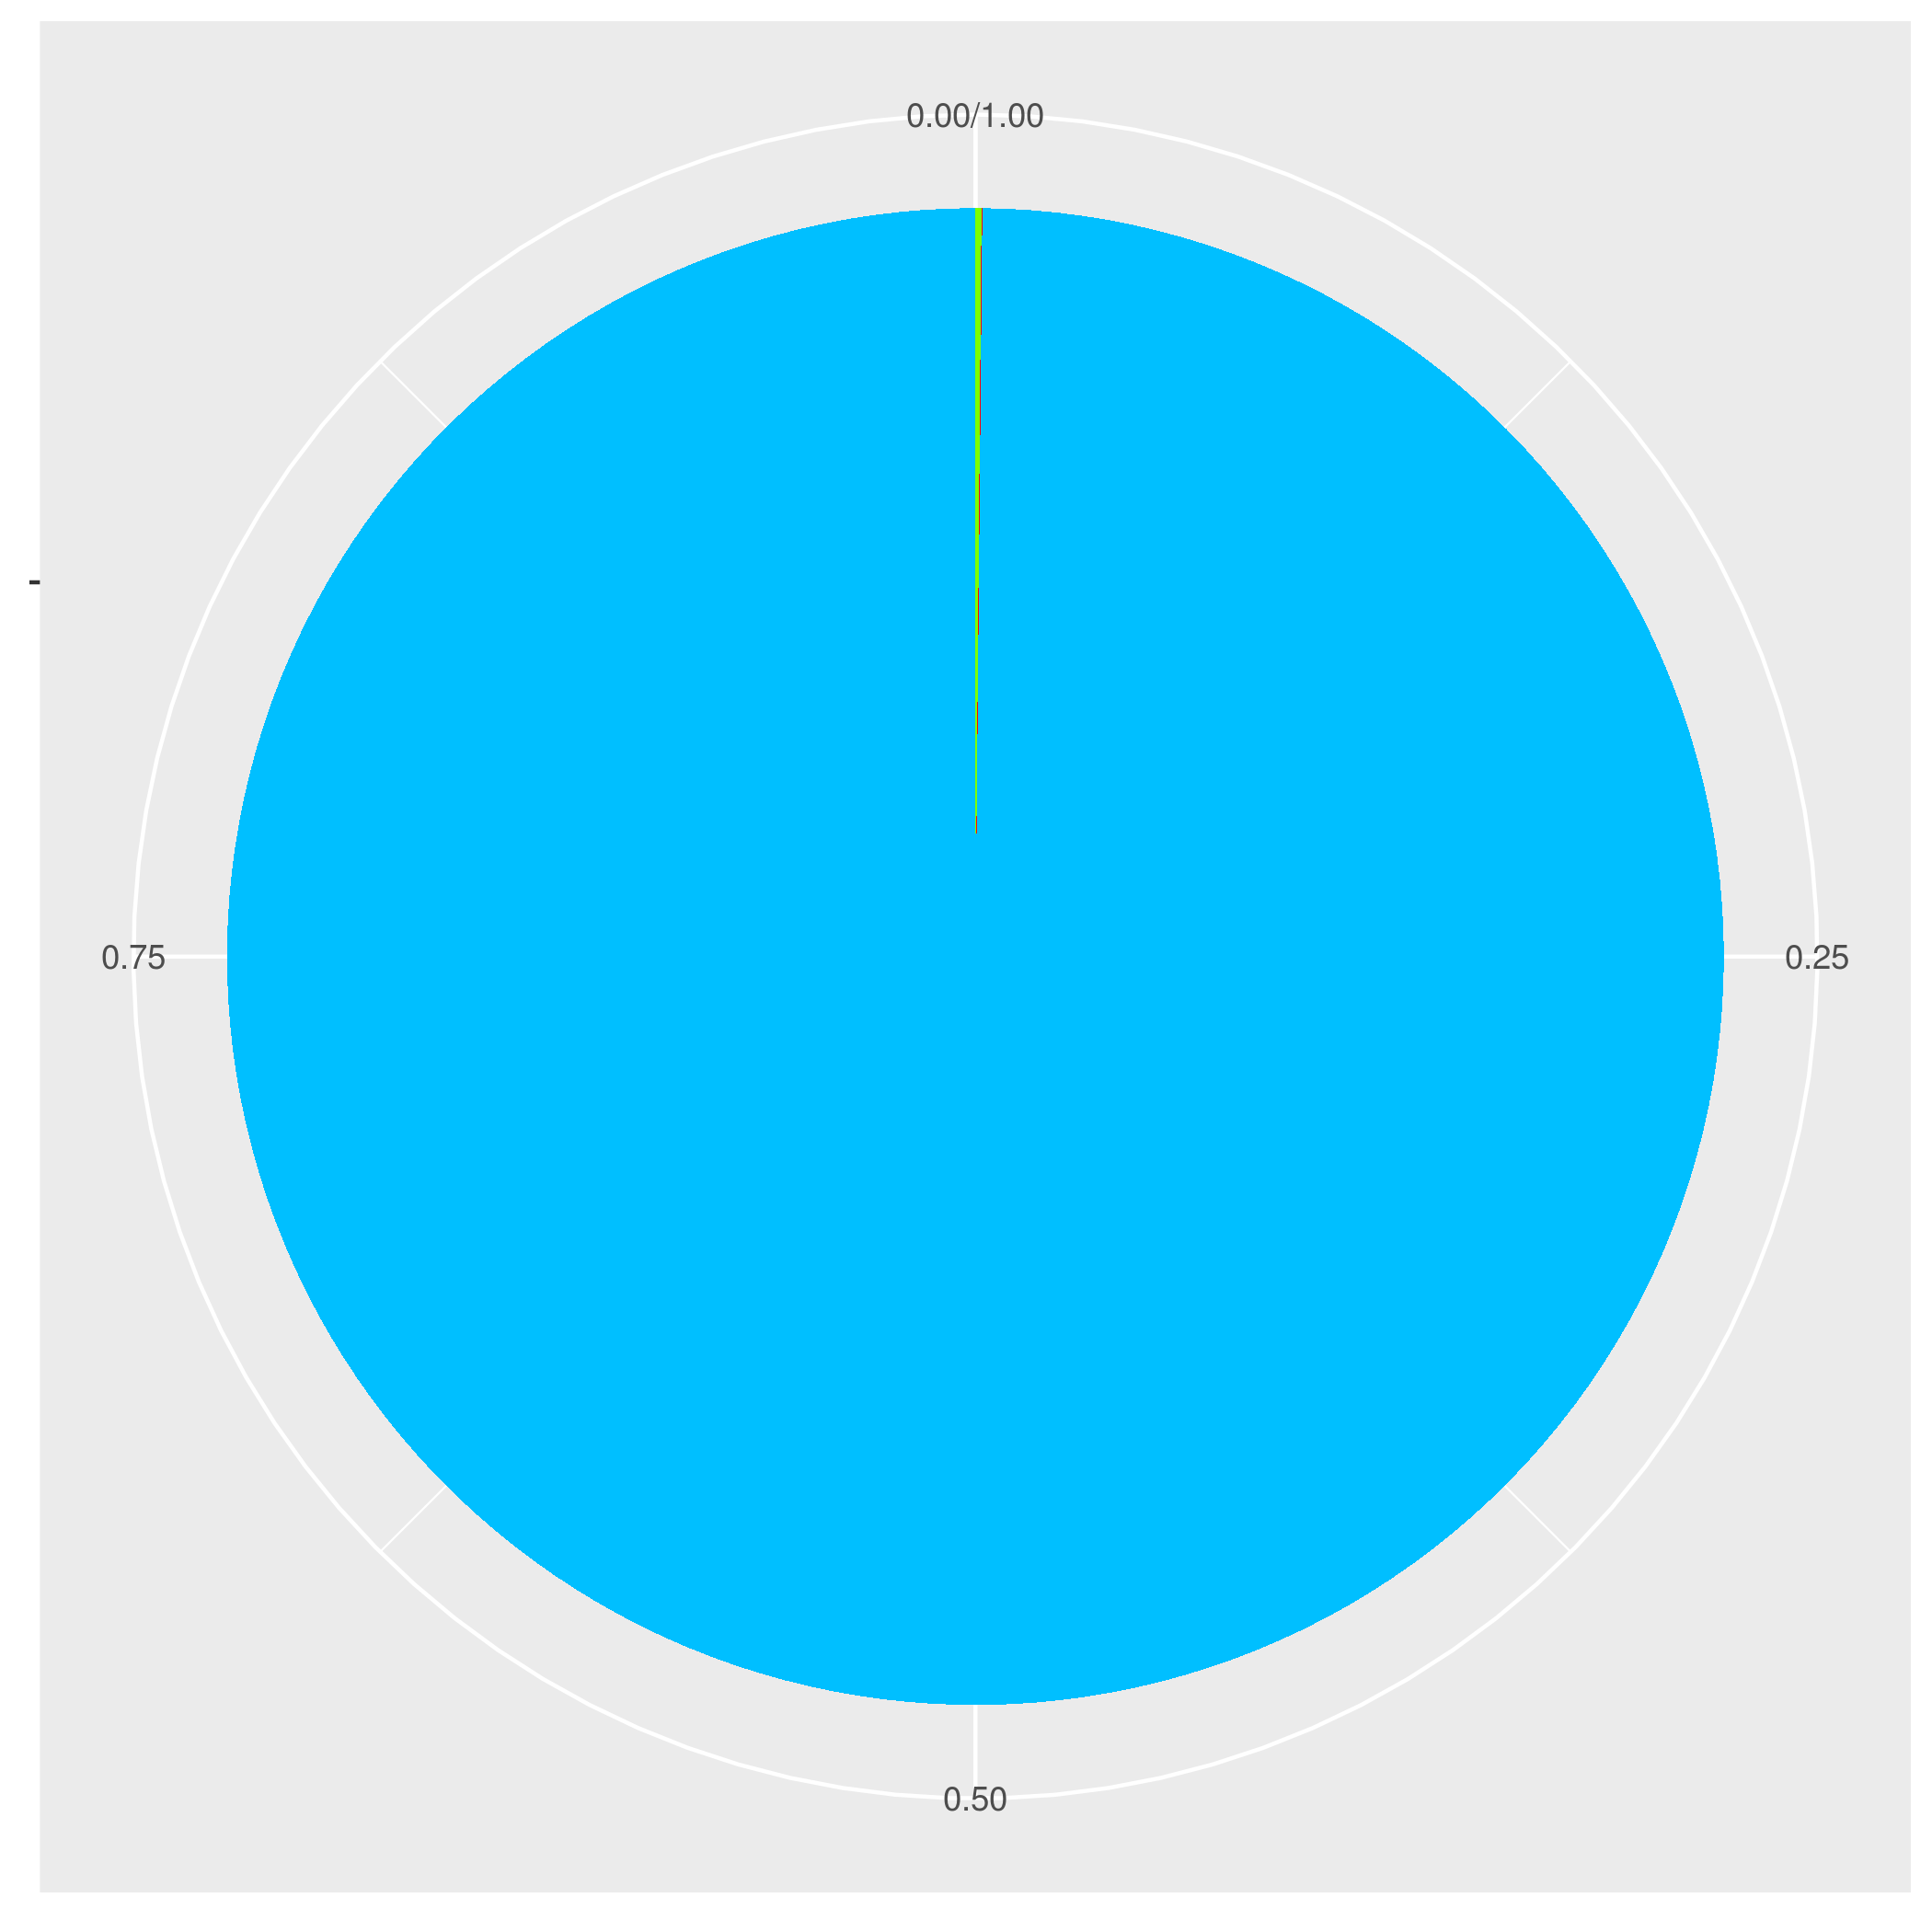
\includegraphics[width=.25\columnwidth]{kosarak.dat/toivonen-c3.png}\\
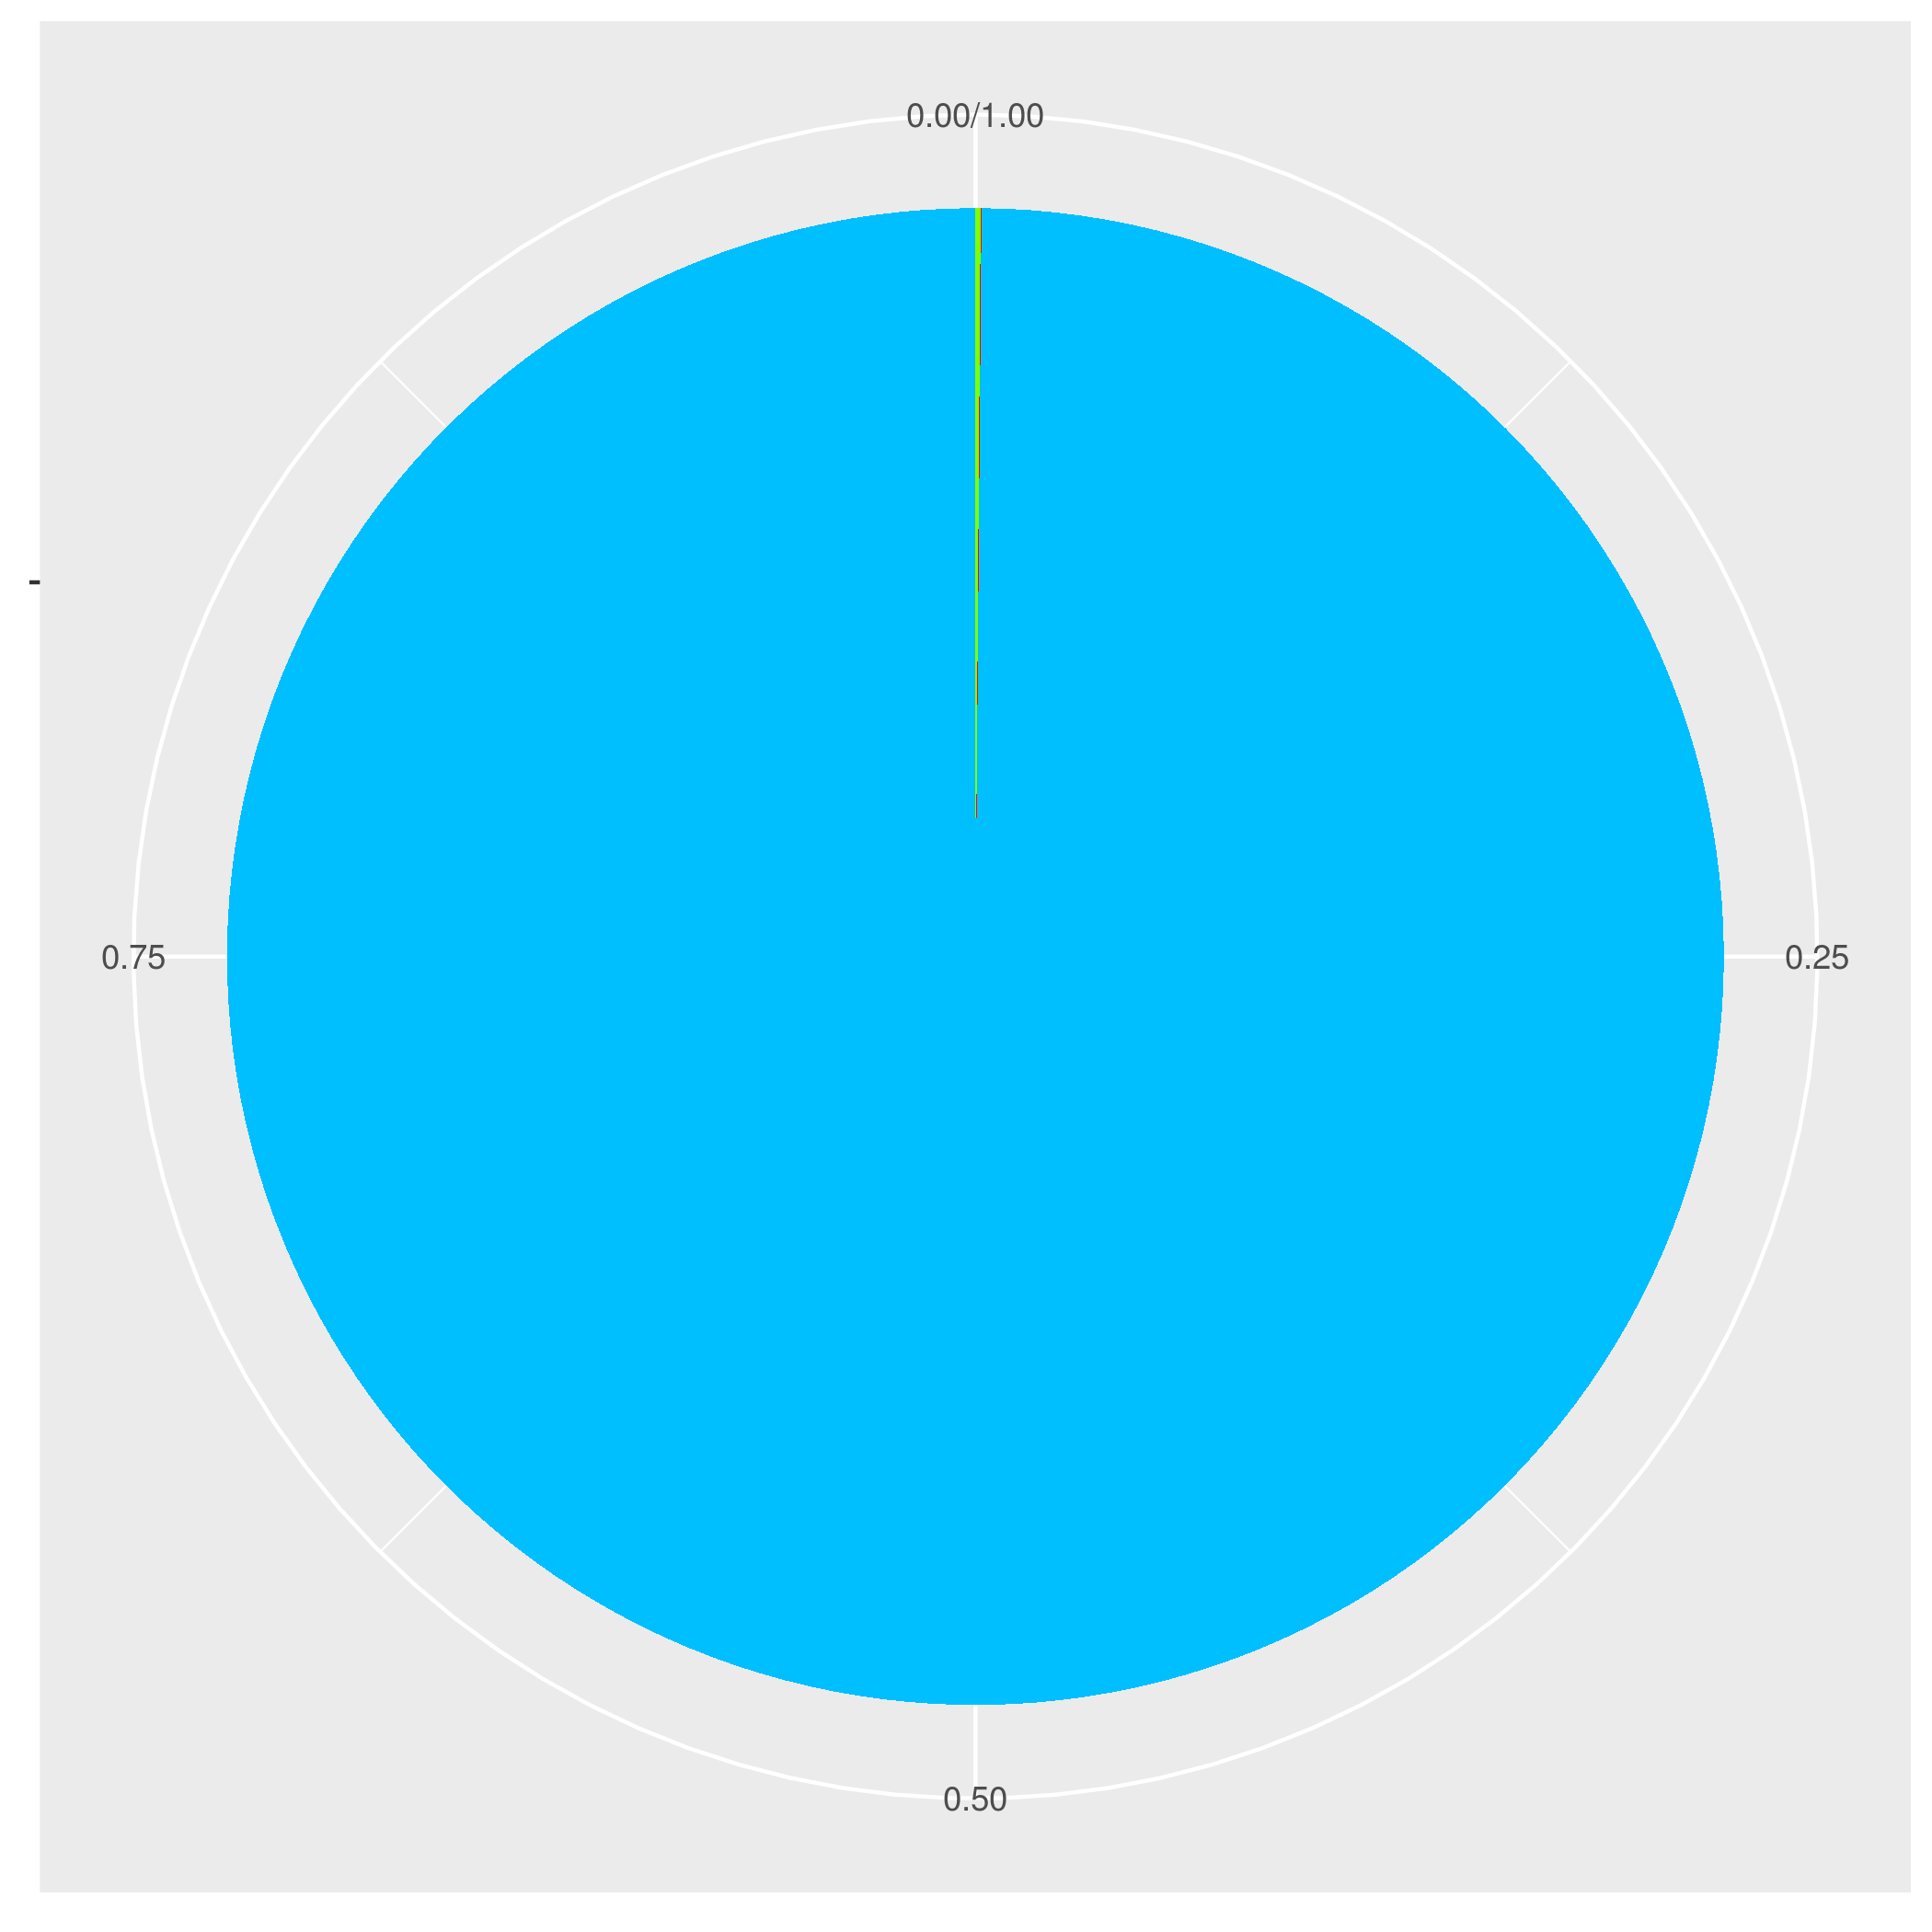
\includegraphics[width=.25\columnwidth]{kosarak.dat/toivonen-c4.png}
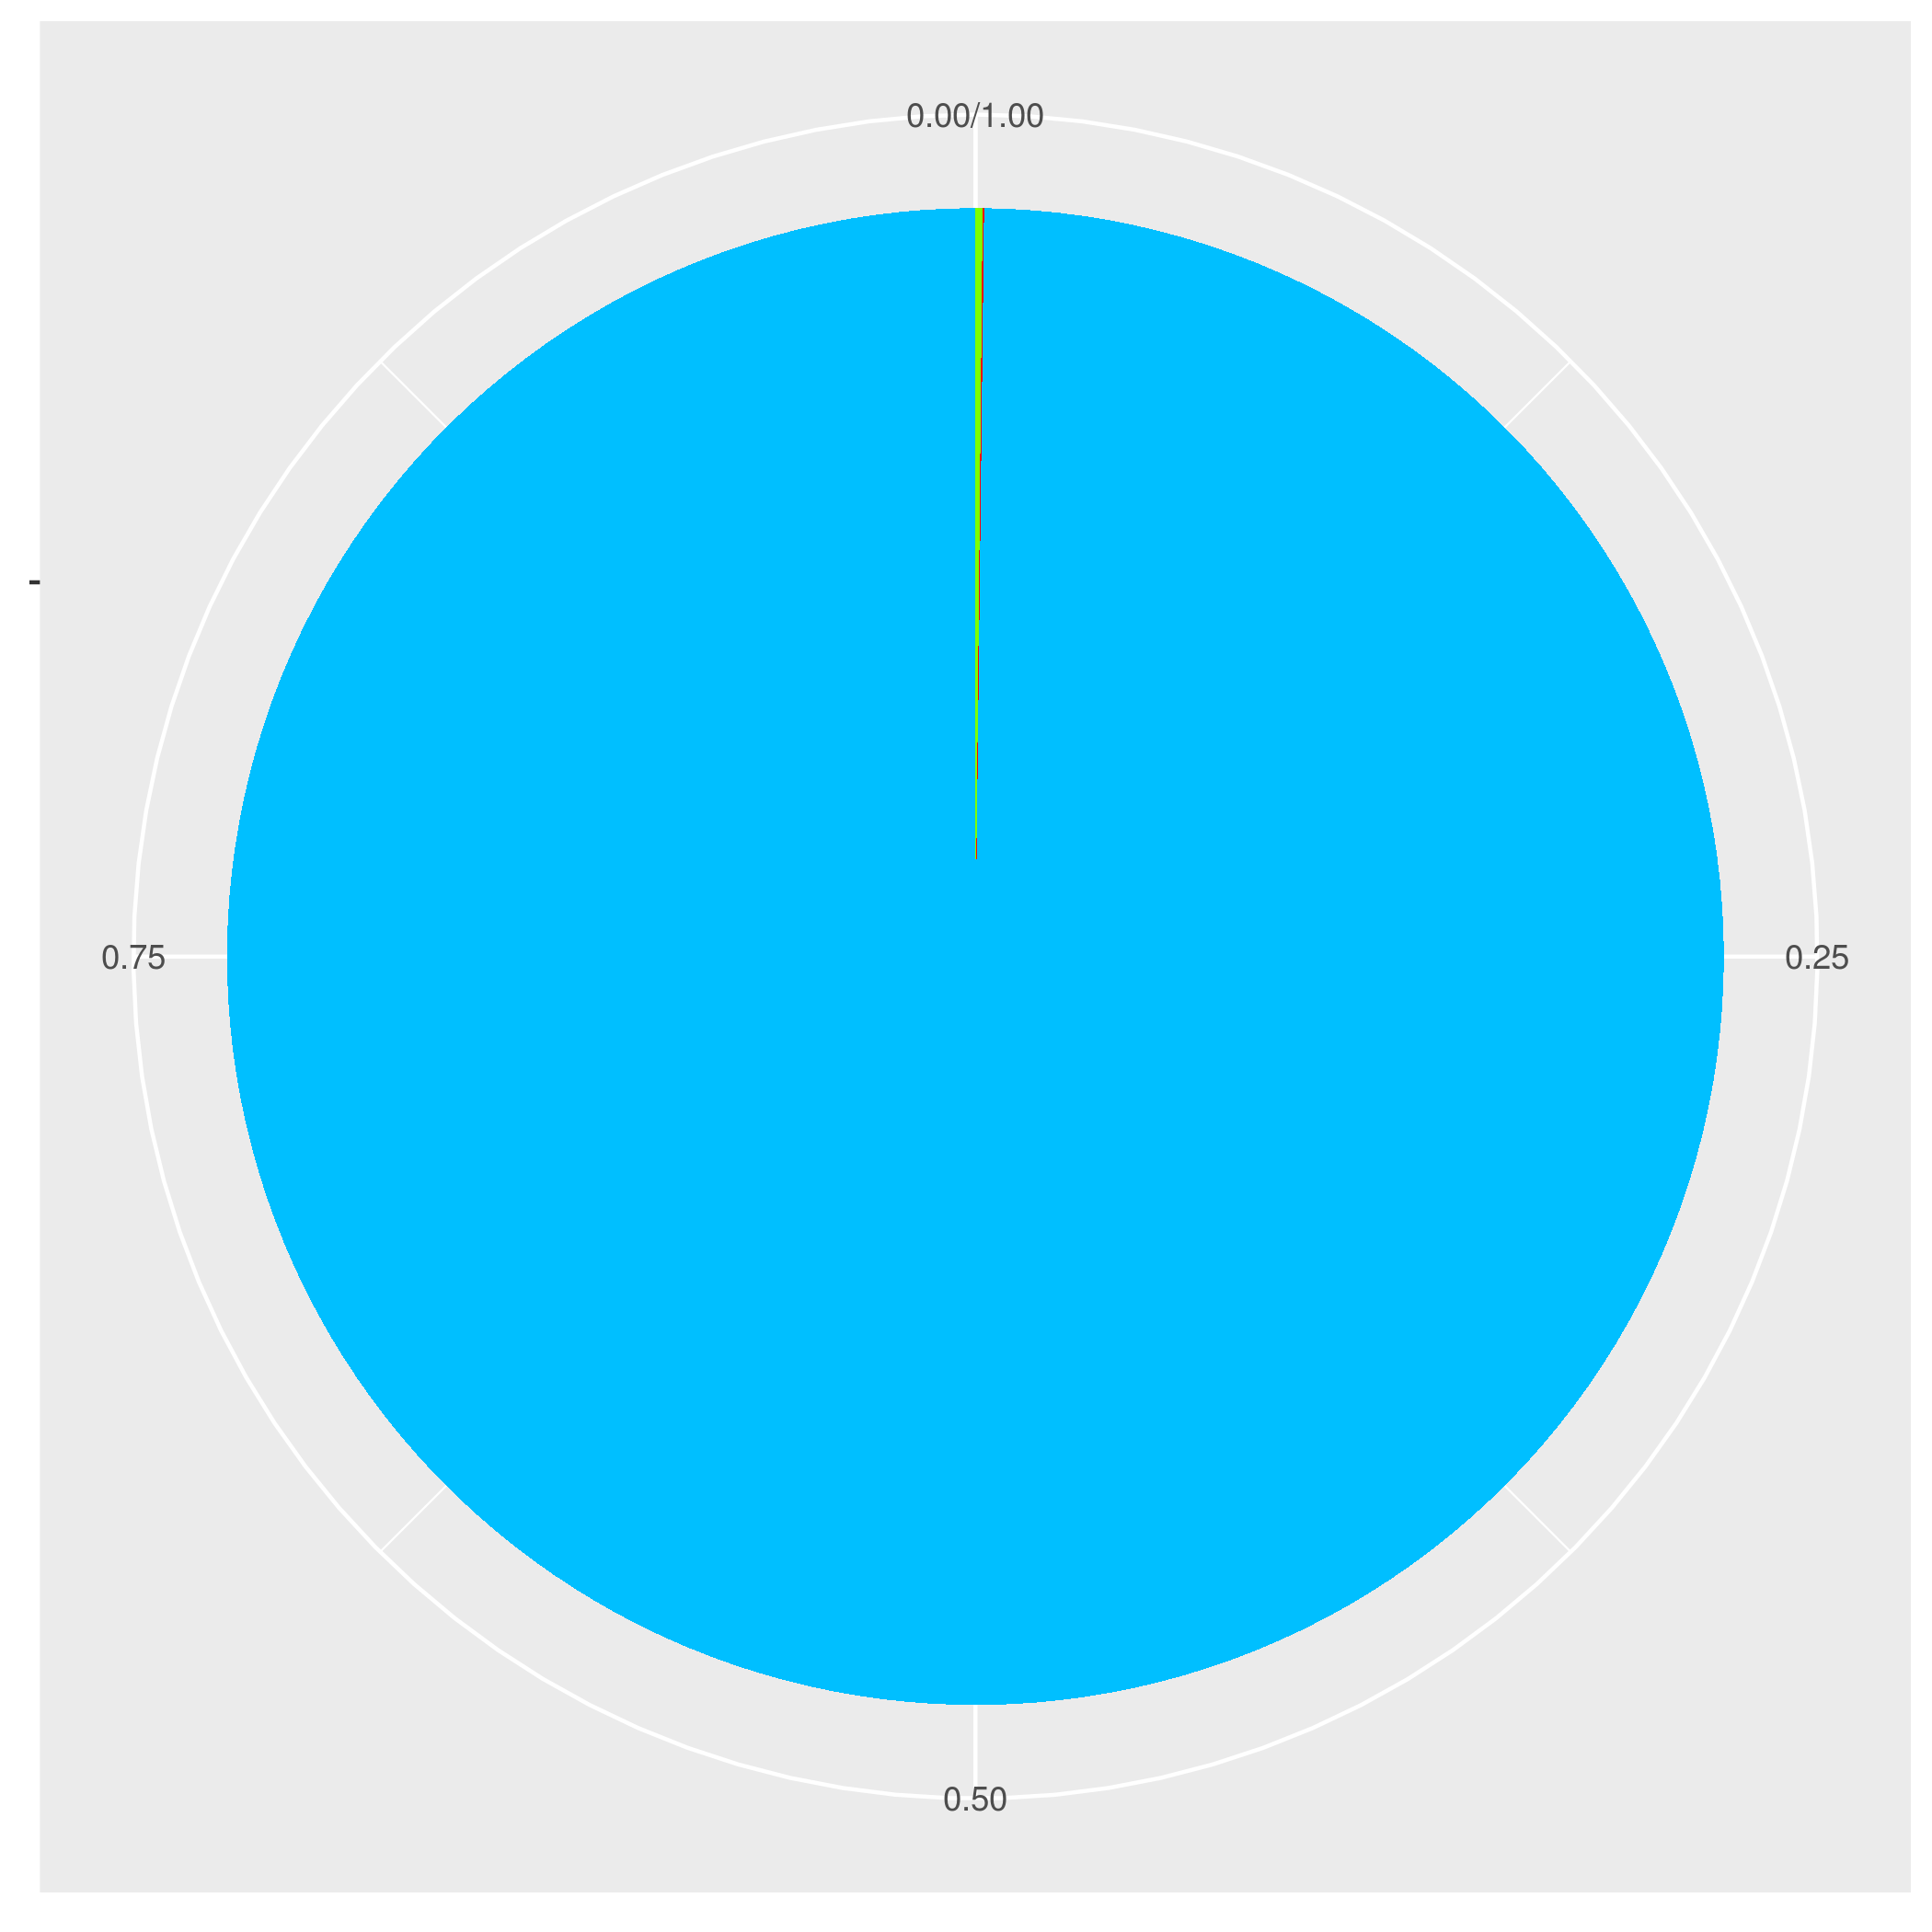
\includegraphics[width=.25\columnwidth]{kosarak.dat/toivonen-c5.png}
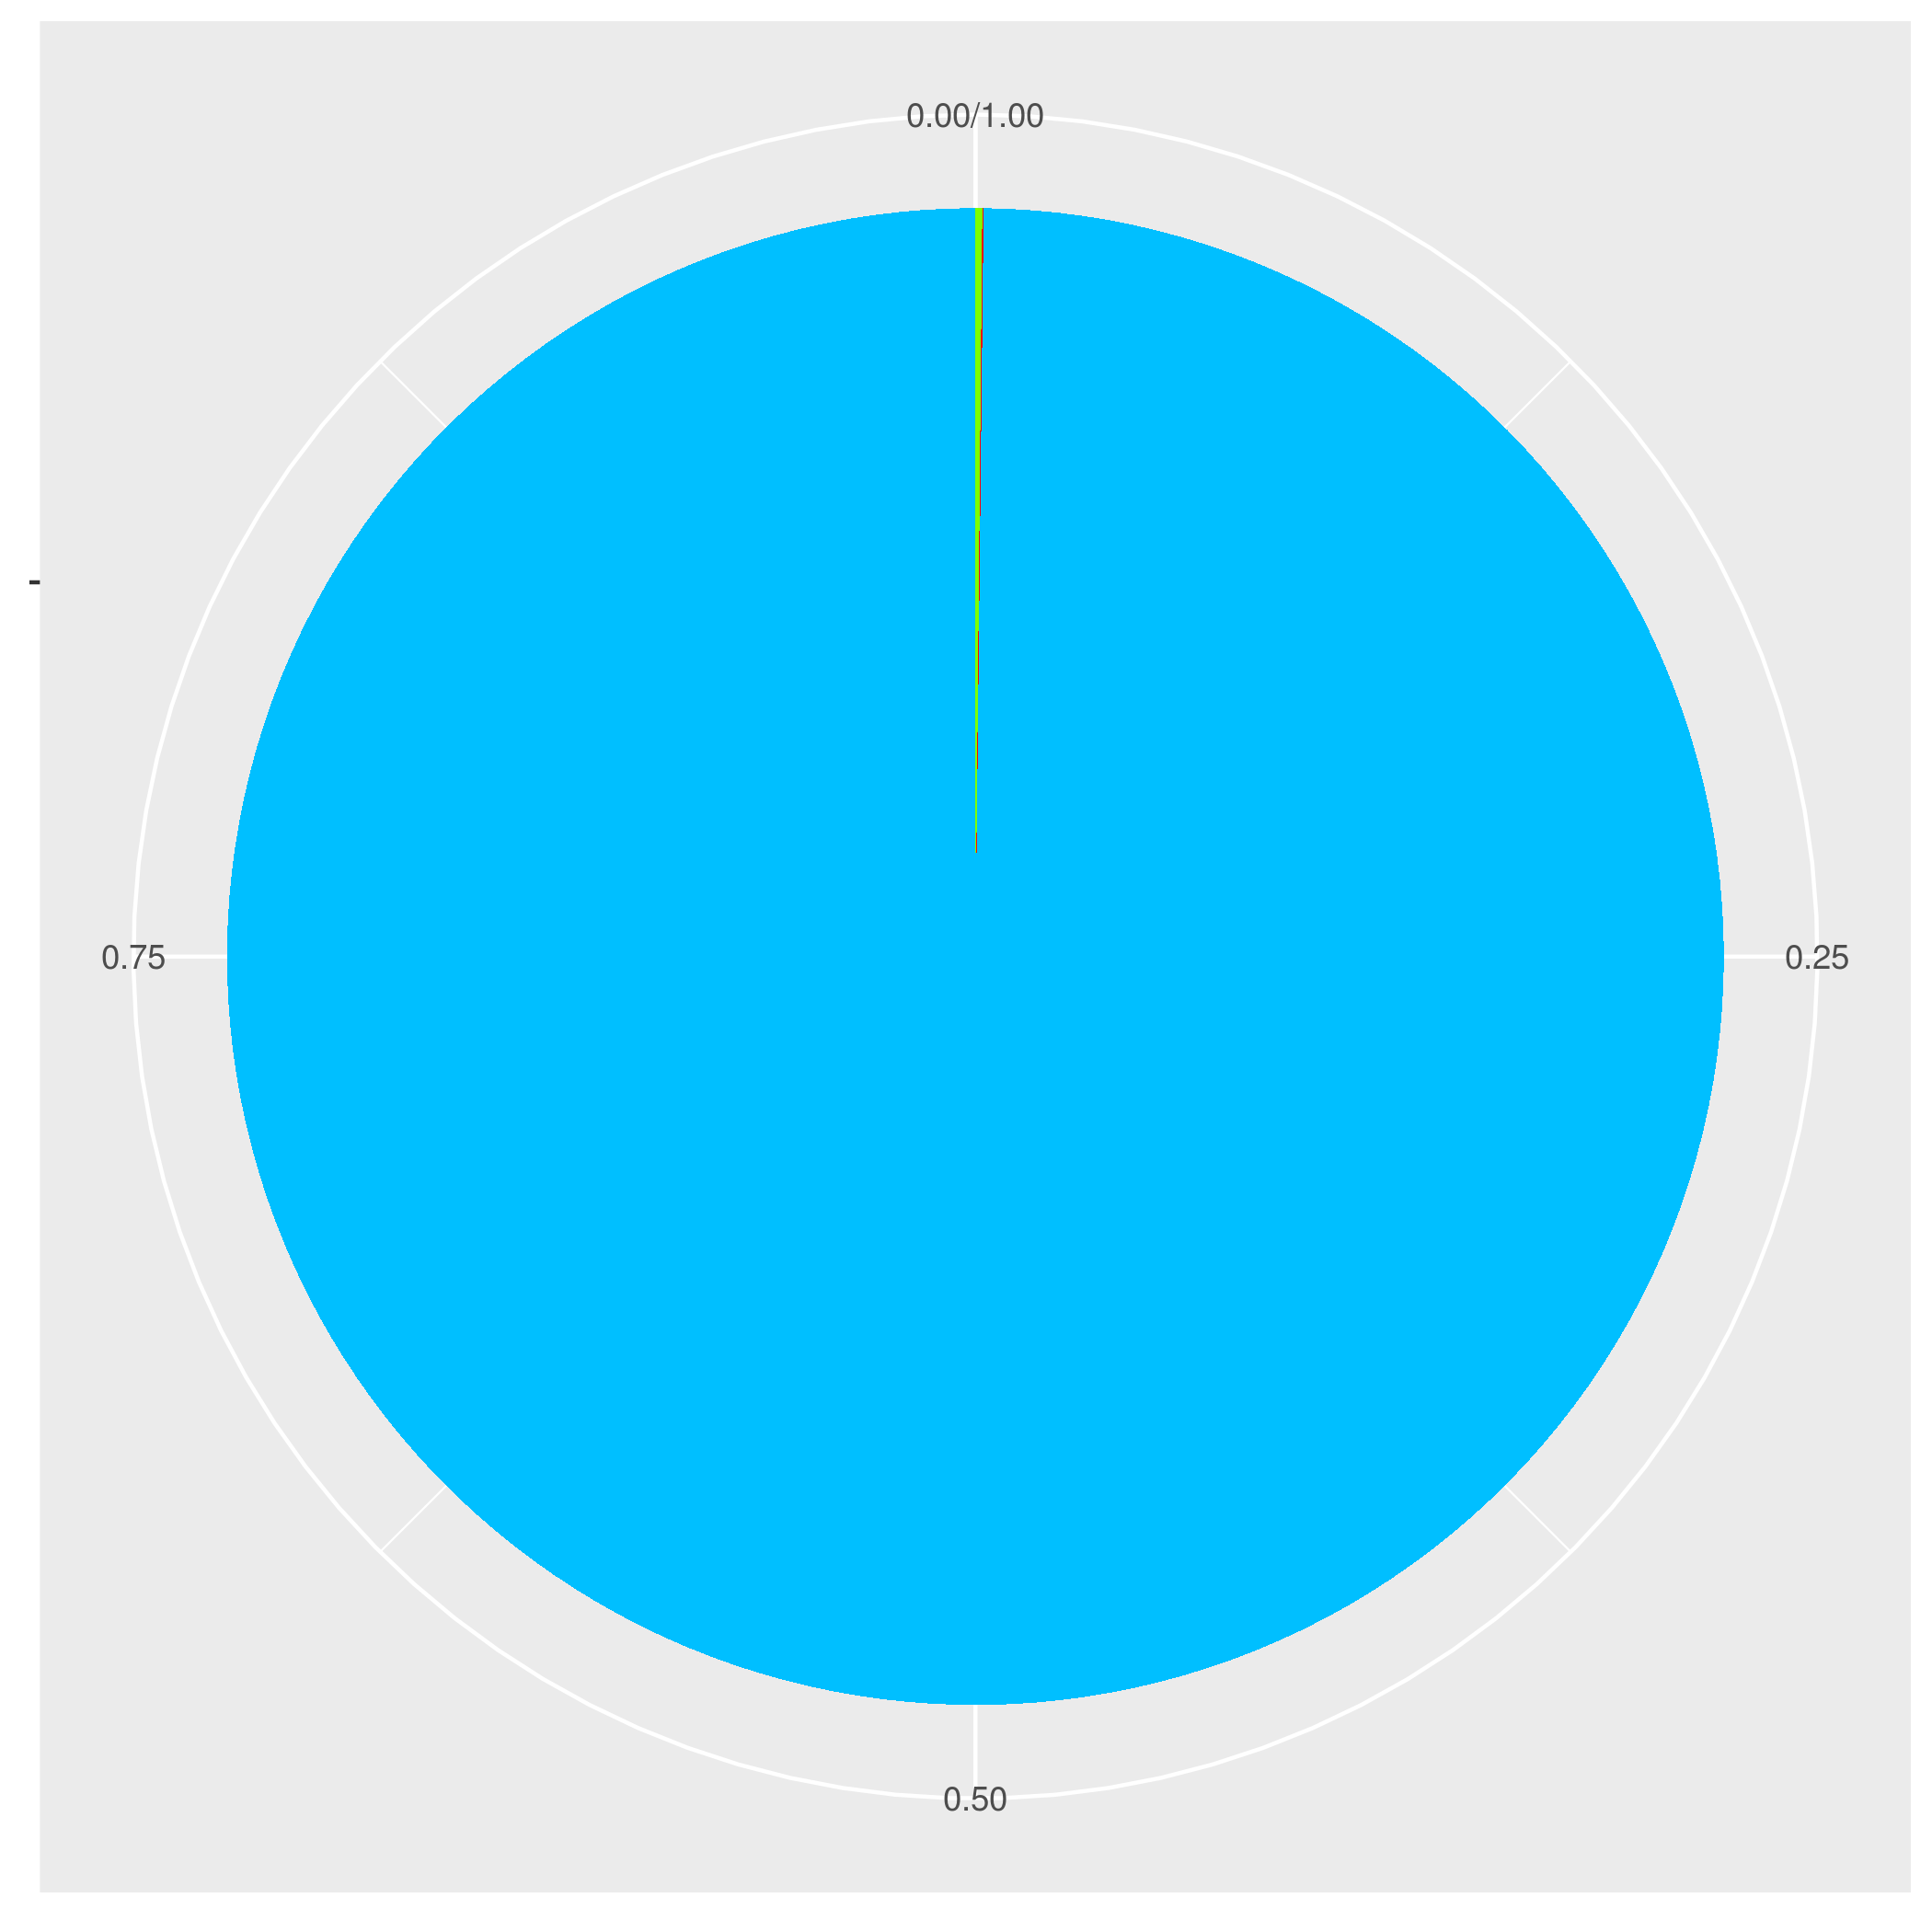
\includegraphics[width=.25\columnwidth]{kosarak.dat/toivonen-c6.png}
\end{figure}
\vspace{-.45cm}
\begin{figure}[h!]
\centering
\caption*{Riondato}
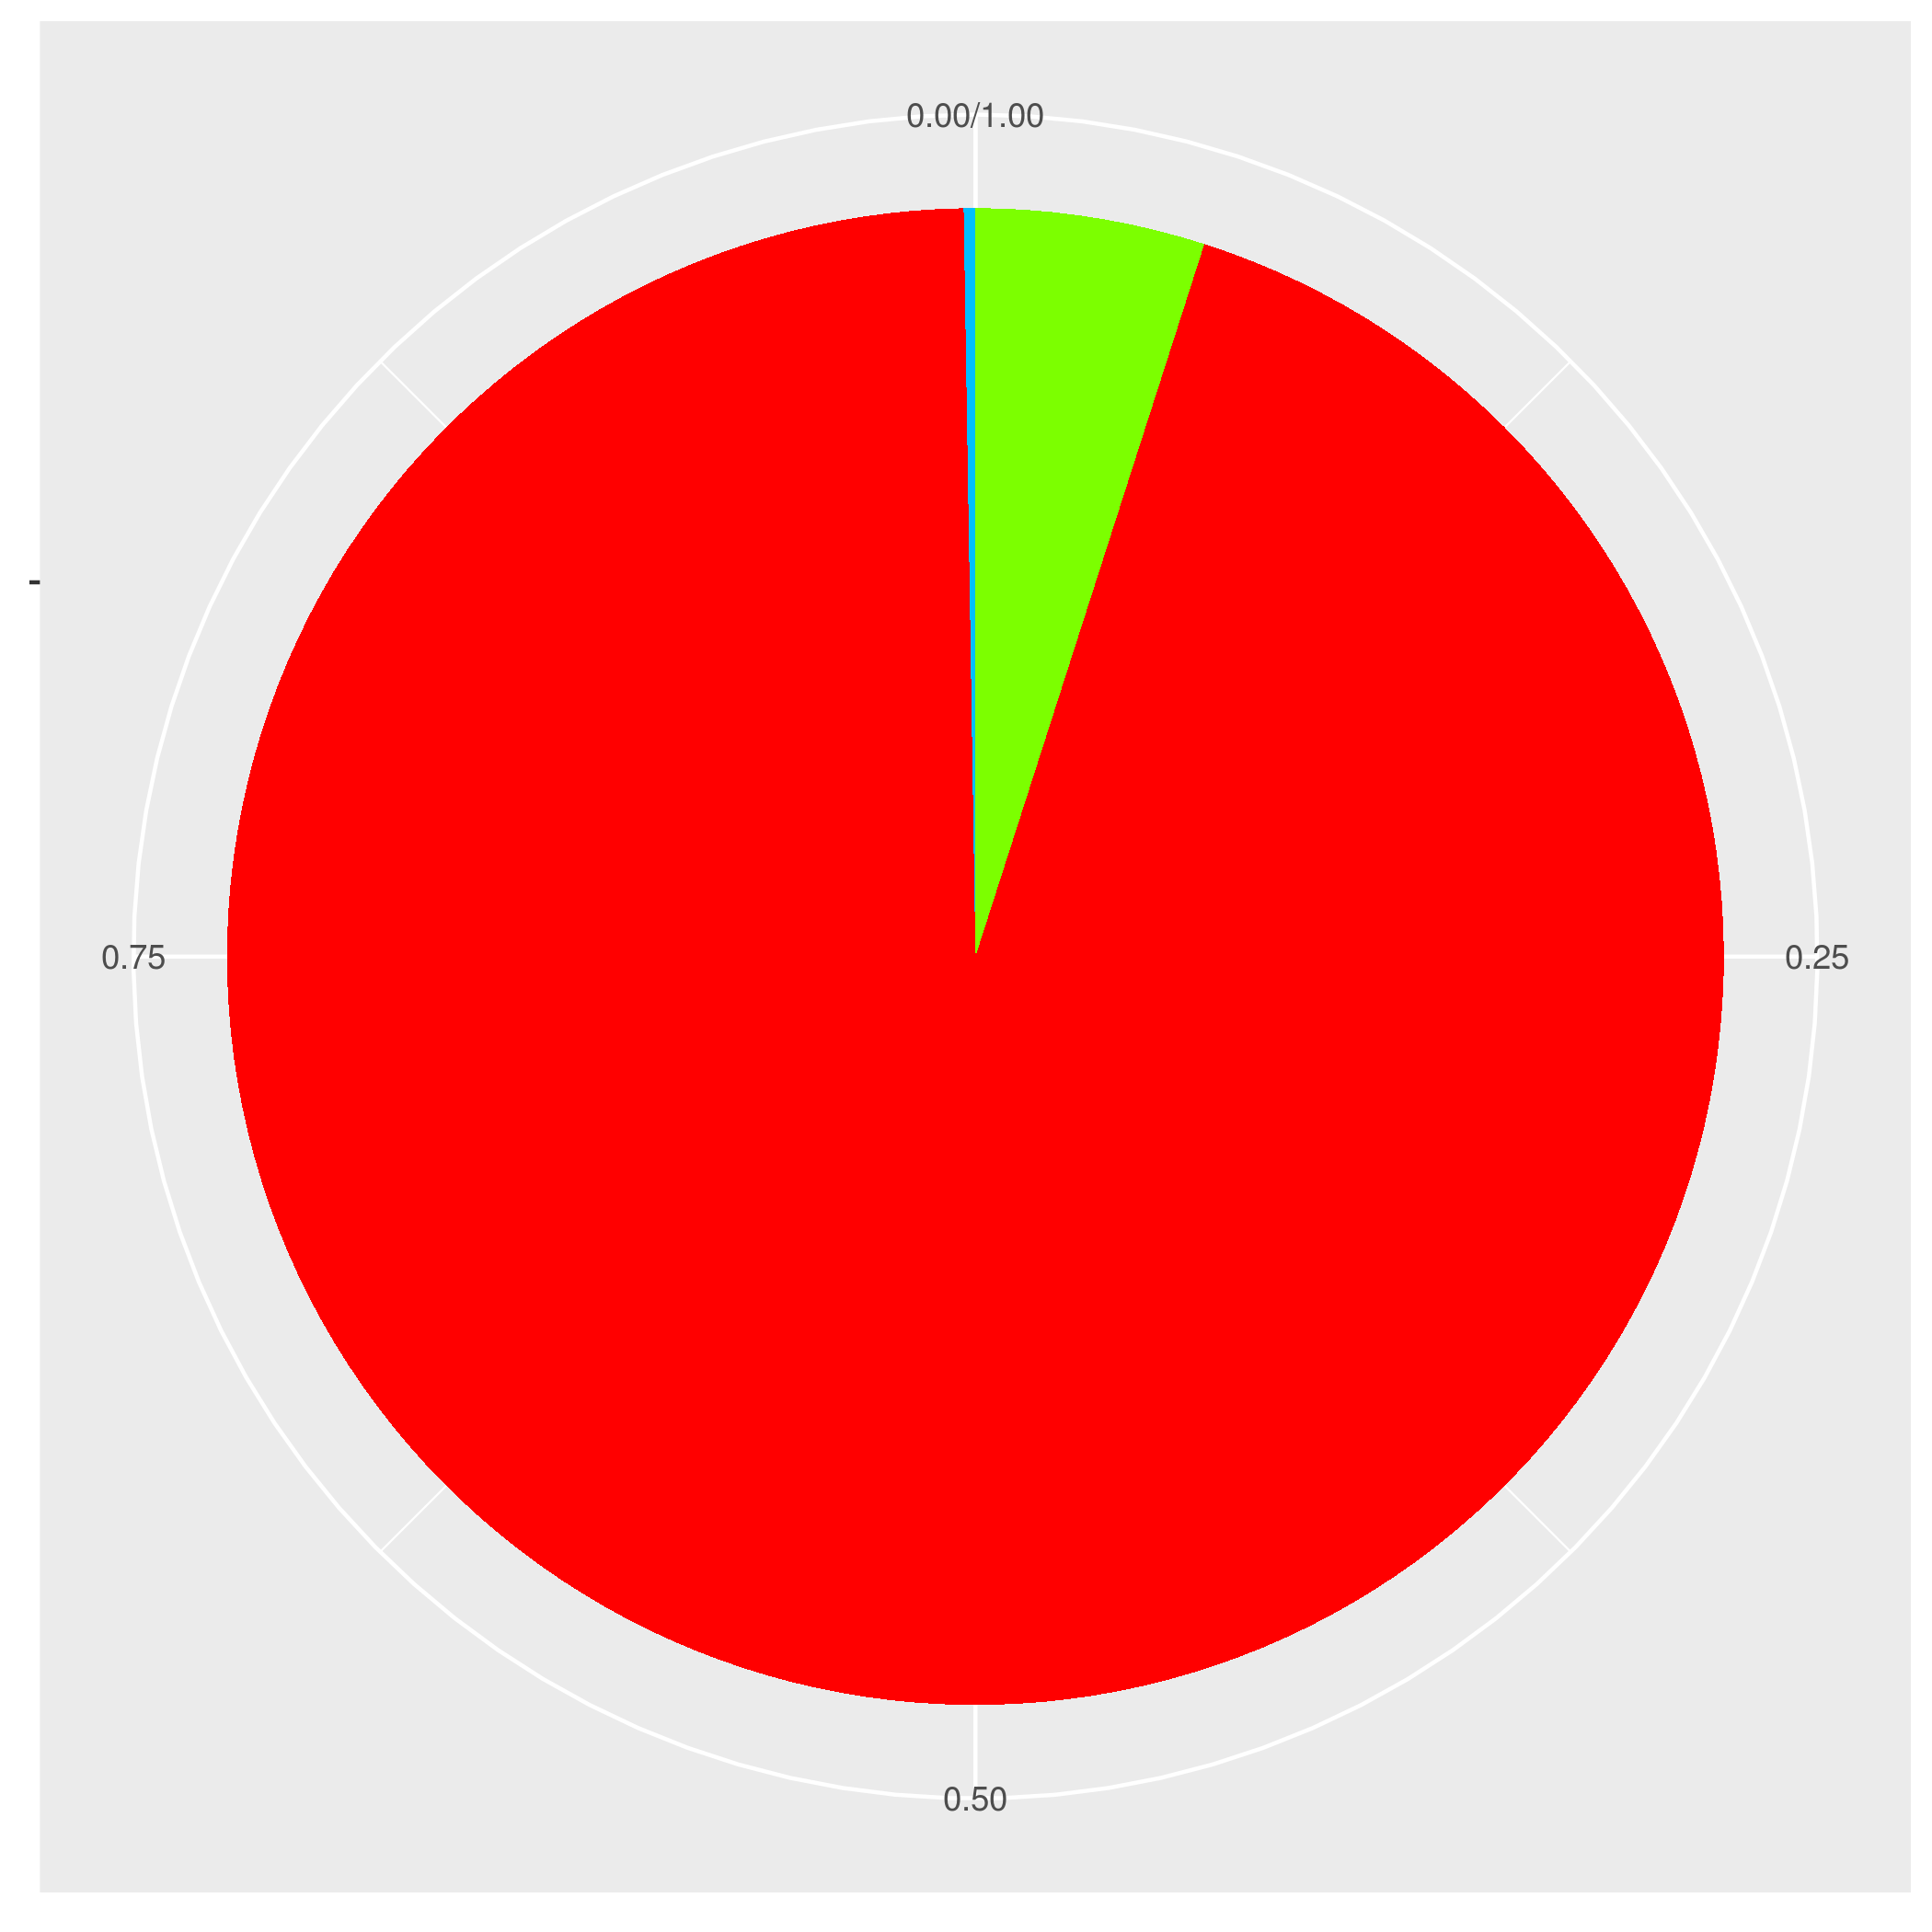
\includegraphics[width=.25\columnwidth]{kosarak.dat/riondato-c1.png}
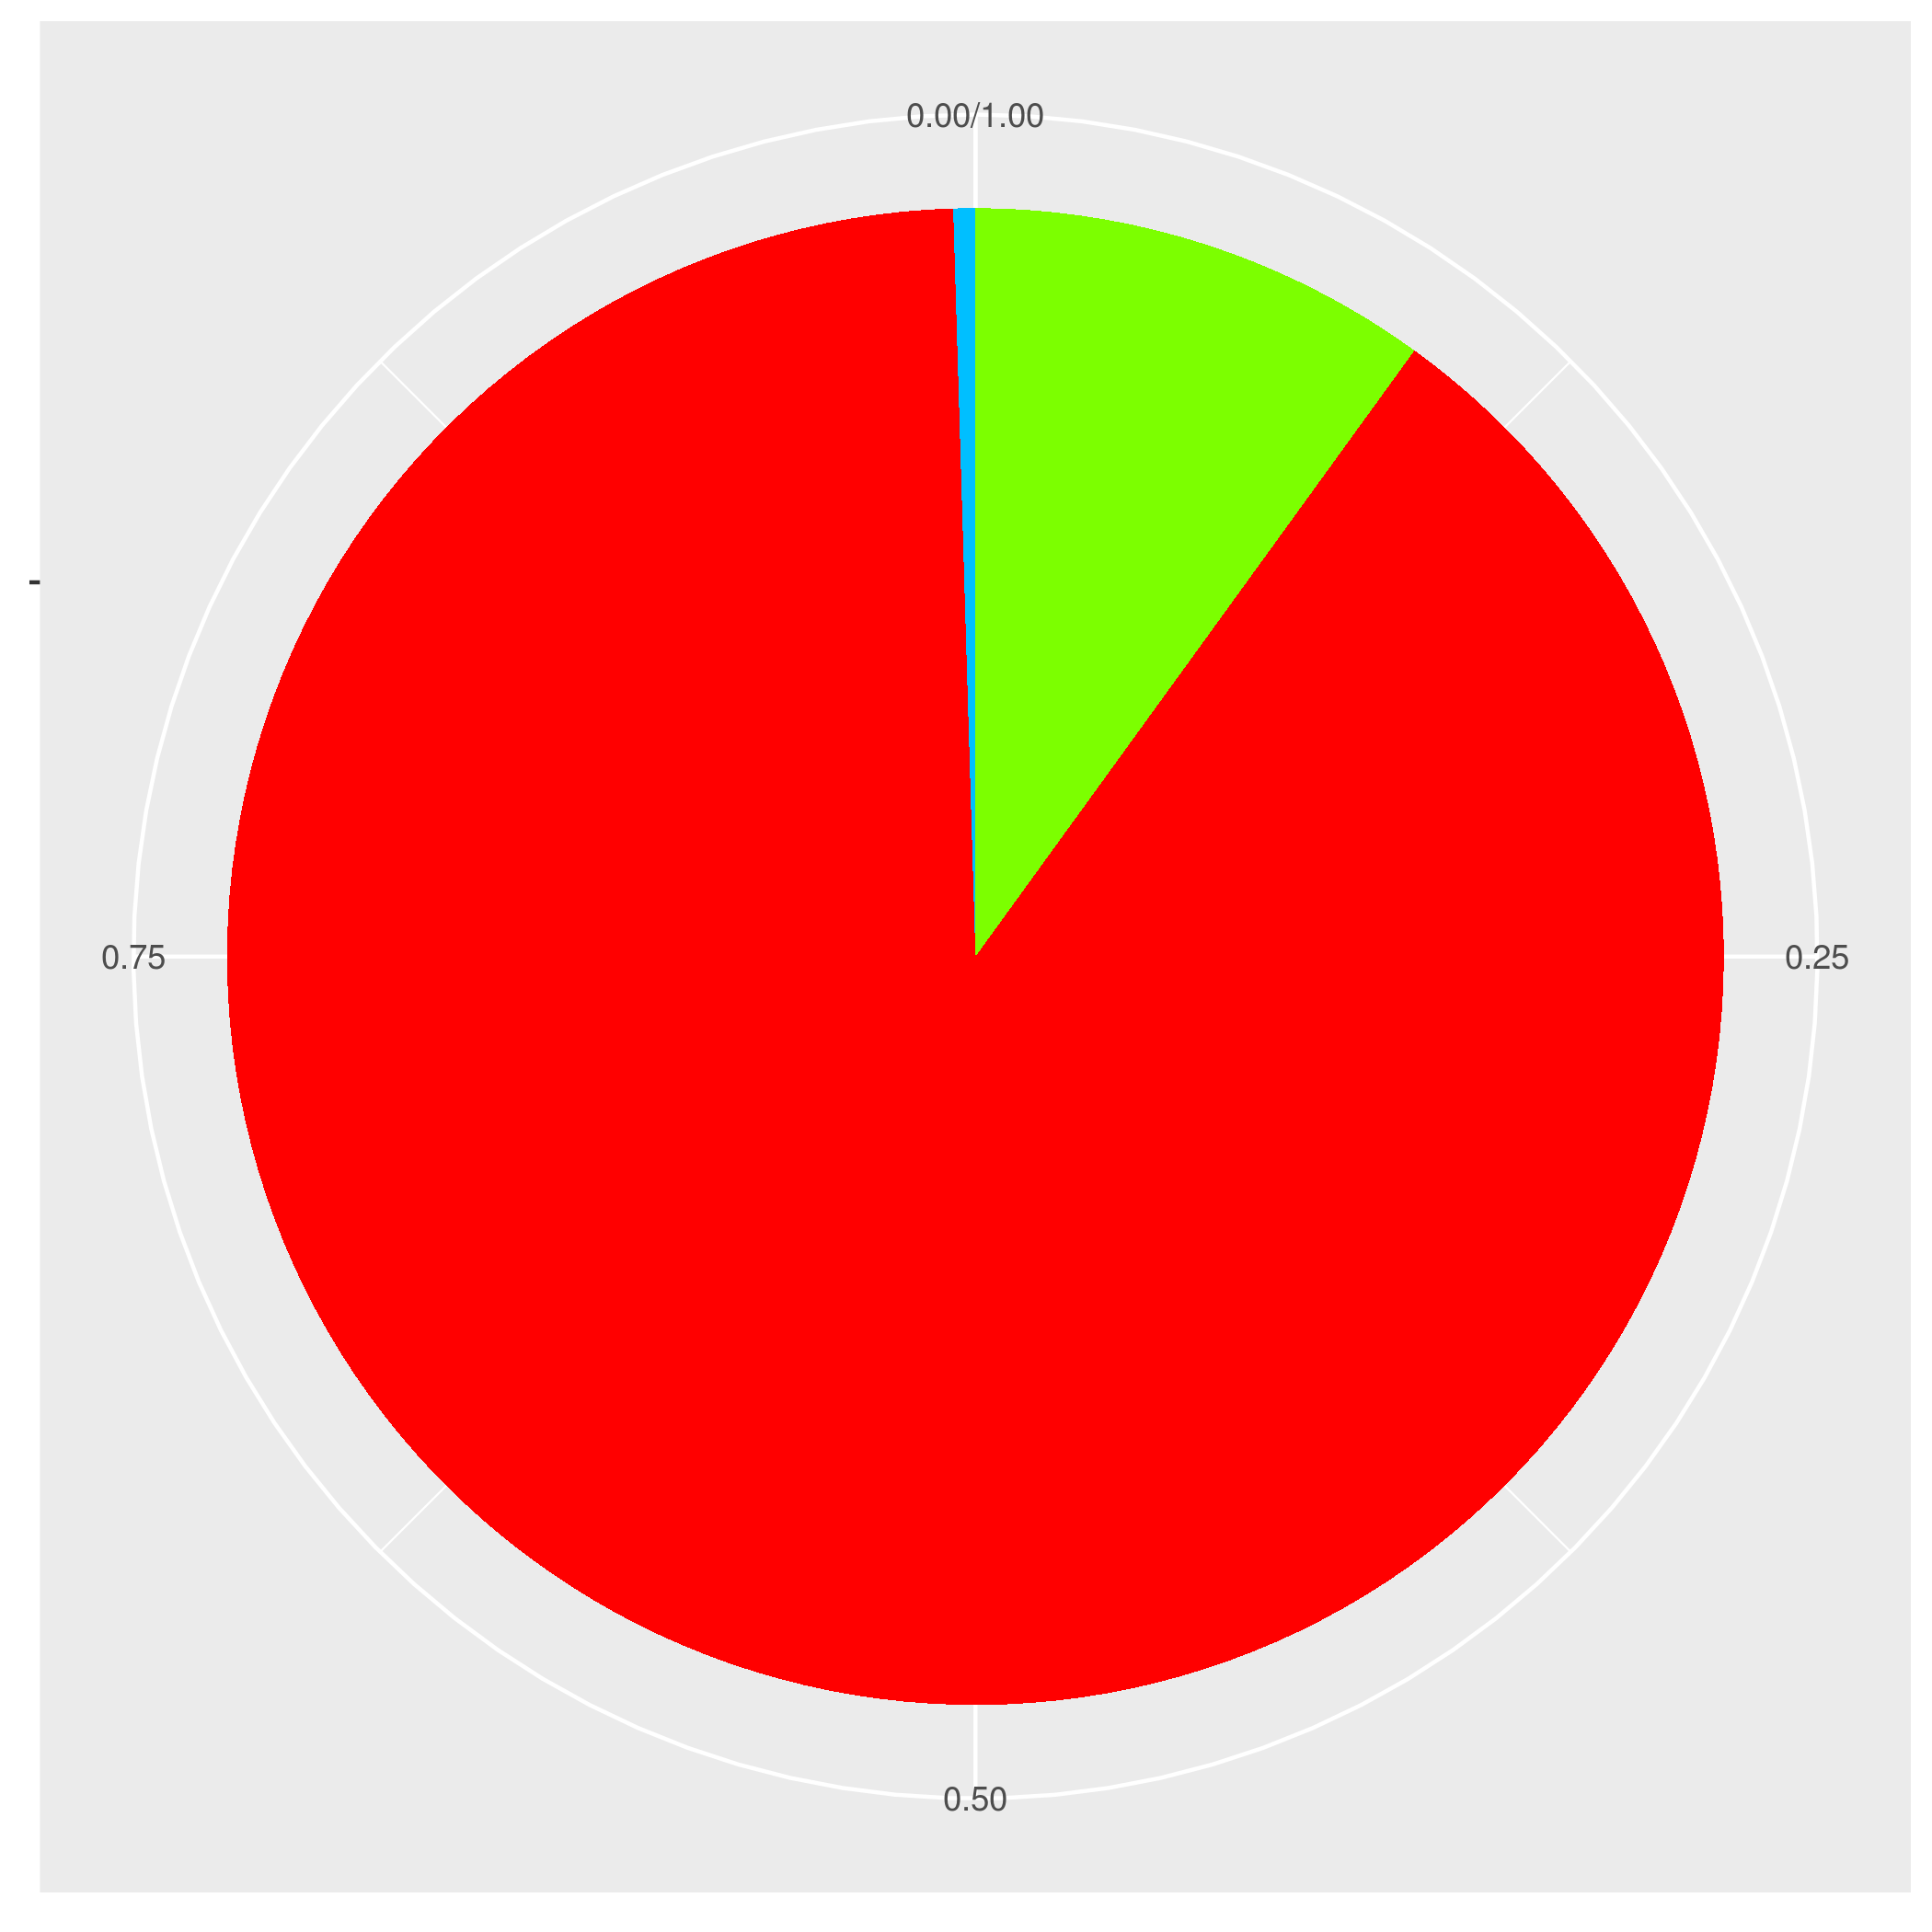
\includegraphics[width=.25\columnwidth]{kosarak.dat/riondato-c2.png}
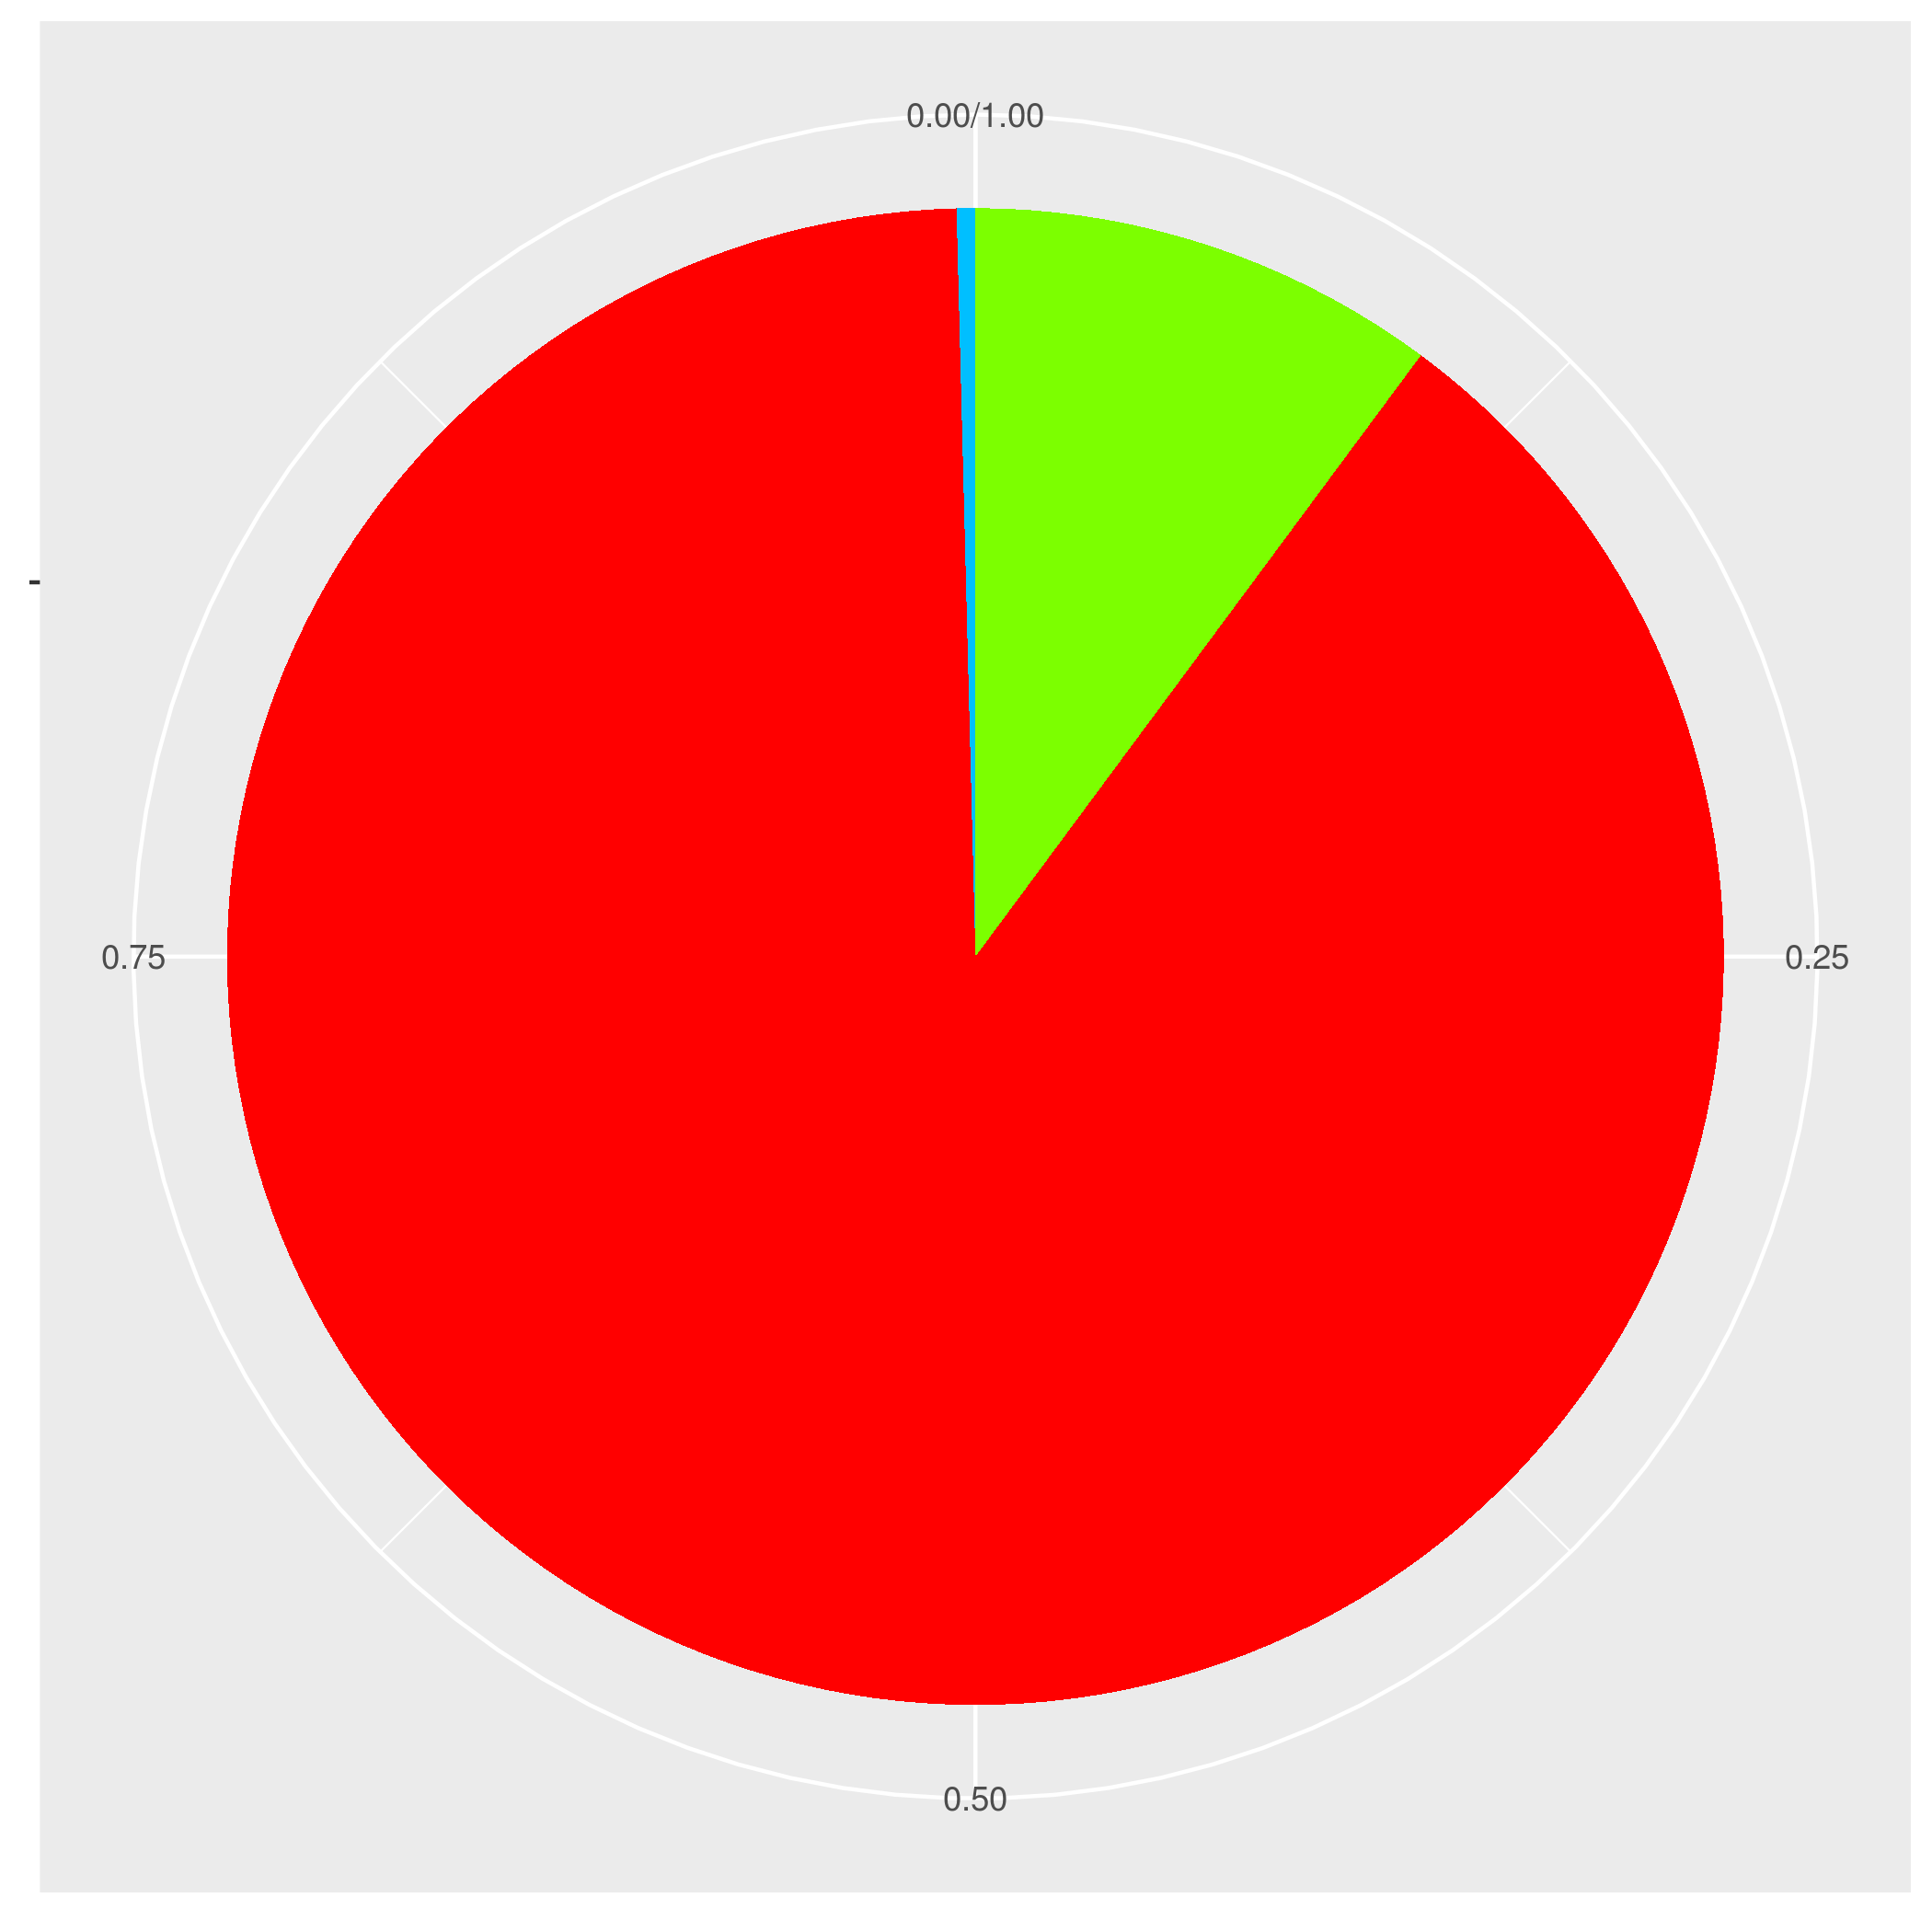
\includegraphics[width=.25\columnwidth]{kosarak.dat/riondato-c3.png}\\
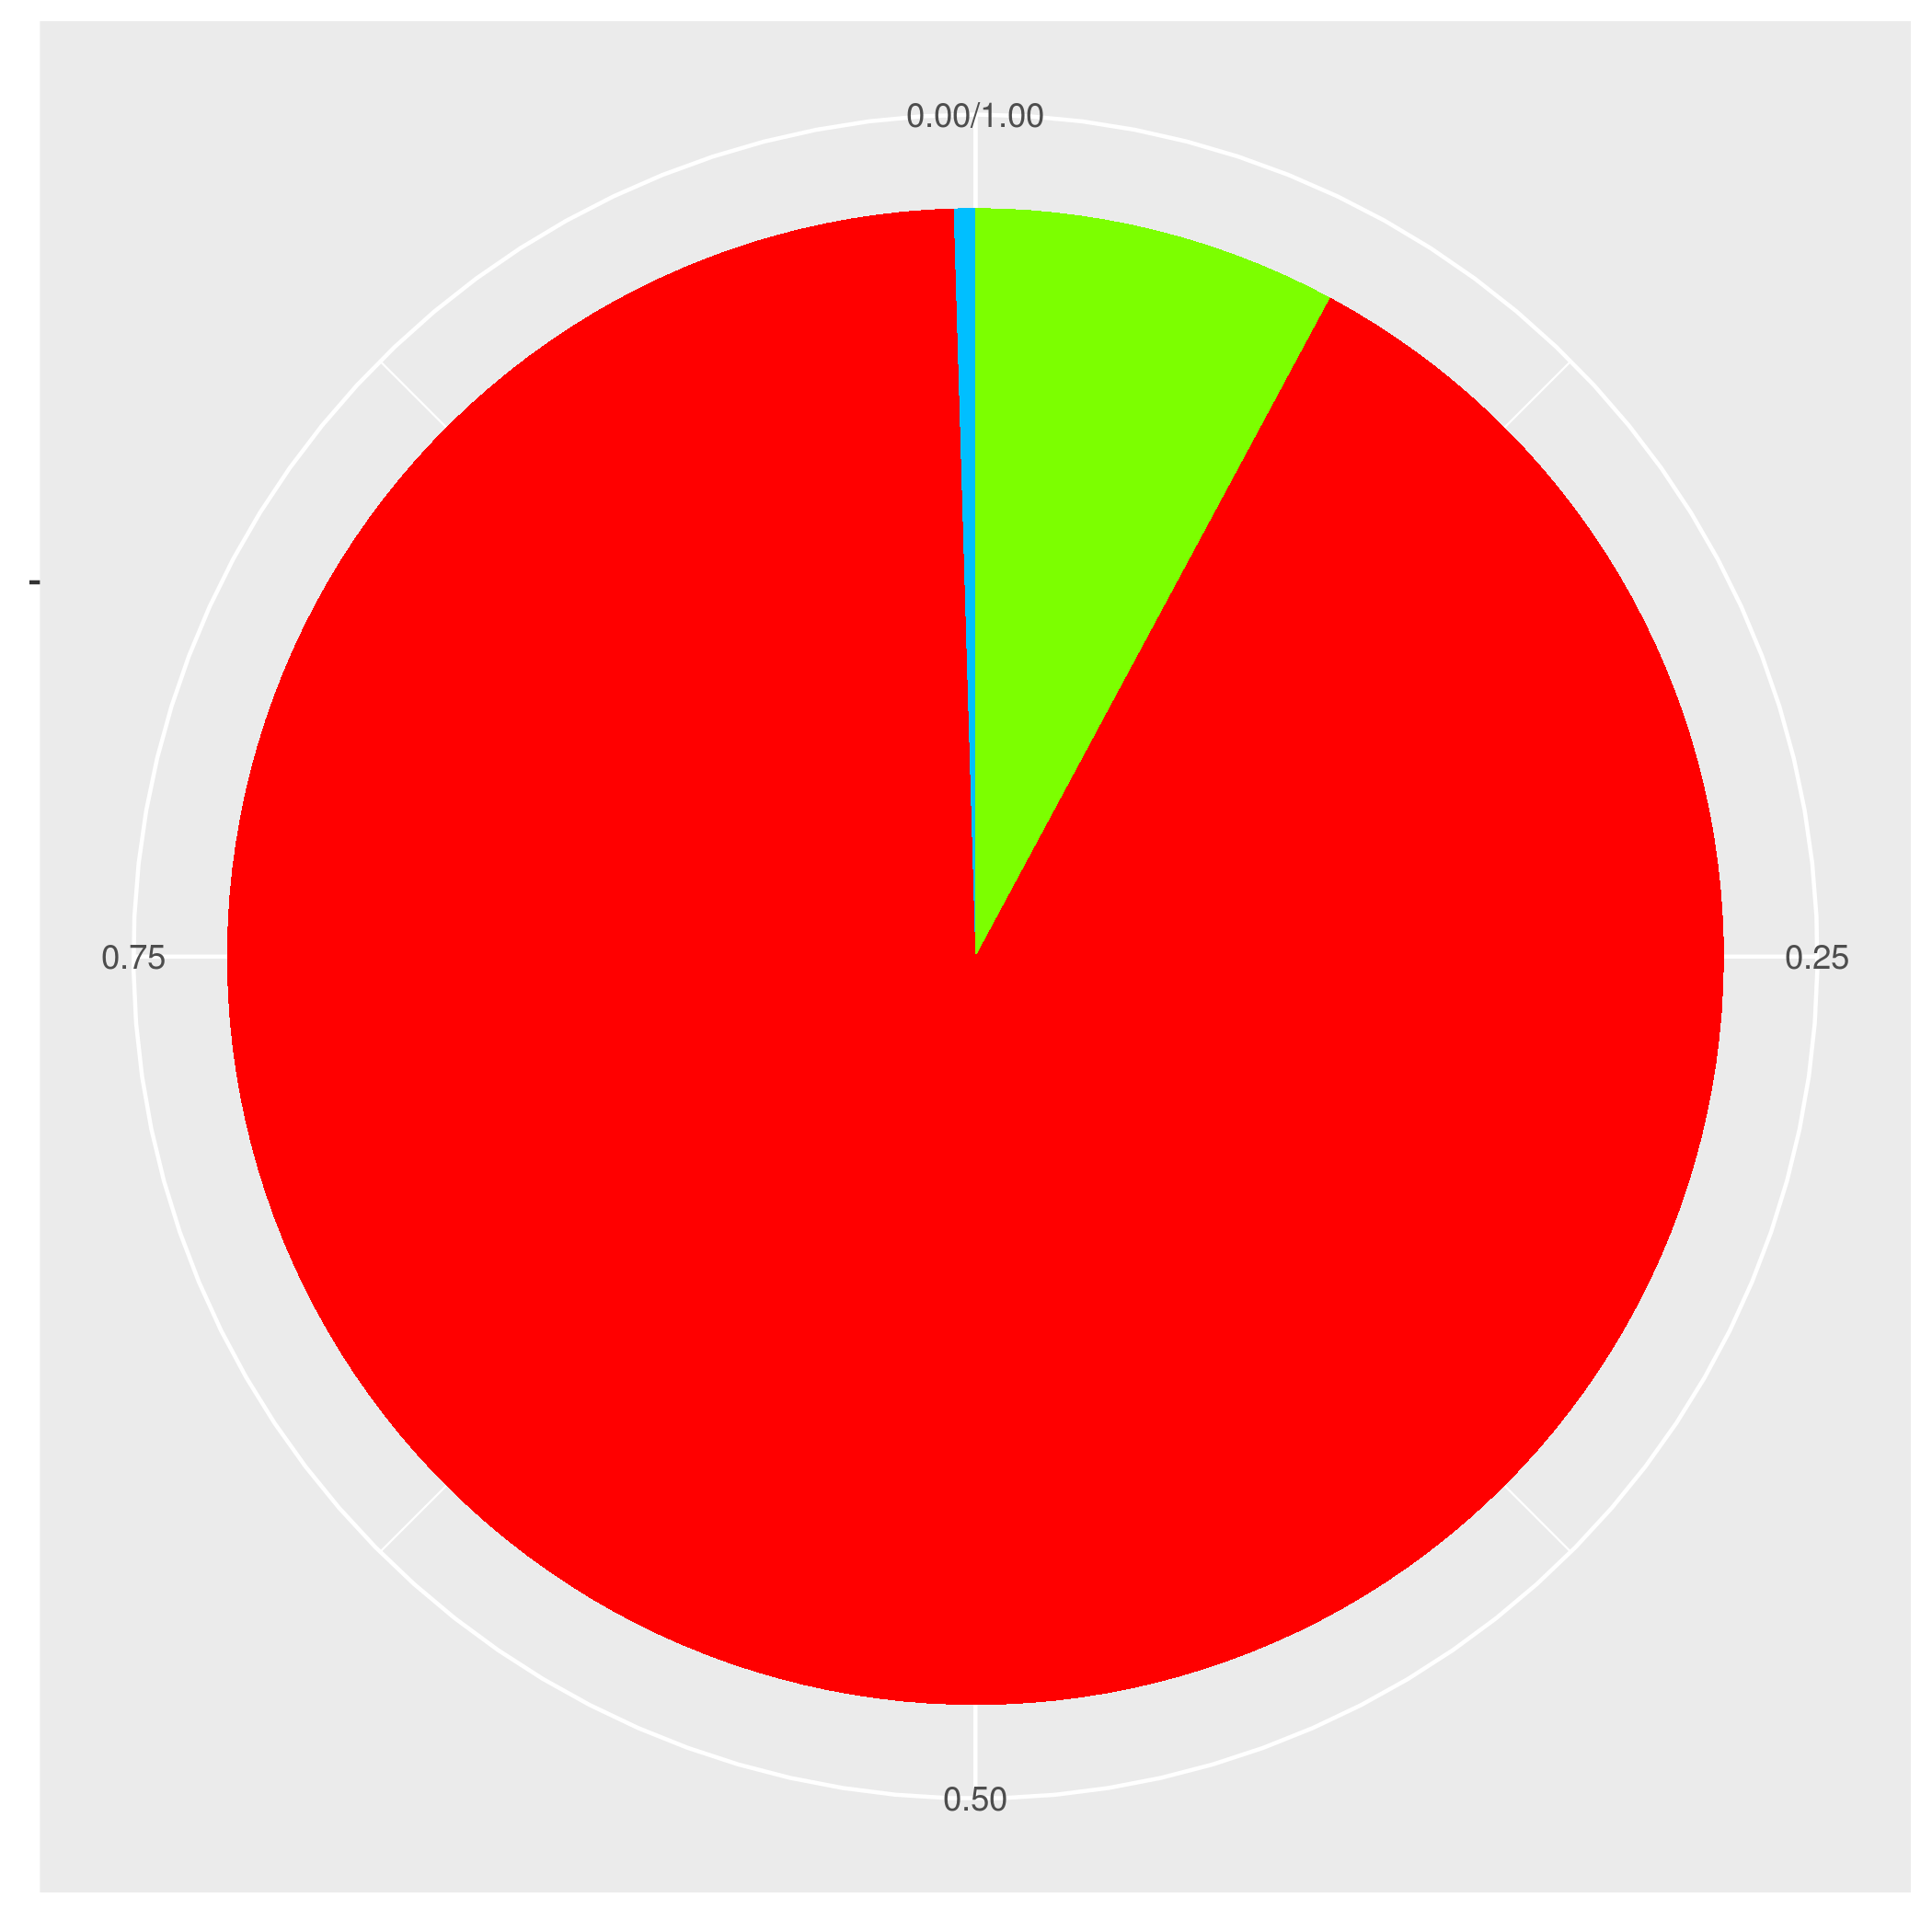
\includegraphics[width=.25\columnwidth]{kosarak.dat/riondato-c4.png}
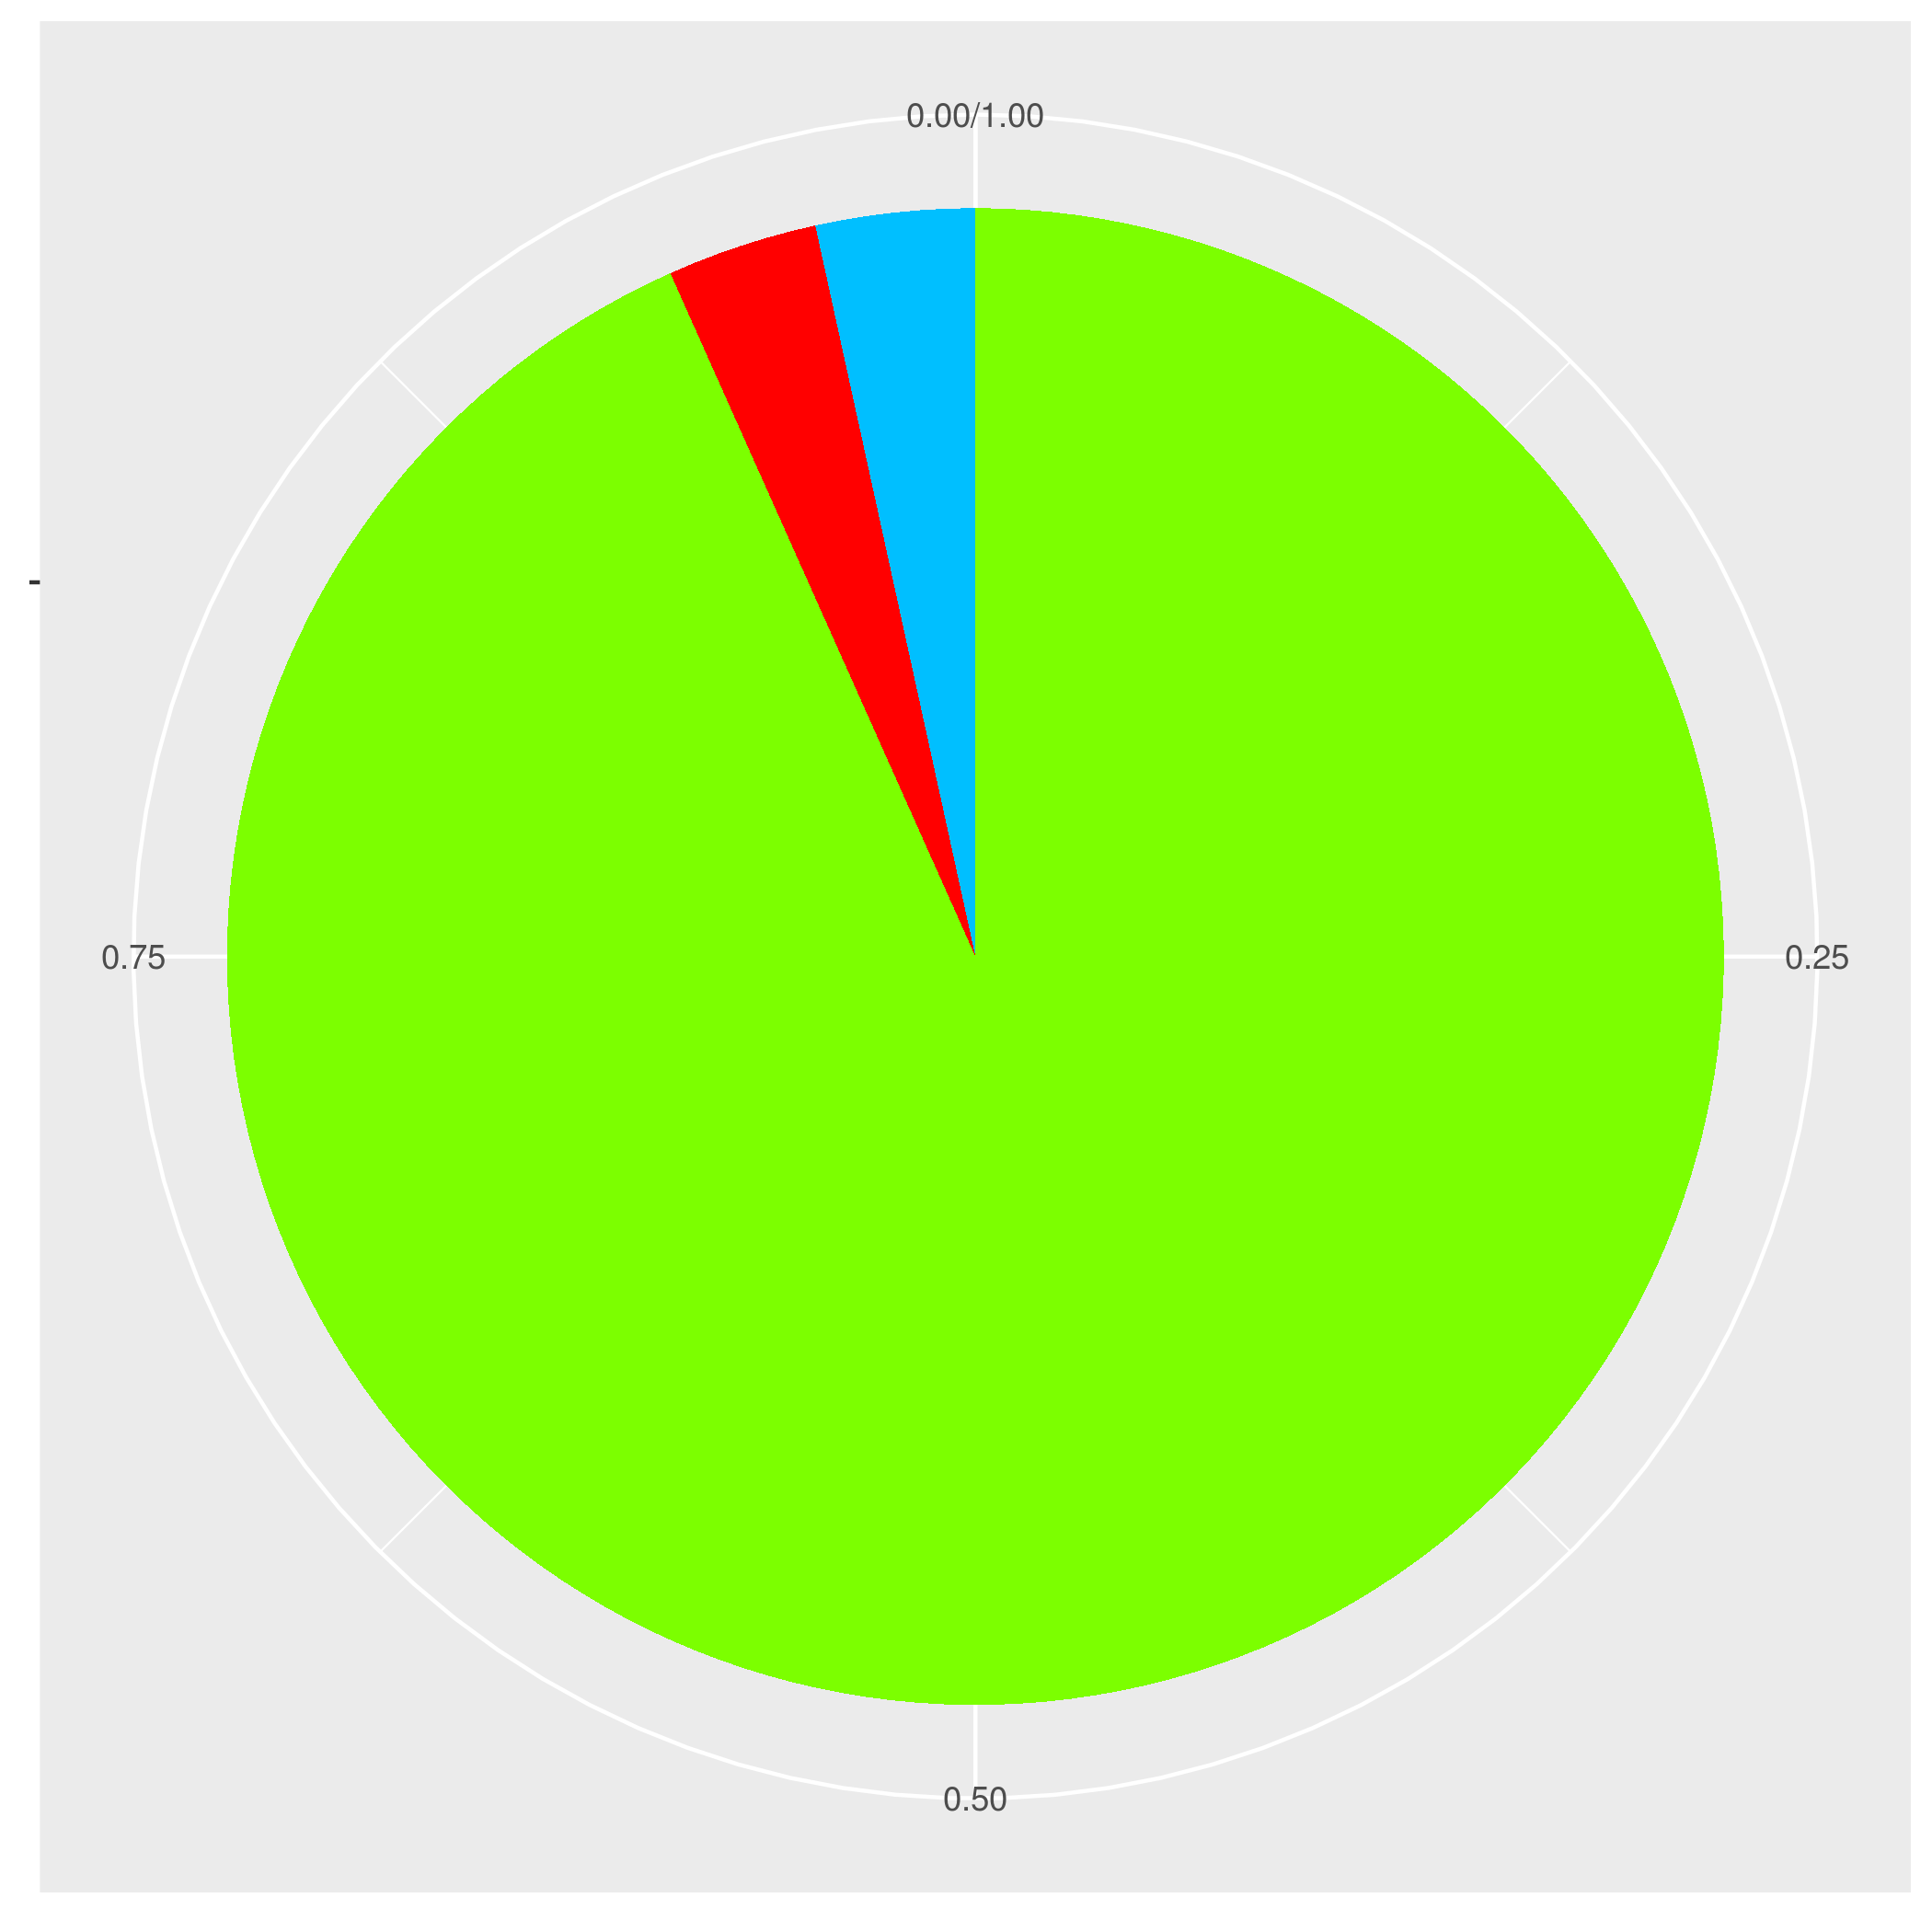
\includegraphics[width=.25\columnwidth]{kosarak.dat/riondato-c5.png}
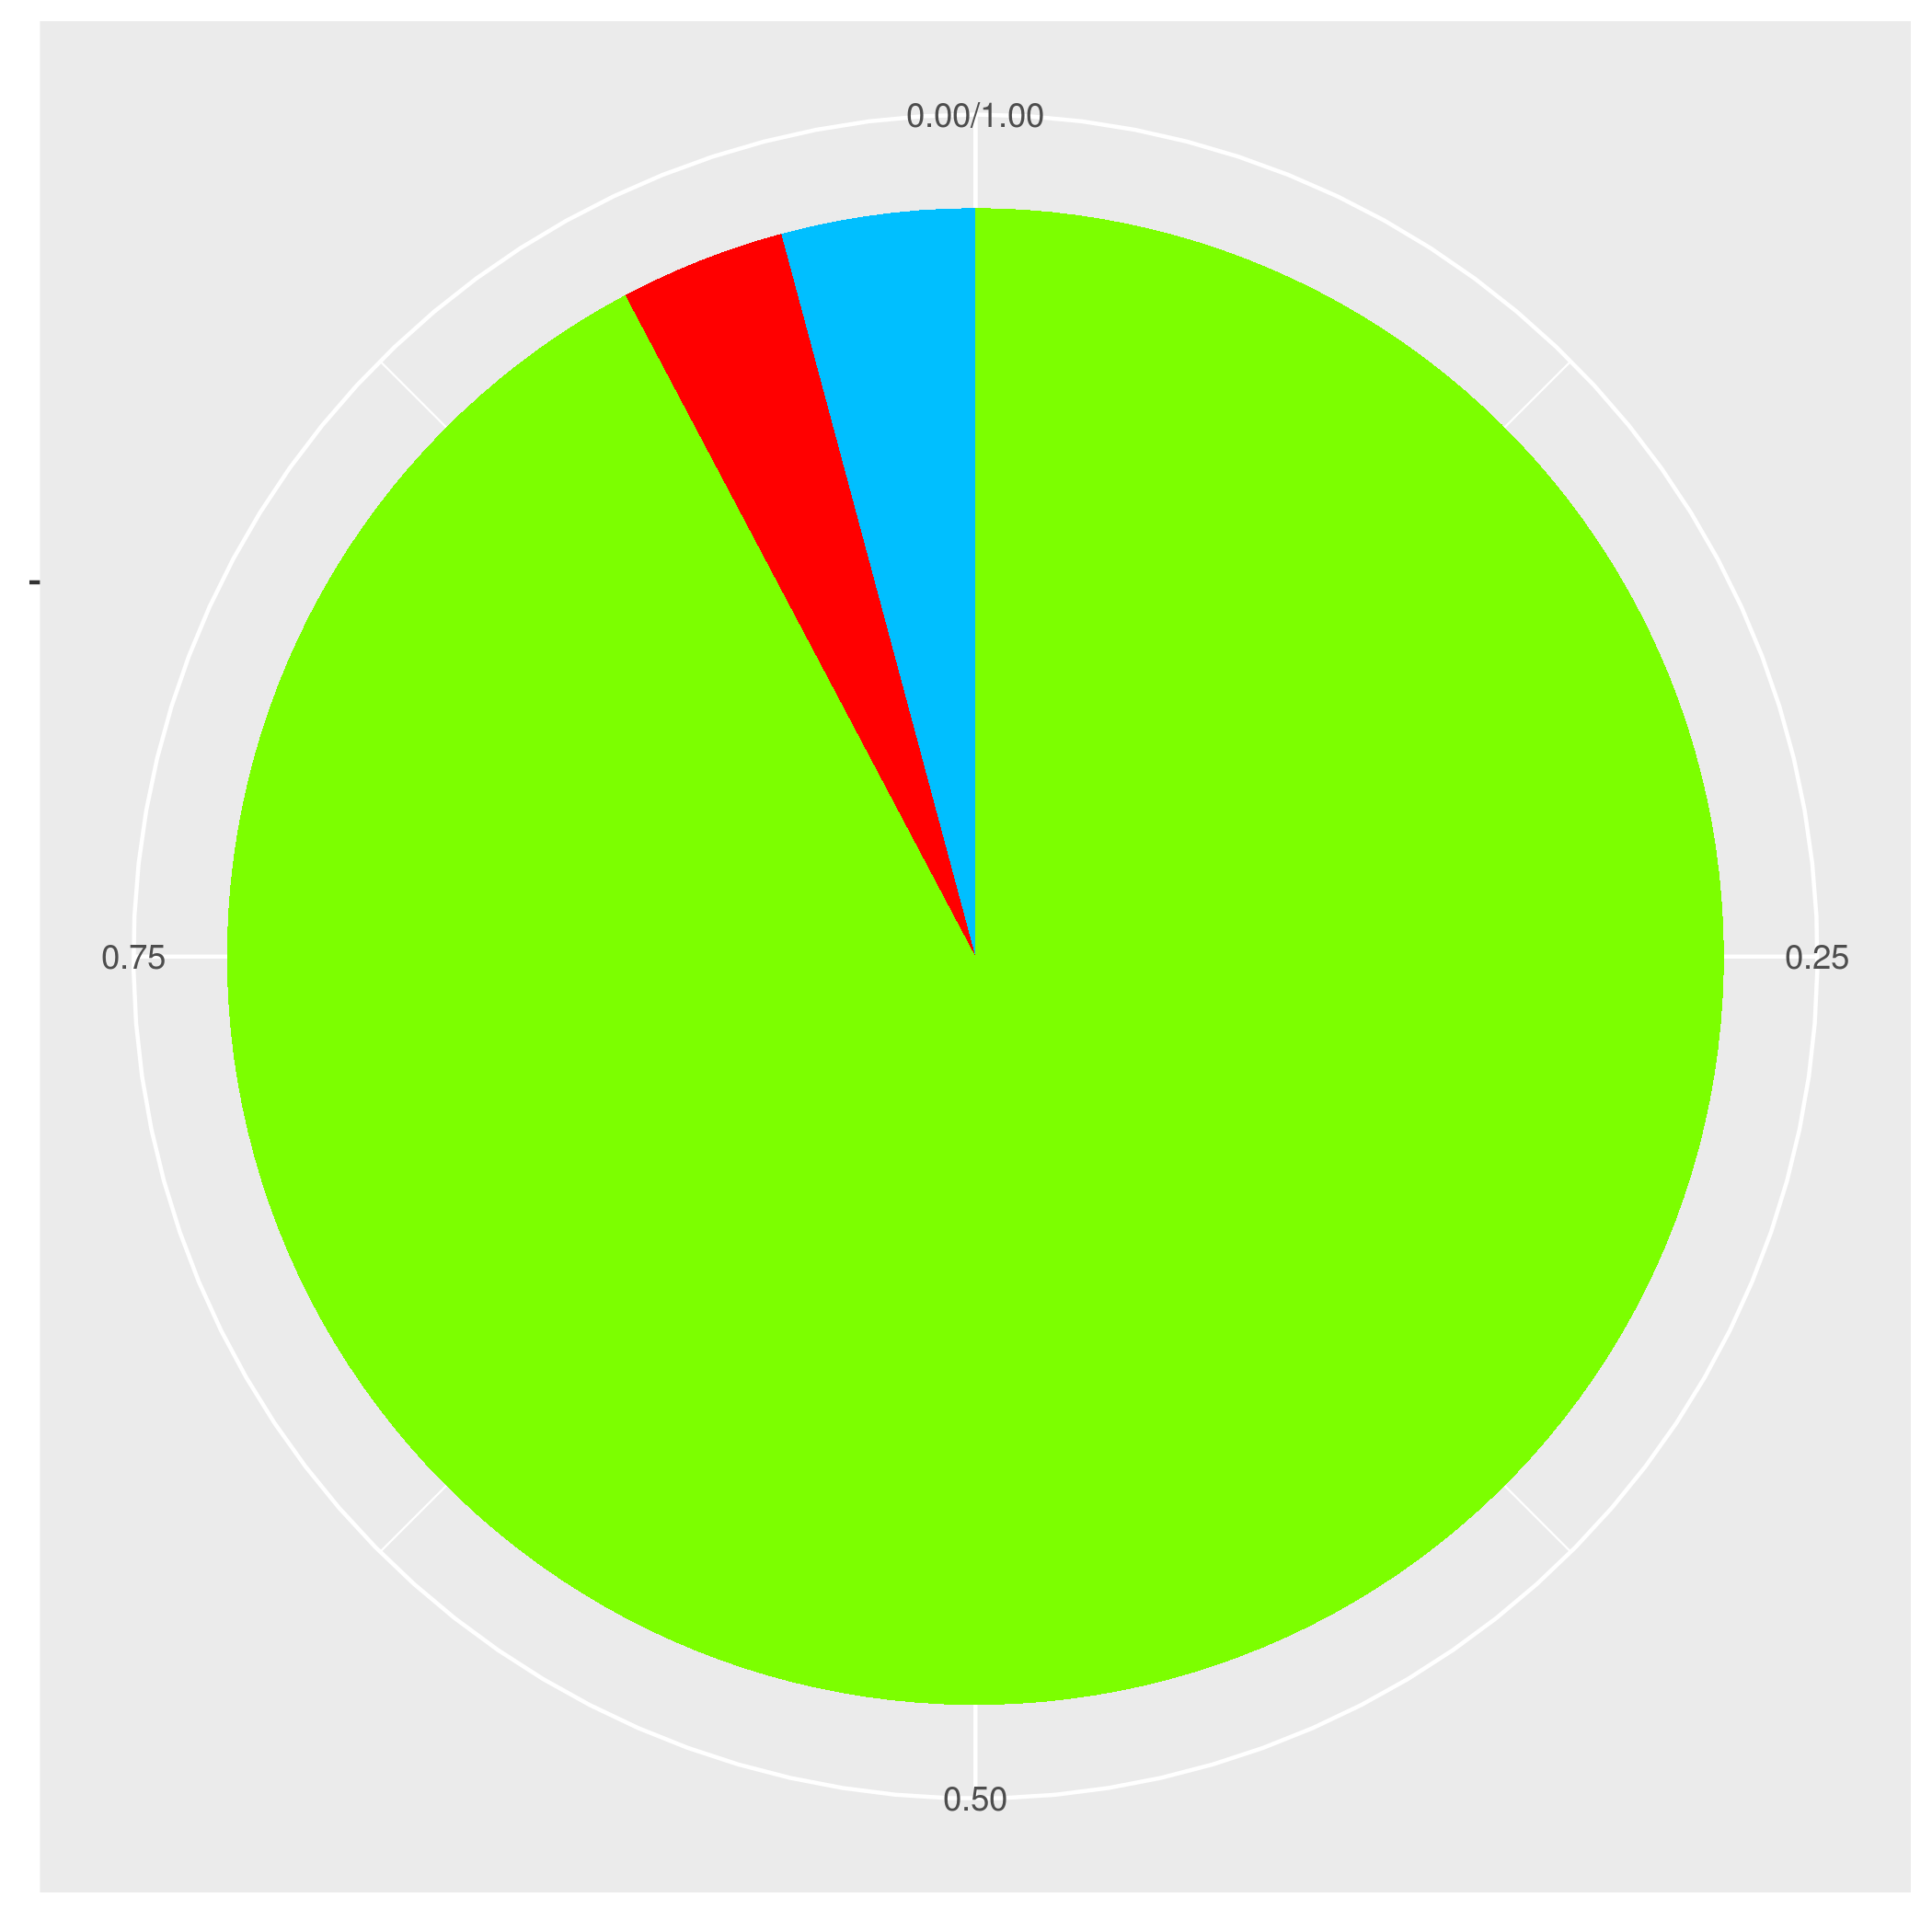
\includegraphics[width=.25\columnwidth]{kosarak.dat/riondato-c6.png}
\end{figure}

Concerning Riondato's technique, we can observe that looser settings classify too many non-frequent itemsets as frequent, while in stricter settings we get very reasonable and consistent behaviour.

More noteworthy is the fact that Toivonen's method is dominated by false-negatives, i.e. it misses almost all frequent itemsets. The reason is obvious; the samples are just too small for a dataset of this size and complexity.

\begin{center}
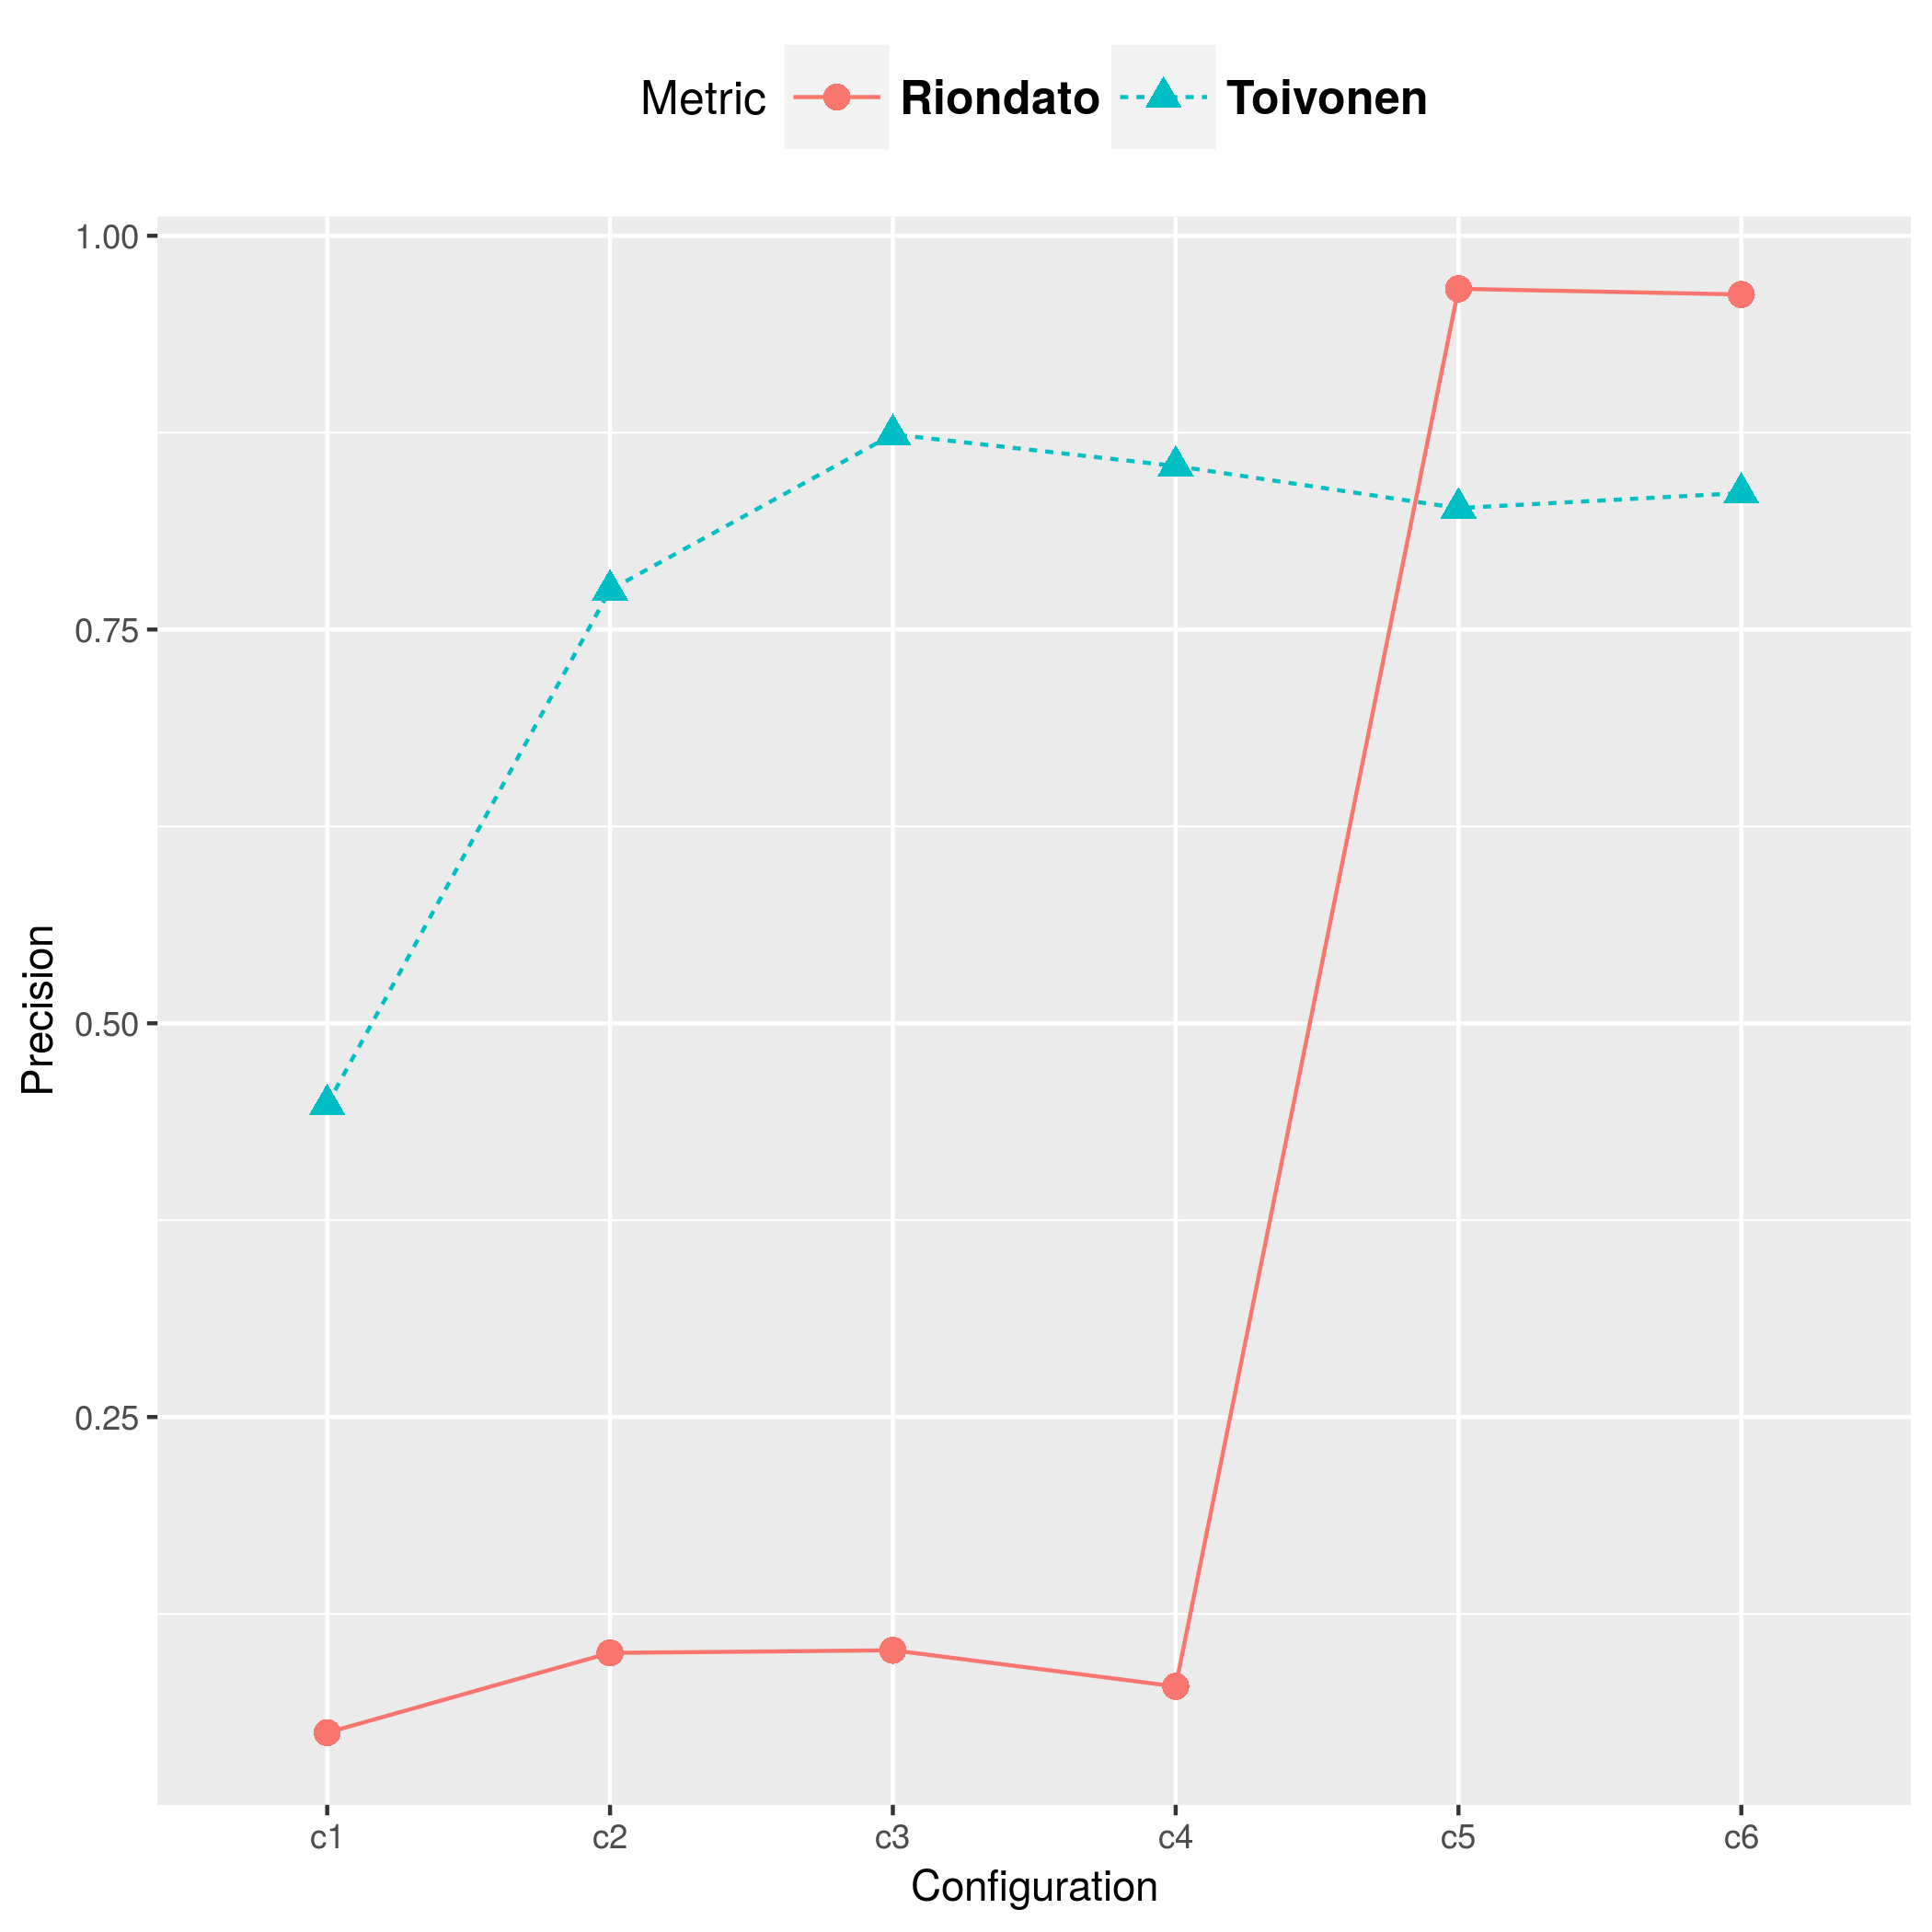
\includegraphics[width=.45\columnwidth]{kosarak.dat/precision.png}
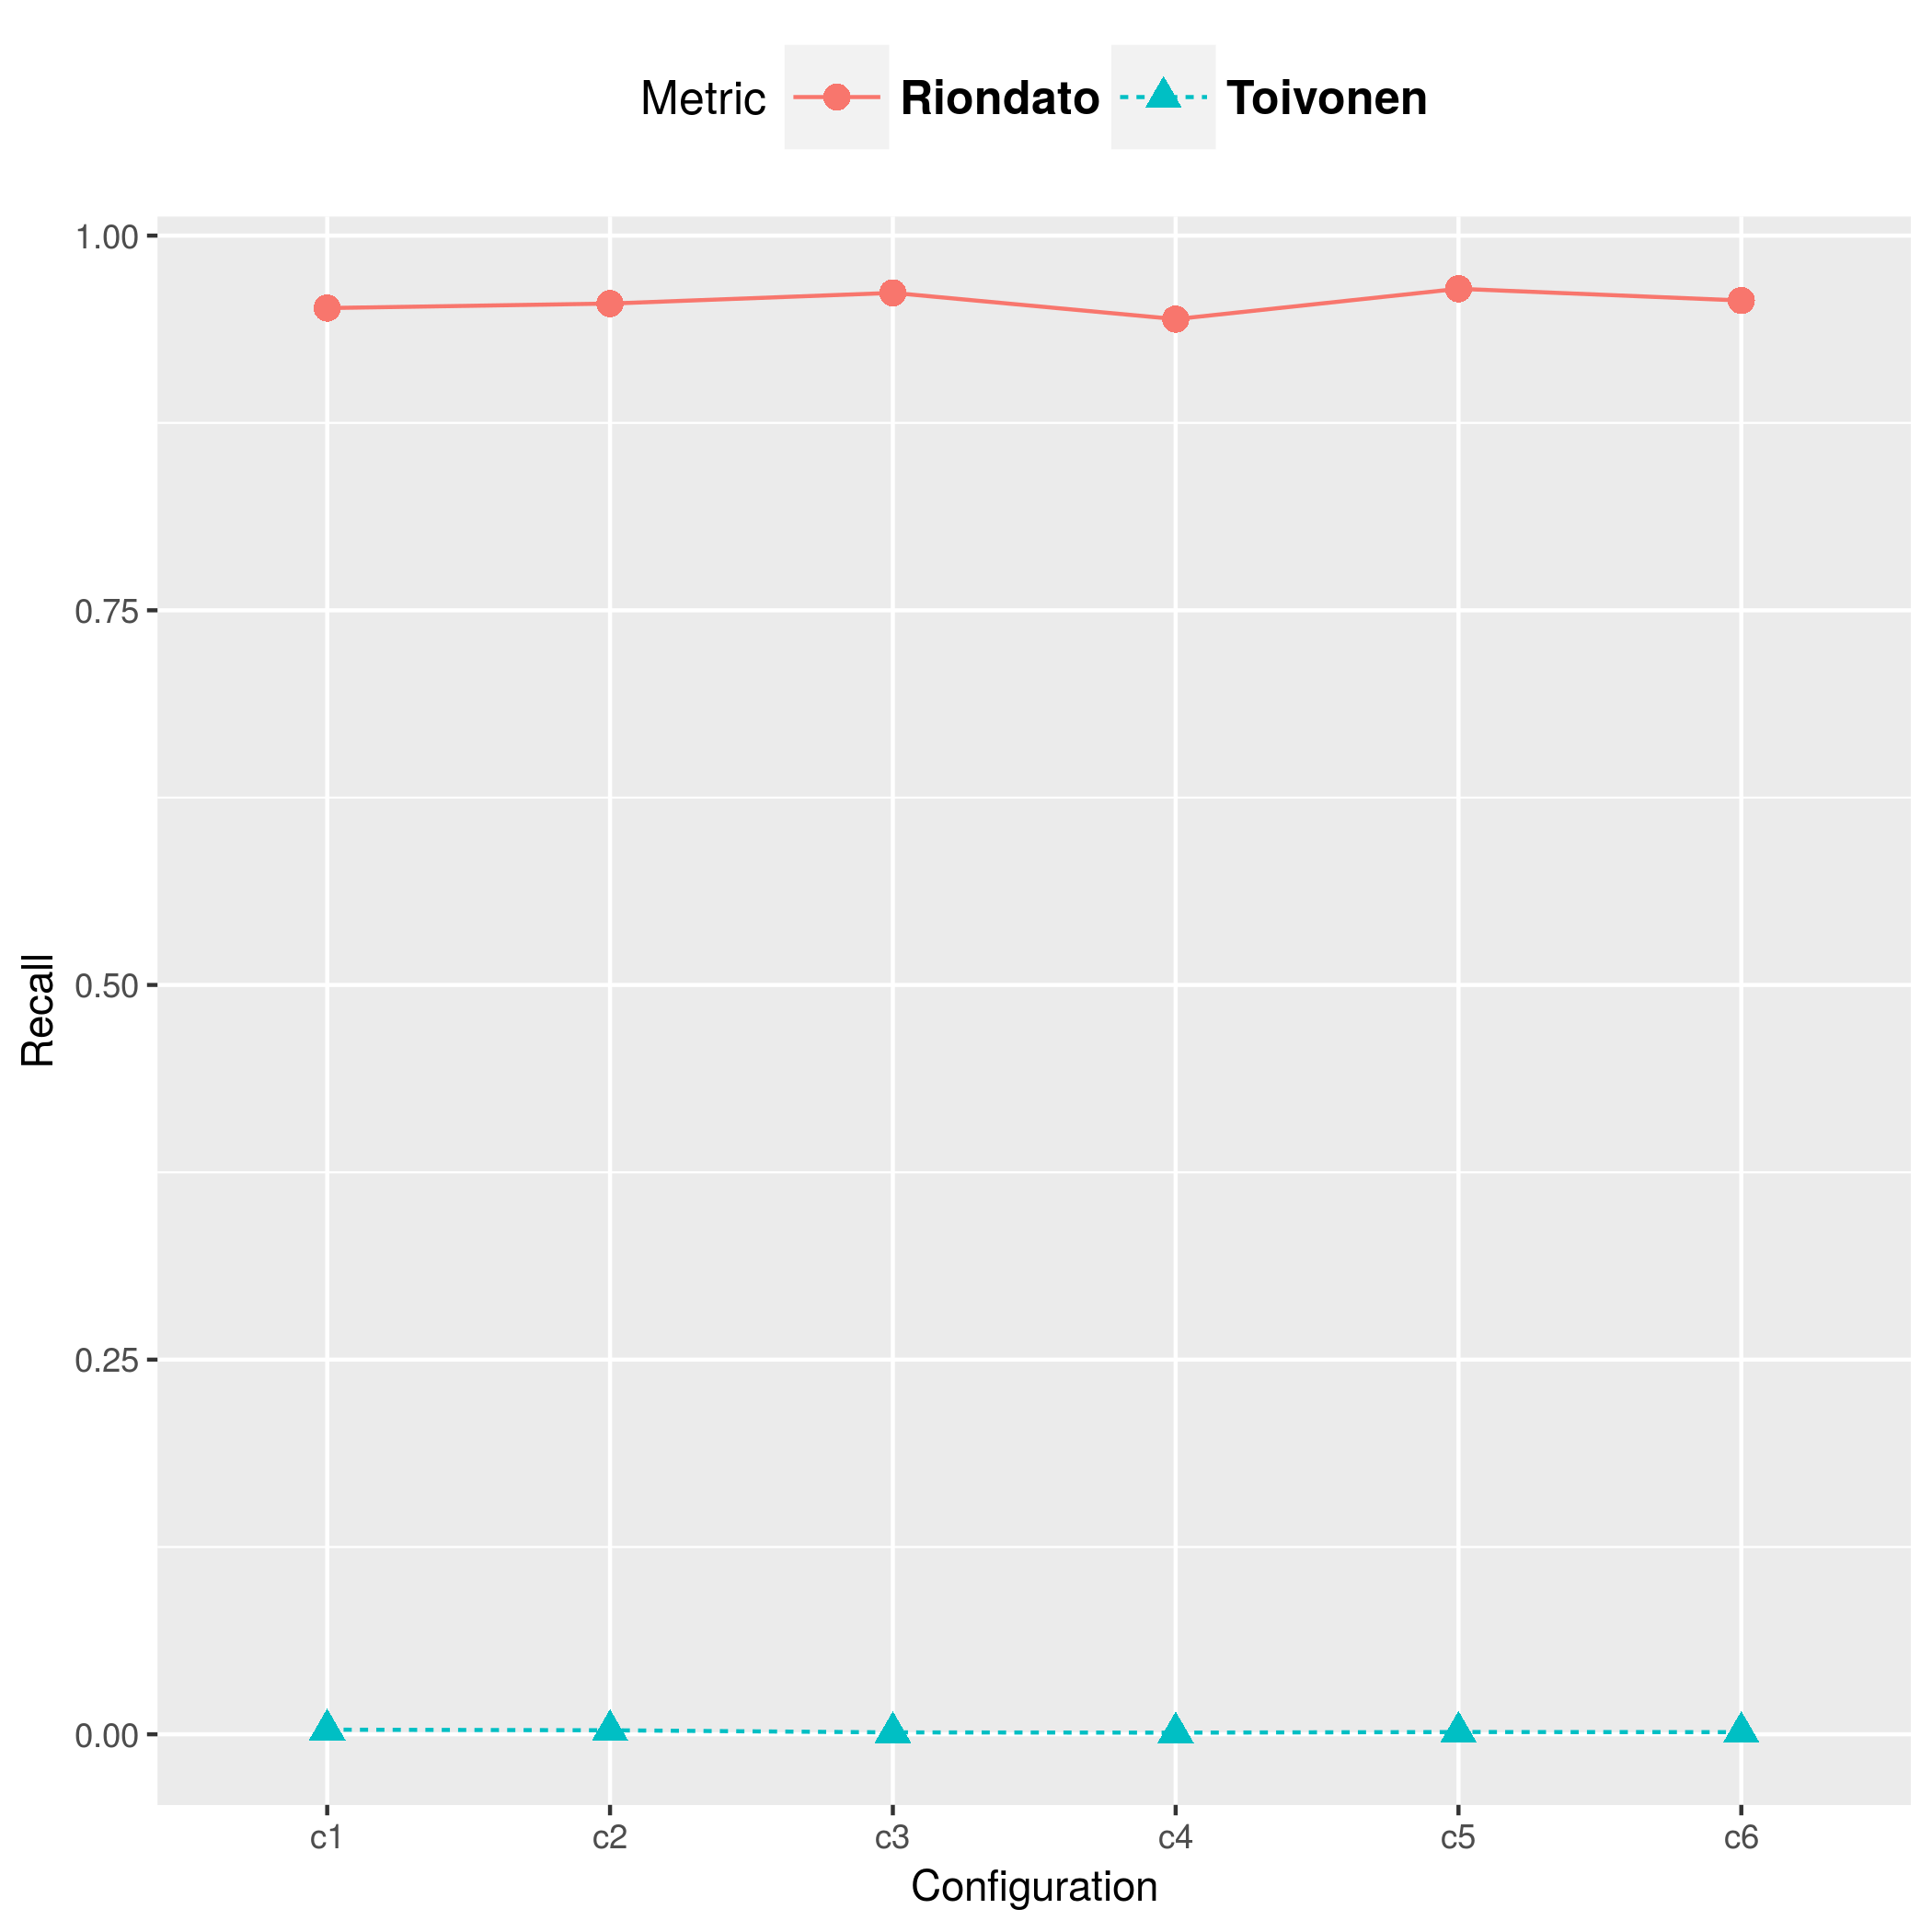
\includegraphics[width=.45\columnwidth]{kosarak.dat/recall.png}
\end{center}

\subsubsection{Frequency error}
\begin{figure}[h!]
\centering
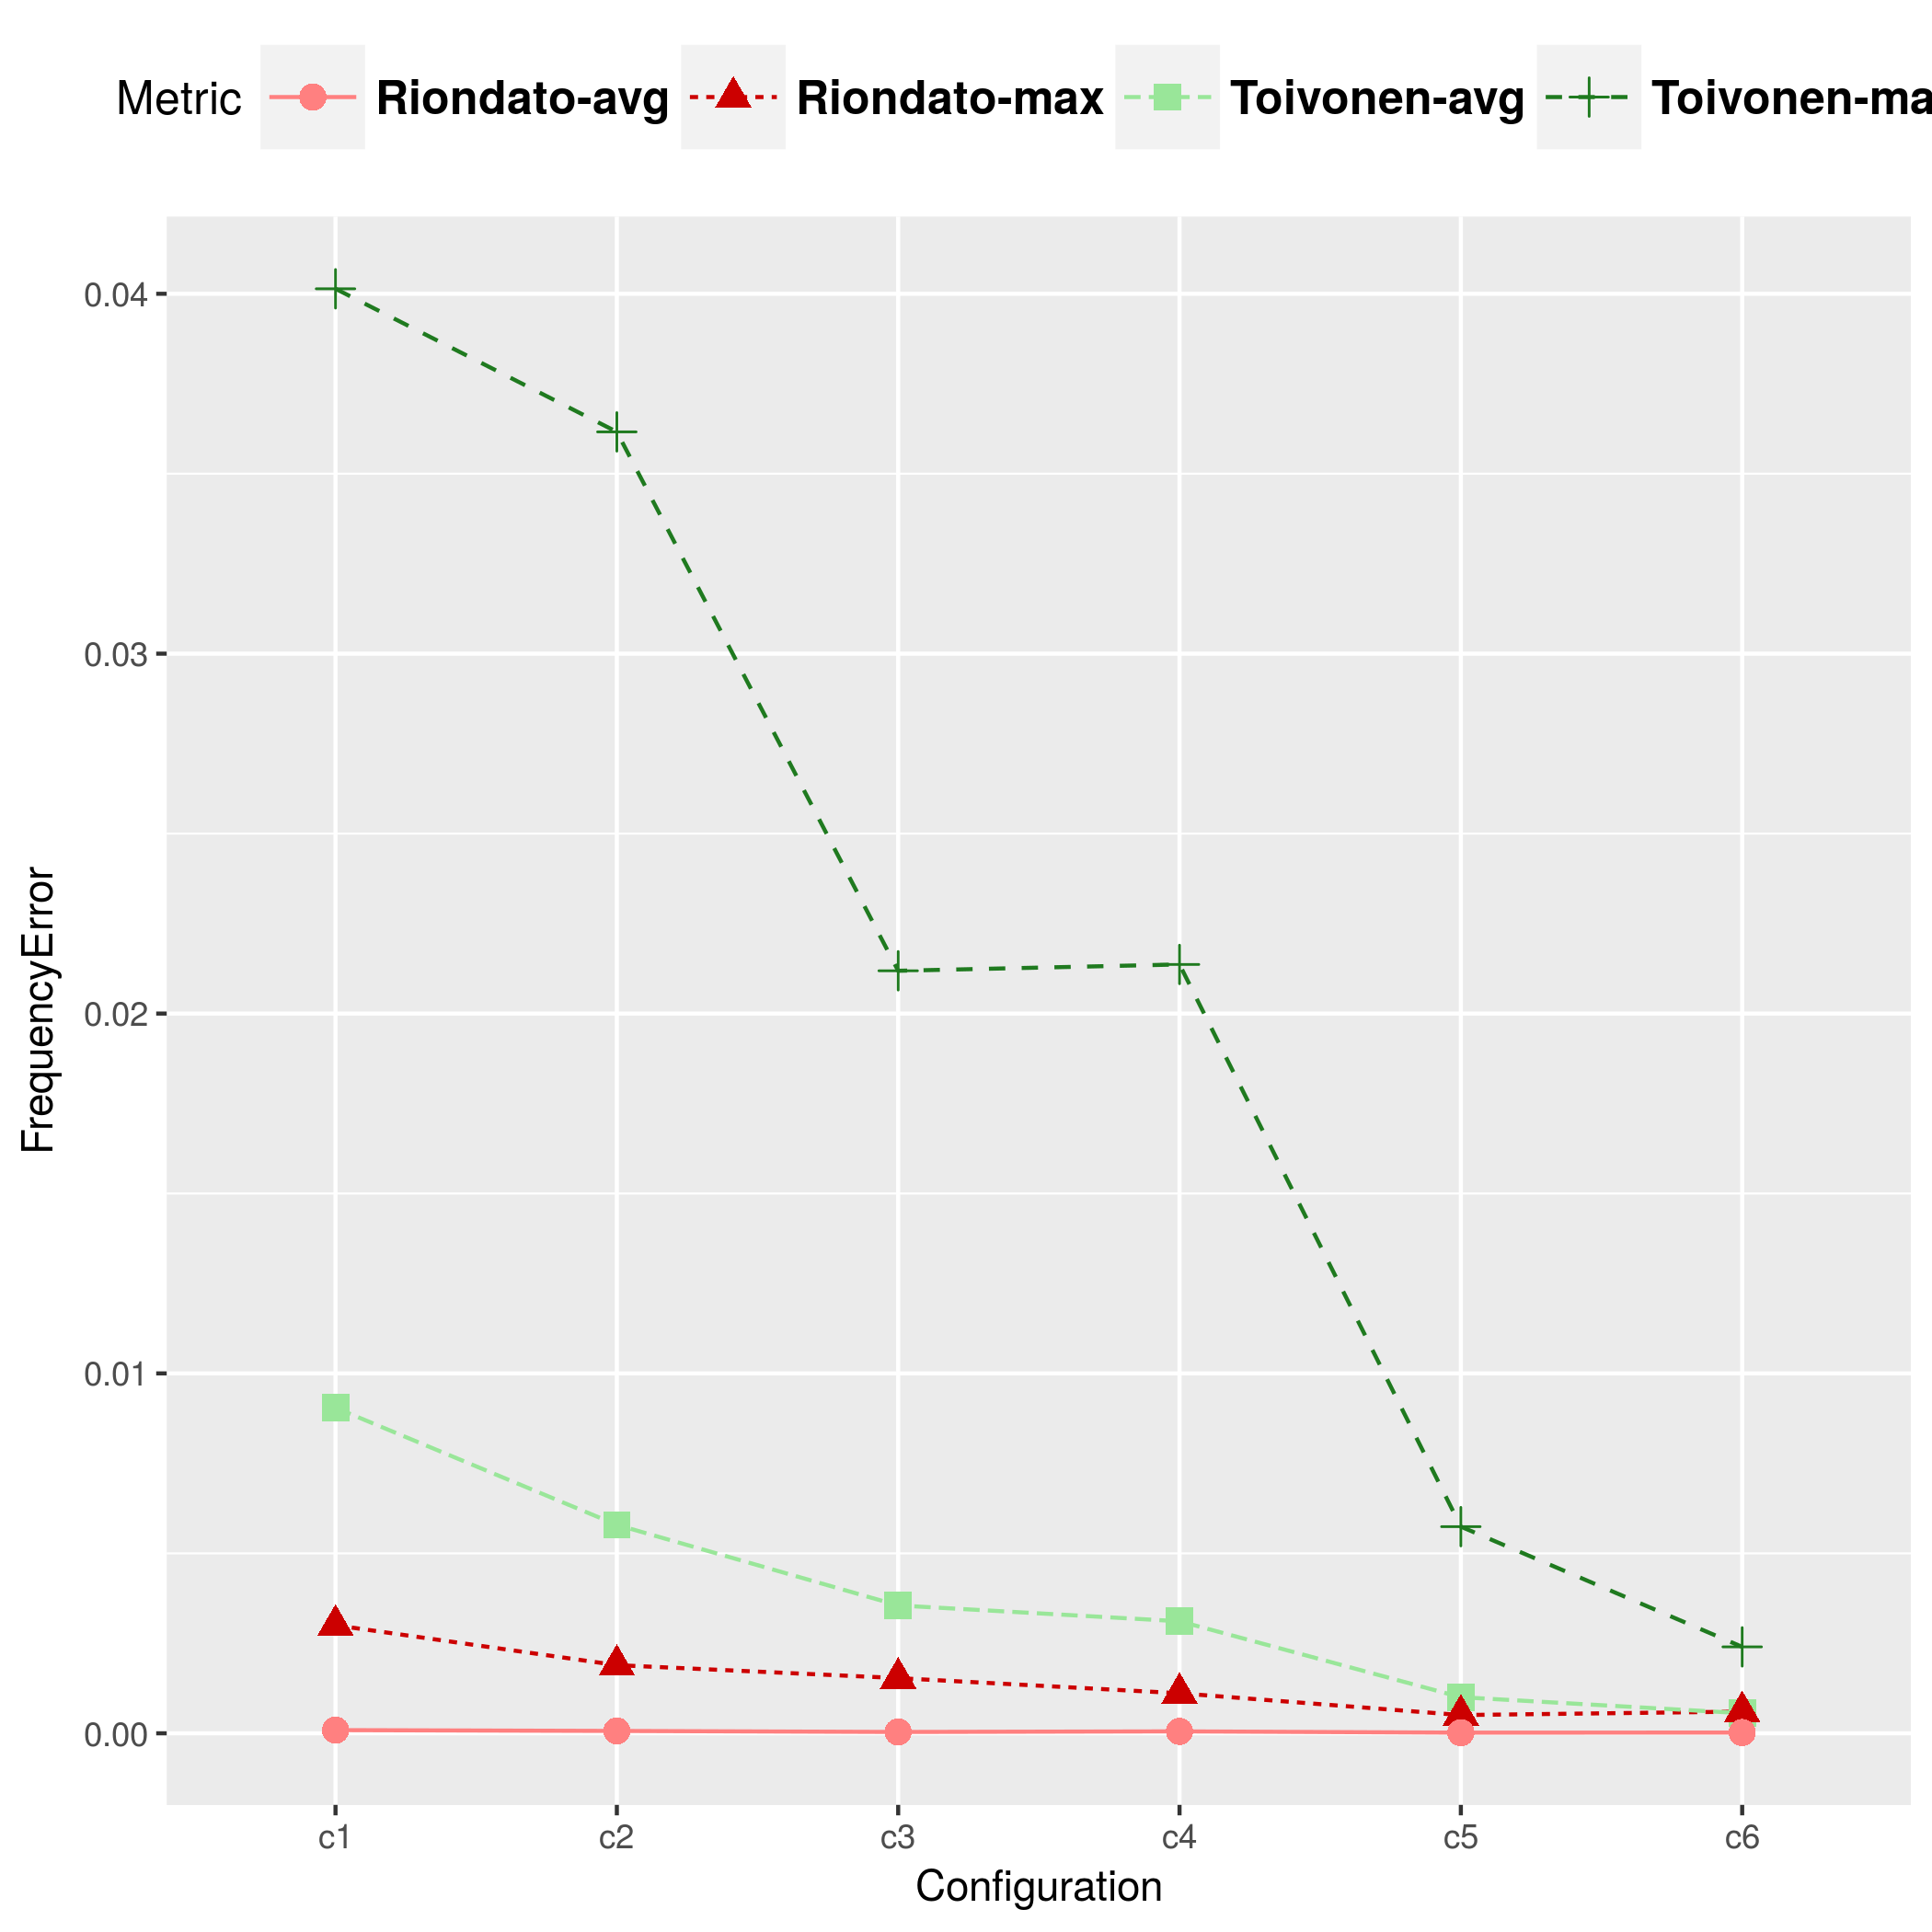
\includegraphics[width=.7\columnwidth]{kosarak.dat/freq.png}
\end{figure}
On the frequency estimation error, we can make roughly the same observations as before. Both approaches become more accurate, as we move to stricter parameters. Again, Riondato gives smaller errors and Toivonen suffer great maximum errors in loose settings.

\section{Conclusion}
To conclude, our measurements contradict Riondato's claim for smaller bounds of sample size. It is not the fact that the sample is linearly dependent on the number of items. This, in fact, is the reason behind Toivonen's low-quality results; it does not scale well with ever-larger dataset sizes.

Moreover, both methods seem to satisfy the user-defined thresholds in practice, since we got increasingly better results with stricter thresholds in all cases. More specifically, errors on support estimation get increasingly lower.

A major drawback of Toivonen's method is its extremely low precision, which can be attributed to the lowered minimum support threshold in which we mine against. Lowering this threshold is both a blessing and a curse, since we minimize the number of false-negatives (i.e. by lowering the possibility we miss a frequent itemset), but at the same time we dramatically increase the amount of false-positives (i.e. itemsets of support less than the minimum will actually be retrieved).

Last but not least, all experiments were developed in the R programming language, as well as the data plotting of the results. You can view the corresponding scripts in a Github repository\site{https://www.github.com/omelkonian/fim-experiment}, where we also host the same plots for all other datasets mentioned in Table \ref{tab:datasets}.

\end{document}
